% ============================================================
%  Jev and Beyond: A Survey of Calibration-Aware Decision-Making with Language Models
%  acmart acmsmall, nonacm (pdfLaTeX, \pdfoutput=1).
%  Build: python3 build/build_paper.py  (numbers, stage colours, pdflatex -> bibtex -> pdflatex x2).
%  Every number in sections/*.tex is a macro from sections/numbers.tex (build/gen_numbers.py).
% ============================================================
\pdfoutput=1
\PassOptionsToPackage{table}{xcolor}
\documentclass[acmsmall,screen,nonacm]{acmart}
\settopmatter{printacmref=false,authorsperrow=3}
\setcopyright{none}
\renewcommand\footnotetextcopyrightpermission[1]{}
\citestyle{acmauthoryear}

\usepackage{booktabs,array,pifont,longtable,adjustbox,xspace}
\usepackage[most]{tcolorbox}   % the block-mosaic taxonomy (Fig. 2)
\usepackage{tikz}
\usetikzlibrary{arrows.meta,shapes.geometric,positioning,fit,calc,patterns,decorations.pathreplacing}
\usepackage[edges]{forest}
% ============================================================
%  Shared taxonomy style: forked-edge forest (grow=east, reversed),
%  rounded
%  rectangles, per-category colour blocks.  Content colours are our
%  six robot-learning domains.
% ============================================================

% ---- draw + root ----
\definecolor{hidden-draw}{RGB}{40,40,40}
\definecolor{tx-root}{HTML}{D1D5DB}

% ---- per-domain category (darker) / leaf (lighter) fills ----
\definecolor{cat-code}{HTML}{93C5FD}\definecolor{leaf-code}{HTML}{DBEAFE}   % §3.1 blue
\definecolor{cat-vla}{HTML}{5EEAD4}\definecolor{leaf-vla}{HTML}{CCFBF1}     % §3.2 teal
\definecolor{cat-rew}{HTML}{FDBA74}\definecolor{leaf-rew}{HTML}{FEEBC8}     % §3.3 orange
\definecolor{cat-skill}{HTML}{C4B5FD}\definecolor{leaf-skill}{HTML}{EDE9FE} % §3.4 purple
\definecolor{cat-trans}{HTML}{F9A8D4}\definecolor{leaf-trans}{HTML}{FCE7F3} % §3.5 pink
\definecolor{cat-bench}{HTML}{86EFAC}\definecolor{leaf-bench}{HTML}{DCFCE7} % §3.6 green

% ---- per-sub-section palette (deep-dive figures: one colour per sub-section) ----
\definecolor{secA}{HTML}{93C5FD}\definecolor{secAl}{HTML}{DBEAFE} % blue
\definecolor{secB}{HTML}{5EEAD4}\definecolor{secBl}{HTML}{CCFBF1} % teal
\definecolor{secC}{HTML}{86EFAC}\definecolor{secCl}{HTML}{DCFCE7} % green
\definecolor{secD}{HTML}{FCD34D}\definecolor{secDl}{HTML}{FEF3C7} % amber
\definecolor{secE}{HTML}{FCA5A5}\definecolor{secEl}{HTML}{FEE2E2} % red (the gap)
\definecolor{secF}{HTML}{C4B5FD}\definecolor{secFl}{HTML}{EDE9FE} % purple
\definecolor{secG}{HTML}{F9A8D4}\definecolor{secGl}{HTML}{FCE7F3} % pink

% ---- the forest style, applied to every tree via default preamble ----
\forestset{
  default preamble={
    forked edges,
    for tree={
      grow=east,
      reversed=true,
      anchor=base west,
      parent anchor=east,
      child anchor=west,
      base=center,
      font=\large,
      rectangle,
      draw=hidden-draw,
      rounded corners,
      align=center,
      text centered,
      minimum width=5em,
      edge+={darkgray, line width=1pt},
      s sep=3pt,
      inner xsep=2pt,
      inner ysep=3pt,
      line width=0.8pt,
      ver/.style={rotate=90, child anchor=north, parent anchor=south, anchor=center},
      % per-level widths applied per node (reliable inside for tree)
      if level=1{text width=19em, font=\normalsize}{},
      if level=2{text width=33em, font=\normalsize}{},
    },
  },
}

\usepackage{pgfplots}\pgfplotsset{compat=1.18}
\newcommand{\yy}{\textcolor{green!55!black}{\ding{51}}}
\newcommand{\nn}{\textcolor{red!70!black}{\ding{55}}}
\newcommand{\pp}{\textcolor{orange!85!black}{$\sim$}}
\newcommand{\ab}{\textcolor{black!30}{--}}
\newcommand{\qq}{\textcolor{black!45}{?}}
% AUTO-GENERATED by build/build_paper.py from build/p05_common.py
\definecolor{stS0}{HTML}{8C8C8C}\colorlet{stS0txt}{stS0!70!black}\definecolor{stS1}{HTML}{4C78A8}\colorlet{stS1txt}{stS1!70!black}\definecolor{stS2}{HTML}{F58518}\colorlet{stS2txt}{stS2!70!black}\definecolor{stS3}{HTML}{54A24B}\colorlet{stS3txt}{stS3!70!black}\definecolor{stS4}{HTML}{B279A2}\colorlet{stS4txt}{stS4!70!black}\definecolor{stTH}{HTML}{8C6D1F}\colorlet{stTHtxt}{stTH!70!black}\definecolor{stX}{HTML}{E45756}\colorlet{stXtxt}{stX!70!black}
   % generated by build/build_paper.py from build/p05_common.py
% AUTO-GENERATED by build/gen_numbers.py -- do not hand-edit. Every number the prose uses.
\newcommand{\nWorks}{408\xspace}
\newcommand{\nSzero}{25\xspace}
\newcommand{\nSone}{52\xspace}
\newcommand{\nStwo}{54\xspace}
\newcommand{\nSthree}{121\xspace}
\newcommand{\nSfour}{80\xspace}
\newcommand{\nTheory}{5\xspace}
\newcommand{\nX}{71\xspace}
\newcommand{\nCore}{80\xspace}
\newcommand{\nLandscape}{323\xspace}
\newcommand{\nTOne}{23\xspace}
\newcommand{\nTTwo}{5\xspace}
\newcommand{\nTThree}{31\xspace}
\newcommand{\nTFour}{17\xspace}
\newcommand{\nTFive}{4\xspace}
\newcommand{\nCoreRL}{35\xspace}
\newcommand{\nTThreeRecent}{27\xspace}
\newcommand{\nTThreeTwentySix}{17\xspace}
\newcommand{\nCoreScore}{49\xspace}
\newcommand{\nCoreFree}{23\xspace}
\newcommand{\nCoreTyped}{7\xspace}
\newcommand{\nTyped}{65\xspace}
\newcommand{\nGuar}{66\xspace}
\newcommand{\nGuarSthree}{63\xspace}
\newcommand{\nCoreGuar}{1\xspace}
\newcommand{\nCoreAbstain}{21\xspace}
\newcommand{\nCoreNoAction}{45\xspace}
\newcommand{\nCoreECEonly}{11\xspace}
\newcommand{\nWhite}{221\xspace}
\newcommand{\nBlack}{126\xspace}
\newcommand{\nActAbstain}{39\xspace}
\newcommand{\nActHandOff}{35\xspace}
\newcommand{\nActRetrieve}{7\xspace}
\newcommand{\nActFilter}{20\xspace}
\newcommand{\nActAdapt}{18\xspace}
\newcommand{\nActSet}{30\xspace}
\newcommand{\nActNoAction}{259\xspace}
\newcommand{\nRefs}{451\xspace}
\newcommand{\nTaxShown}{77\xspace}
\newcommand{\nCoreRecent}{75\xspace}
\newcommand{\nCoreRecentPct}{94\%\xspace}
\newcommand{\nBgRecent}{166\xspace}
\newcommand{\nSzeroToSthree}{252\xspace}
\newcommand{\nBgRecentPct}{66\%\xspace}
\newcommand{\nContract}{93\xspace}
\newcommand{\nContractTyped}{65\xspace}
\newcommand{\nConstrained}{28\xspace}
\newcommand{\nTypedCal}{41\xspace}
\newcommand{\nCoreTypedCal}{7\xspace}
\newcommand{\nTypedReadPost}{40\xspace}
\newcommand{\nTypedReadPostCal}{24\xspace}
\newcommand{\nTypedTheory}{0\xspace}
\newcommand{\nTypedSthree}{11\xspace}
\newcommand{\nTypedX}{7\xspace}
\newcommand{\nTypedStwo}{0\xspace}
\newcommand{\nConstrainedAll}{32\xspace}
\newcommand{\nContractUnknown}{1\xspace}
\newcommand{\nTOneScore}{15\xspace}
\newcommand{\nTOneFree}{2\xspace}
\newcommand{\nTOneTyped}{6\xspace}
\newcommand{\nTOneOther}{0\xspace}
\newcommand{\nTTwoScore}{4\xspace}
\newcommand{\nTTwoFree}{0\xspace}
\newcommand{\nTTwoTyped}{0\xspace}
\newcommand{\nTTwoOther}{1\xspace}
\newcommand{\nTThreeScore}{27\xspace}
\newcommand{\nTThreeFree}{3\xspace}
\newcommand{\nTThreeTyped}{1\xspace}
\newcommand{\nTThreeOther}{0\xspace}
\newcommand{\nTFourScore}{2\xspace}
\newcommand{\nTFourFree}{15\xspace}
\newcommand{\nTFourTyped}{0\xspace}
\newcommand{\nTFourOther}{0\xspace}
\newcommand{\nTFiveScore}{1\xspace}
\newcommand{\nTFiveFree}{3\xspace}
\newcommand{\nTFiveTyped}{0\xspace}
\newcommand{\nTFiveOther}{0\xspace}
\newcommand{\nCoreOther}{1\xspace}
\newcommand{\nTFourAll}{17\xspace}
\newcommand{\nSurveysCompared}{39\xspace}
\newcommand{\nSurveysRecent}{33\xspace}
\newcommand{\nSurveys}{49\xspace}
\newcommand{\nSurveysPhaseOne}{32\xspace}
\newcommand{\nSurveysOffAxis}{10\xspace}
\newcommand{\nDup}{22\xspace}
\newcommand{\nMapped}{11\xspace}
\newcommand{\nCoreFourteen}{14\xspace}
\newcommand{\nRLRFull}{3\xspace}
\newcommand{\nStreams}{7\xspace}
\newcommand{\searchDate}{2026-09-26\xspace}
\newcommand{\nHF}{268\xspace}
\newcommand{\nHFNameOnly}{76\xspace}
\newcommand{\nHFUnverified}{4\xspace}
\newcommand{\nHFClassified}{188\xspace}
\newcommand{\nHFTrained}{137\xspace}
\newcommand{\nHFGeneralPct}{87\%\xspace}
\newcommand{\diTopSkill}{57.91\xspace}
\newcommand{\diSecondSkill}{57.44\xspace}
\newcommand{\nDISystems}{68\xspace}
\newcommand{\nDIBench}{38\xspace}
\newcommand{\nDICalBench}{32\xspace}
\newcommand{\nDIOneIn}{6\xspace}
\newcommand{\diRelease}{release 0.2.1\xspace}
\newcommand{\diDate}{2026-09-27\xspace}
\newcommand{\nDILowerECE}{17\xspace}
\newcommand{\nDIOpen}{67\xspace}
\newcommand{\nDIOpenWeights}{51\xspace}
\newcommand{\nDIFoundByName}{4\xspace}
\newcommand{\typedOtherStages}{A further 11 sit at extra inference and 7 among the consumers; none sit at prompt elicitation or among the theory works.\xspace}
\newcommand{\contractUnknownPhrase}{The contract of 1 work could not be determined from the paper.\xspace}
\newcommand{\coreOtherPhrase}{1 has another or an undetermined contract\xspace}
\newcommand{\coreTypedCalPhrase}{all of which report\xspace}
      % generated by build/gen_numbers.py
% ---- float placement: roomier float fractions; floats stay within their section ----
\usepackage{placeins}
\renewcommand{\topfraction}{0.9}\renewcommand{\bottomfraction}{0.5}
\renewcommand{\textfraction}{0.07}\renewcommand{\floatpagefraction}{0.85}
\setcounter{topnumber}{3}\setcounter{totalnumber}{4}


\begin{document}

\title[Jev and Beyond: A Survey of Calibration-Aware Decision-Making]{Jev and Beyond: A Survey of Calibration-Aware Decision-Making with Language Models}

\author{Gaytri Jena}
\authornote{The authors contributed to this work independently of their roles and employment.}
\affiliation{\institution{UC Berkeley}\city{Berkeley}\state{CA}\country{USA}}
\author{Kapil Wanaskar}
\authornotemark[1]
\affiliation{\institution{San Jose State University}\country{USA}}
\renewcommand{\shortauthors}{Jena and Wanaskar}

\begin{abstract}
A language model that is to act, and not only to converse, must state how likely each of its answers is
to be right, and software must be able to act on that number: answer, abstain, or hand the case off.
Calibration research long treated this confidence as something estimated after the fact, from token
probabilities, a post-hoc map, a prompted self-report or repeated sampling. Mostly since 2024, a second line
of work puts calibration into training itself, as a supervised objective or as a reward. This survey maps
both, with the training stage as its core. We collect \nWorks primary works and place each by
the stage at which calibration enters the decision pipeline: the model's own read-off, a post-hoc map,
prompt elicitation, extra inference, or training, plus the works that act on a confidence or fix the
output contract. The \nCore training-stage works, \nCoreRecent of them from 2024 to 2026, are organised
by what the training signal scores, in five families: supervised calibration objectives, reward-model
calibration, calibration rewards on the stated confidence, abstention and refusal training, and
process- and meaning-level confidence rewards. Every work is also classified by the output contract its
confidence is attached to. A typed decision, a probability for each declared
option, is common at the read-off and post-hoc stages, but only \nCoreTyped of the \nCore training works train
one; nearly all the rest train a stated score or a free-text hedge or refusal. Of the
\nSurveysCompared closest prior surveys, none organises calibration training across domains by what the
training signal scores, and none crosses that typology with the output contract. We close with seven
measurable quantities, each tied to a public testbed, and report the first of them, the calibration of
the decision itself, for Jev, a hosted typed-decision model, and \nDIOpen open decision models on a public
leaderboard.
\end{abstract}


\begin{CCSXML}
<ccs2012>
   <concept>
       <concept_id>10010147.10010178.10010179</concept_id>
       <concept_desc>Computing methodologies~Natural language processing</concept_desc>
       <concept_significance>500</concept_significance>
   </concept>
   <concept>
       <concept_id>10010147.10010257.10010258.10010261</concept_id>
       <concept_desc>Computing methodologies~Reinforcement learning</concept_desc>
       <concept_significance>500</concept_significance>
   </concept>
   <concept>
       <concept_id>10002950.10003648</concept_id>
       <concept_desc>Mathematics of computing~Probability and statistics</concept_desc>
       <concept_significance>300</concept_significance>
   </concept>
</ccs2012>
\end{CCSXML}
\ccsdesc[500]{Computing methodologies~Natural language processing}
\ccsdesc[500]{Computing methodologies~Reinforcement learning}
\ccsdesc[300]{Mathematics of computing~Probability and statistics}

\keywords{calibration, uncertainty, language models, reinforcement learning, proper scoring rules,
  abstention, conformal prediction, structured output, decision-making, survey}

\maketitle

\section{Introduction}
\label{sec:intro}

A language model that automates a step in a program has to do more than produce a good answer. It has
to say how likely that answer is to be right, in a form that the program can act on: answer when the
probability is high, and abstain or hand the case to another model or a person when it is not. The rule
is only as good as the number it reads. A confidence is \emph{calibrated} when, among the cases to which
the model gives probability $p$, a fraction $p$ is correct~\citep{guo2017calibration}; a threshold
policy built on a miscalibrated confidence answers when it should not, or escalates cases it could have
settled.

% AUTO-GENERATED by build/gen_jev_market.py from literature/notes/jev_hf_268.tsv -- do not hand-edit.
\begin{table}[tp]
\centering\footnotesize
\renewcommand{\arraystretch}{1.18}
\caption{\textbf{Repositories returned by the Hugging Face model search for ``jev'', by application} (snapshot of
2026-09-27). \href{https://typesafe.ai/blog/introducing-system-one-models-and-jev}{Jev} is a hosted model from TypeSafe AI, released on 2026-09-15~\citep{almeida2026introducing},
that returns a probability for each declared option (a typed decision, Table~\ref{tab:definitions}). Of the 268
repositories the search returns, 76 only share the name (75 predate Jev) and 4
could not be verified (empty, without a card, or gated with no public card metadata); the remaining 188 are classified here from their
model cards and file lists (for a gated repository, from its public card metadata), with an application category taking
precedence over a language one. Downloads are over the last
30 days. 137 repositories contain newly trained weights; the 38 copies, ports and packages add
none (the 6 mirrors contain their source's weight files byte for byte). General-purpose models and the
copies of them account for 87\% of the 41,653 downloads in the table. A name search misses most decision models: of the
51 open systems with released weights on the Jev Decision Index (Table~\ref{tab:jev_decision_index}), it returns 4.}
\Description{A table with one row per application category of the repositories returned by the Hugging Face search for jev,
giving the number of repositories, their downloads over thirty days and linked example repositories. General-purpose typed-decision models are
the largest group, followed by research checkpoints and copies.}
\label{tab:jev_hf_ecosystem}
\begin{tabular}{@{}>{\raggedright\arraybackslash}p{0.24\textwidth}rr>{\raggedright\arraybackslash}p{0.45\textwidth}@{}}
\toprule
\textbf{Category} & \textbf{Repositories} & \textbf{Downloads} & \textbf{Examples} \\
\midrule
General-purpose typed-decision model & 55 & 19,655 & \href{https://huggingface.co/alibiserikbay/JevK5}{JevK5}, \href{https://huggingface.co/ZefanCai/Open-Jev-9B}{Open-Jev-9B}, \href{https://huggingface.co/com-kotobalabs/open-jev-deberta-v3-large}{open-jev-deberta}, \href{https://huggingface.co/lostargon/Tiny-Jev}{Tiny-Jev}, \href{https://huggingface.co/chaoliangUNSW/Jev-Style-0.8B-Decision-v3}{Jev-Style v3} \\
Research and ablation checkpoints & 45 & 212 & \href{https://huggingface.co/Praveenrajus/jevify-qwen3.5-4b-readout-coh}{jevify} (31-checkpoint readout series), \href{https://huggingface.co/JonesLin/next-jev-stage1-cot}{next-jev} (latent-workspace study), \href{https://huggingface.co/ryandcunha/mmbu-jev-qwen3-0.6b-closed}{mmbu-jev} (closed-set vs free-text) \\
Copy, port or package (no new training) & 38 & 18,640 & \href{https://huggingface.co/mradermacher/JEV-9B-GGUF}{JEV-9B-GGUF} (GGUF), \href{https://huggingface.co/Ruiruiz30/Jev-Omni-MLX-4bit}{Jev-Omni-MLX-4bit} (MLX), \href{https://huggingface.co/onnx-community/open-jev-deberta-v3-large-ONNX}{open-jev-deberta-ONNX} (ONNX), \href{https://huggingface.co/liodon-ai/JevK5-FP8}{JevK5-FP8} (FP8), \href{https://huggingface.co/junetask/Open-Jev-9B}{junetask/Open-Jev-9B} (a mirror) \\
No newly trained model (recipe, runtime, code or data) & 11 & 0 & \href{https://huggingface.co/NicolaiMTLassen/bonzi-8b-v1-jev}{bonzi} (recipes), \href{https://huggingface.co/Meanblock/JEV-CPU}{JEV-CPU} (code), \href{https://huggingface.co/SargeDev/jev-distill-corpus}{jev-distill-corpus} (dataset) \\
Agents, tools and safety & 10 & 1,005 & \href{https://huggingface.co/samatv256/mini-Jev}{mini-Jev} (tool routing), \href{https://huggingface.co/nicolasembleton/mini-jev-minicpm5-2b-shell-safety-phase1b-merged}{Mini-Jev shell-safety}, \href{https://huggingface.co/SargeDev/jev-gate-student-b}{Jev-Gate} (memory gating), \href{https://huggingface.co/atmaneayoub/jev-ar}{jev-ar} (Gulf-Arabic intent routing) \\
Domain application & 10 & 152 & \href{https://huggingface.co/Nebulaw1/jev-qwen3.5-4b-legal-lora}{jev-legal} (Chinese legal), \href{https://huggingface.co/mogita/jev-decider-qwen3-4b}{jev-decider} (bank transactions), \href{https://huggingface.co/guzus/jev-nyotti}{jev-nyotti} (BTC trading), \href{https://huggingface.co/wendellperbar/serigy-jev}{Serigy-Jev} (PT-BR fake news), \href{https://huggingface.co/sdmlai/nano-jev}{Nano-Jev} (RAG) \\
Language-specific & 7 & 1,010 & \href{https://huggingface.co/argos1111/modernbert-ja-310m-jev}{modernbert-ja-jev} (Japanese), \href{https://huggingface.co/wwydmanski/bielik-minitron-jev-v0.3}{bielik-minitron-jev} (Polish), \href{https://huggingface.co/nouton/jev-ru-4b-lora-v2}{Jev-RU} (Russian, Ukrainian, Belarusian) \\
Multimodal or vision & 5 & 594 & \href{https://huggingface.co/akhilaaa3/Jev-Omni}{Jev-Omni} (text, image, audio, video), \href{https://huggingface.co/SeanLiu/Jev-Vision}{Jev-Vision}, \href{https://huggingface.co/Fr0zencr4nE/jev-spatial}{Jev-Spatial} \\
Games and control & 5 & 156 & \href{https://huggingface.co/SUPER321/jevflash-doom-basic-0.6b}{JevFlash} (Doom), \href{https://huggingface.co/bzantium/gemma-3-270m-jev}{gemma-3-270m-jev} (ViZDoom), \href{https://huggingface.co/zwh20081/hoi4-jevai}{JevAI} (Hearts of Iron IV mod) \\
Embeddings trained on typed-decision questions & 2 & 229 & \href{https://huggingface.co/HIT-TMG/JevEmbed-KaLM-Embedding-V2.5}{JevEmbed-KaLM}, \href{https://huggingface.co/HIT-TMG/JevEmbed-Qwen3-Embedding-0.6B}{JevEmbed-Qwen3} \\
\midrule
\textbf{Total} & \textbf{188} & \textbf{41,653} & \\
\bottomrule
\end{tabular}
\end{table}

% AUTO-GENERATED by build/gen_jev_market.py from literature/notes/jev_decision_index_2026-09-27.json -- do not hand-edit.
\begin{table}[tp]
\centering\footnotesize
\setlength{\tabcolsep}{3.5pt}
\caption{\textbf{Jev and open decision models on the Jev Decision Index}: ranks 1 to 15 of the 68
systems on the \href{https://huggingface.co/spaces/multimodalart/jev-decision-index}{Jev Decision Index}~\citep{multimodalart2026jevdi} (release 0.2.1,
data of 2026-09-27). Skill is chance-normalised (0 to 100) over the same 38-benchmark
panel for every system, and unanswered requests count as wrong. ECE is measured on a one-in-6
sample of 32 benchmarks with a per-field right answer. The board reports point estimates
without uncertainty intervals. Base model and method are as recorded by the board: full fine-tune, a low-rank adapter (LoRA), a trained head or adapter over a frozen model, inference only (prompting or decoding over unchanged weights) or a hosted API. Names link to the
model's Hugging Face repository, or to its code where no weights are released. Jev ranks 1 on skill;
across the whole board, 17 of the 67 open systems have a lower ECE than Jev.}
\Description{A table of the fifteen highest-ranked decision models on the Jev Decision Index, with base model, adaptation method,
skill score and expected calibration error.}
\label{tab:jev_decision_index}
\begin{tabular}{@{}rlllrr@{}}
\toprule
\textbf{Rank} & \textbf{System} & \textbf{Base model} & \textbf{Method} & \textbf{Skill} & \textbf{ECE} \\
\midrule
1 & \href{https://typesafe.ai/blog/introducing-system-one-models-and-jev}{Jev 1.13 (TypeSafe AI, hosted)} & not disclosed & hosted API & 57.91 & 0.074 \\
2 & \href{https://huggingface.co/surogate/rune-26b-a4b-GGUF}{Surogate Rune 26B-A4B v3 [bf16]} & gemma-4-26B-A4B-it & full fine-tune & 57.44 & 0.120 \\
3 & \href{https://github.com/Mapika/decider}{Decider chat · Gemma-4-31B} & gemma-4-31B & inference only & 57.33 & 0.047 \\
4 & \href{https://huggingface.co/denis-pplx/autojev-27b}{AutoJev-27B} & Qwen3.8-27B & full fine-tune & 56.40 & 0.018 \\
5 & \href{https://github.com/featherless-ai/simple-jev}{simple-jev · Qwen3.8-27B (featherless)} & Qwen3.8-27B & inference only & 55.74 & 0.113 \\
6 & \href{https://huggingface.co/frontier-infra/jebadiah-27b}{Jebadiah 27B} & Qwen3.8-27B & LoRA & 54.67 & 0.014 \\
7 & \href{https://github.com/kshetrajna12/reflex}{reflex 27B [FP8 · wide choice]} & Qwen3.8-27B & inference only & 52.16 & 0.024 \\
8 & \href{https://github.com/Mapika/decider}{Decider chat · Qwen3.6-27B} & Qwen3.6-27B & inference only & 51.35 & 0.021 \\
9 & \href{https://huggingface.co/EldanRing/Winnow-12B}{Winnow-12B [Q8\_0]} & gemma-4-12B & LoRA & 50.02 & 0.168 \\
10 & \href{https://github.com/JoshuaSP/open-jev}{JoshuaSP diffusiongemma (open-jev)} & diffusiongemma-26B-A4B-it & inference only & 49.47 & 0.216 \\
11 & \href{https://github.com/kikoncuo/jevfire}{Jevfire} & Qwen3.8-27B & inference only & 49.37 & 0.052 \\
12 & \href{https://huggingface.co/Mapika/decider-35b-a3b-nvfp4}{Decider 35B-A3B [NVFP4]} & Qwen3.5-35B-A3B-Base & full fine-tune & 47.11 & 0.023 \\
13 & \href{https://huggingface.co/kirp/jpt-9b}{JPT-9B} & Qwen3.5-9B-Base & LoRA & 46.89 & 0.077 \\
14 & \href{https://huggingface.co/llm-semantic-router/Decision-1.0-Lux-9B}{Decision 1.0 Lux} & Qwen3.5-9B-Base & head or adapter & 43.49 & 0.076 \\
15 & \href{https://huggingface.co/juspay/xor}{Xor} & Qwen3.6-35B-A3B & full fine-tune & 41.48 & 0.015 \\
\bottomrule
\end{tabular}
\end{table}


\paragraph{Public typed-decision models.} Tables~\ref{tab:jev_hf_ecosystem} and~\ref{tab:jev_decision_index} record
two public views of the typed-decision models available on \diDate; every row links to the model, so a reader
can try one directly. Table~\ref{tab:jev_hf_ecosystem} classifies the \nHF repositories that the
Hugging Face model search for ``jev'' returns: \nHFNameOnly only share the name, \nHFUnverified could not be
verified, and \nHFClassified were classified from their model cards and file lists; \nHFTrained contain newly
trained weights, and general-purpose models with their copies account for \nHFGeneralPct of downloads. A name
search is a poor census of decision models: of the \nDIOpenWeights open systems with released weights on the
leaderboard of Table~\ref{tab:jev_decision_index}, it returns \nDIFoundByName. Table~\ref{tab:jev_decision_index}
lists the top of that leaderboard, the Jev Decision Index~\citep{multimodalart2026jevdi} (\diRelease), which
scores \nDISystems systems on skill over \nDIBench decision benchmarks and on the calibration of the chosen
option. Jev, a hosted model from TypeSafe AI released on 15 September 2026~\citep{almeida2026introducing},
returns a probability for each declared option; it is not one of the \nWorks works in our corpus, and its
base model is not disclosed. Neither view is peer reviewed, and neither is used to rank the training
families of Section~\ref{sec:core}.


For most of the literature, the confidence of a language model is estimated \emph{after} the model has been
trained. It is
read off the model's own token or sequence probabilities, which are well calibrated on multiple-choice
formats for large pretrained models~\citep{kadavath2022language} but lose calibration after
post-training~\citep{openai2023gpt4}; it is rescaled by a post-hoc map fitted on held-out
data~\citep{guo2017calibration}; it is requested in words or numbers through the
prompt~\citep{tian2023just}, where stated confidences cluster near the top of the
scale~\citep{xiong2023can}; or it is computed from extra inference, such as the agreement of sampled
answers or a conformal prediction set~\citep{farquhar2024semantic,campos2024conformal}.
Figure~\ref{fig:hero_collage} shows examples of each stage, and of training, taken from the papers' own figures.


A second line of work, most of it from the last three years, puts calibration into training itself. The
model is fitted to confidence targets or a calibration loss, the reward model in its training loop is
calibrated, or a reinforcement-learning reward scores the stated confidence against the outcome with a
proper scoring rule~\citep{baniharouni2025rewarding,damani2025beyond}, rewards abstention when the
model does not know~\citep{wei2025truthrl}, or scores confidence per reasoning
step~\citep{wang2026process}. Of the \nCore works in our corpus that put a calibration term into the
model's own loss or reward, \nCoreRecent appeared from 2024 to 2026 (\nCoreRecentPct). At the same
time, models are offered that return, instead of free text, a probability for each option of a set
declared in advance, so that the decision and its confidence come from one distribution; one such
hosted model, Jev~\citep{almeida2026introducing}, and the open decision models listed with it on a community
leaderboard~\citep{multimodalart2026jevdi} are listed in Tables~\ref{tab:jev_hf_ecosystem} and~\ref{tab:jev_decision_index}, and an independent evaluation of it is part of our
corpus~\citep{li2026jev}.

% AUTO-GENERATED by build/gallery.py compile (pipeline tool gen_compilation_figure.py --fit)
% AUTO-GENERATED by tools/gen_compilation_figure.py -- vector TikZ, main-body, hyperlinked.
\begin{figure*}[tp]
\centering
\resizebox{\textwidth}{!}{%
\begin{tikzpicture}[x=1cm,y=1cm]
\definecolor{c5A6270}{HTML}{5A6270}
\definecolor{c7C5471}{HTML}{7C5471}
\fill[black!88] (0,0) rectangle (13.800,-0.580);
\node[anchor=west,text=white,font=\small\bfseries,inner sep=0] at (0.14,-0.290) {Confidence estimated after the fact, and confidence trained into the model};
\fill[c5A6270] (0,-0.580) rectangle (13.800,-1.080);
\node[anchor=west,text=white,font=\footnotesize\bfseries,inner sep=0] at (0.14,-0.830) {Estimated after the fact: read-off, post-hoc maps, prompts, extra inference (S0 to S3)};
\node[anchor=north west,inner sep=0] at (0.070,-1.150) {\href{https://arxiv.org/abs/2211.07443}{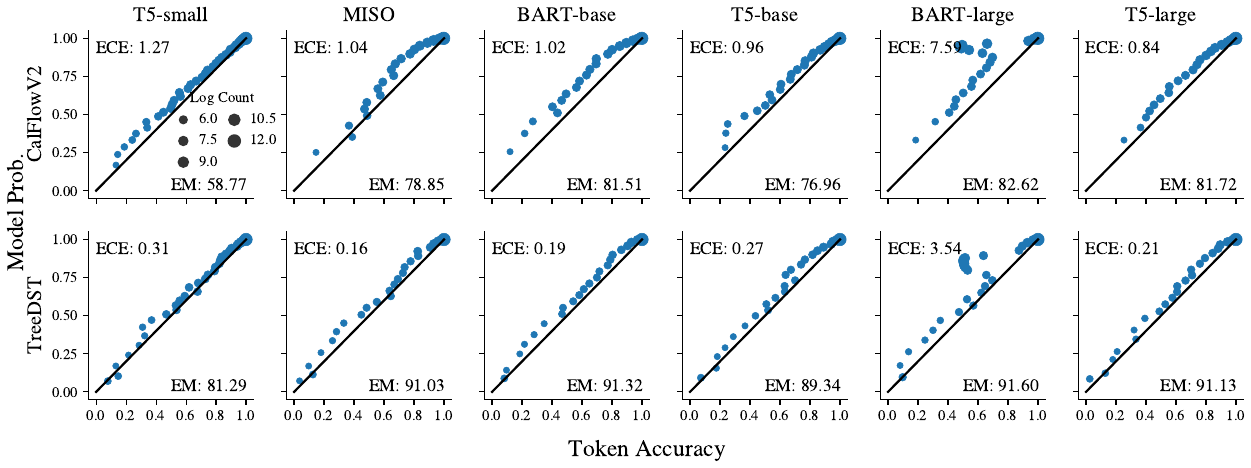
\includegraphics[width=3.363cm]{figures/img/hero_collage/tile_0.png}}};
\draw[black!35,line width=0.35pt] (0.070,-1.150) rectangle (3.433,-3.571);
\node[anchor=north west,text=ACMDarkBlue,font=\tiny\bfseries,inner sep=0] at (0.100,-3.601) {\href{https://arxiv.org/abs/2211.07443}{\adjustbox{max width=3.303cm}{Stengel-Eskin and Van Durme 2023}}};
\node[anchor=north west,text=black!60,font=\tiny,inner sep=0] at (0.100,-3.806) {\href{https://arxiv.org/abs/2211.07443}{Fig. 1, p.~6}};
\node[anchor=north west,inner sep=0] at (3.502,-1.150) {\href{https://arxiv.org/abs/2607.16799}{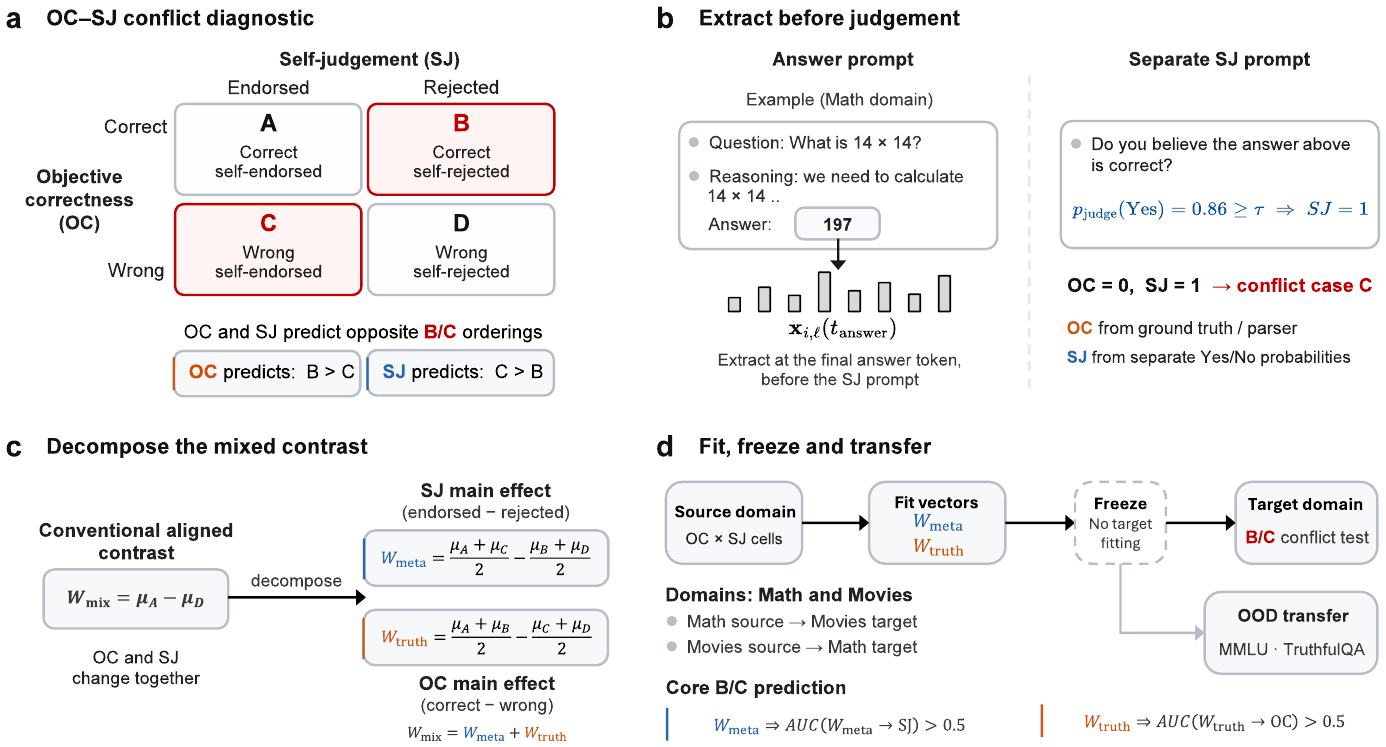
\includegraphics[width=3.363cm]{figures/img/hero_collage/tile_1.png}}};
\draw[black!35,line width=0.35pt] (3.502,-1.150) rectangle (6.865,-3.571);
\node[anchor=north west,text=ACMDarkBlue,font=\tiny\bfseries,inner sep=0] at (3.532,-3.601) {\href{https://arxiv.org/abs/2607.16799}{\adjustbox{max width=3.303cm}{Lu 2026}}};
\node[anchor=north west,text=black!60,font=\tiny,inner sep=0] at (3.532,-3.806) {\href{https://arxiv.org/abs/2607.16799}{Fig. 1, p.~2}};
\node[anchor=north west,inner sep=0] at (6.935,-1.150) {\href{https://arxiv.org/abs/2606.17234}{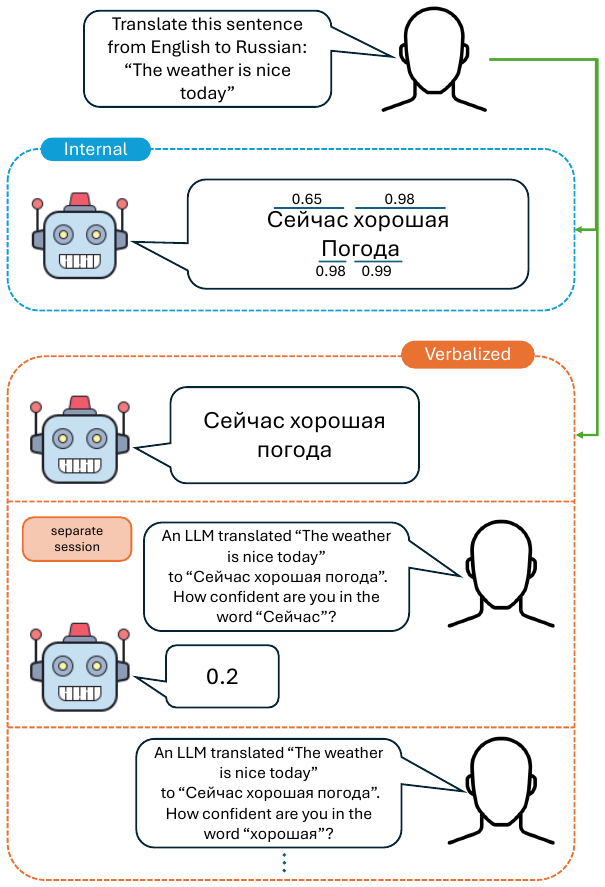
\includegraphics[width=3.363cm]{figures/img/hero_collage/tile_2.png}}};
\draw[black!35,line width=0.35pt] (6.935,-1.150) rectangle (10.298,-3.571);
\node[anchor=north west,text=ACMDarkBlue,font=\tiny\bfseries,inner sep=0] at (6.965,-3.601) {\href{https://arxiv.org/abs/2606.17234}{\adjustbox{max width=3.303cm}{Marashian et al. 2026}}};
\node[anchor=north west,text=black!60,font=\tiny,inner sep=0] at (6.965,-3.806) {\href{https://arxiv.org/abs/2606.17234}{Fig. 1, p.~1}};
\node[anchor=north west,inner sep=0] at (10.367,-1.150) {\href{https://arxiv.org/abs/2505.09427}{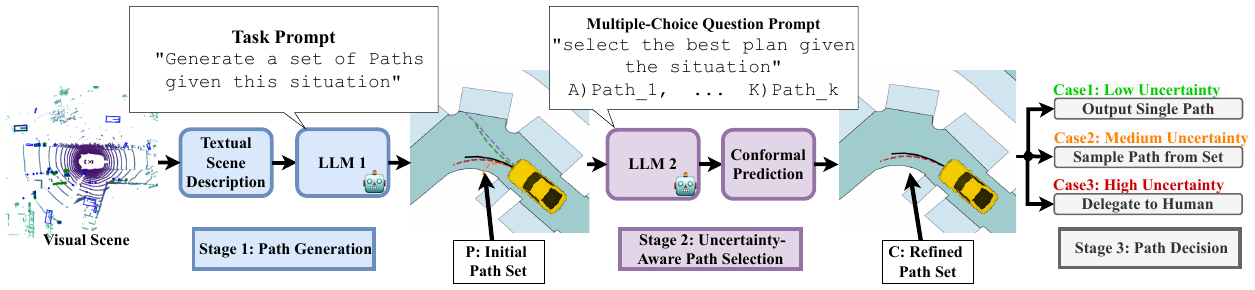
\includegraphics[width=3.363cm]{figures/img/hero_collage/tile_3.png}}};
\draw[black!35,line width=0.35pt] (10.367,-1.150) rectangle (13.730,-3.571);
\node[anchor=north west,text=ACMDarkBlue,font=\tiny\bfseries,inner sep=0] at (10.397,-3.601) {\href{https://arxiv.org/abs/2505.09427}{\adjustbox{max width=3.303cm}{Doula et al. 2025}}};
\node[anchor=north west,text=black!60,font=\tiny,inner sep=0] at (10.397,-3.806) {\href{https://arxiv.org/abs/2505.09427}{Fig. 1, p.~3}};
\fill[c7C5471] (0,-4.061) rectangle (13.800,-4.561);
\node[anchor=west,text=white,font=\footnotesize\bfseries,inner sep=0] at (0.14,-4.311) {Trained into the model: a calibration term in the training loss or reward (S4)};
\node[anchor=north west,inner sep=0] at (1.786,-4.631) {\href{https://arxiv.org/abs/2607.01612}{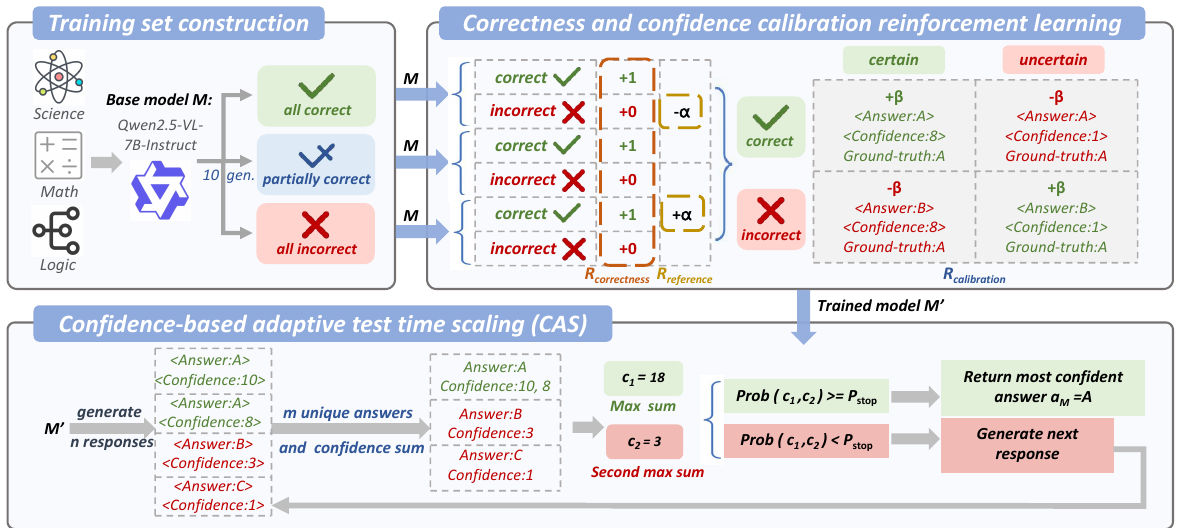
\includegraphics[width=3.363cm]{figures/img/hero_collage/tile_4.png}}};
\draw[black!35,line width=0.35pt] (1.786,-4.631) rectangle (5.149,-7.052);
\node[anchor=north west,text=ACMDarkBlue,font=\tiny\bfseries,inner sep=0] at (1.816,-7.082) {\href{https://arxiv.org/abs/2607.01612}{\adjustbox{max width=3.303cm}{Yang et al. 2026b}}};
\node[anchor=north west,text=black!60,font=\tiny,inner sep=0] at (1.816,-7.287) {\href{https://arxiv.org/abs/2607.01612}{Fig. 1, p.~3}};
\node[anchor=north west,inner sep=0] at (5.219,-4.631) {\href{https://arxiv.org/abs/2604.05306}{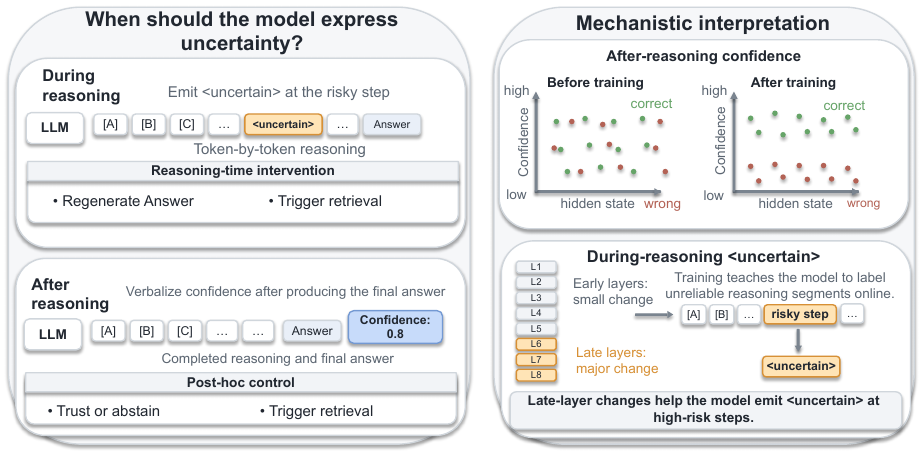
\includegraphics[width=3.363cm]{figures/img/hero_collage/tile_5.png}}};
\draw[black!35,line width=0.35pt] (5.219,-4.631) rectangle (8.581,-7.052);
\node[anchor=north west,text=ACMDarkBlue,font=\tiny\bfseries,inner sep=0] at (5.249,-7.082) {\href{https://arxiv.org/abs/2604.05306}{\adjustbox{max width=3.303cm}{Guo et al. 2026}}};
\node[anchor=north west,text=black!60,font=\tiny,inner sep=0] at (5.249,-7.287) {\href{https://arxiv.org/abs/2604.05306}{Fig. 1, p.~2}};
\node[anchor=north west,inner sep=0] at (8.651,-4.631) {\href{https://arxiv.org/abs/2604.22779}{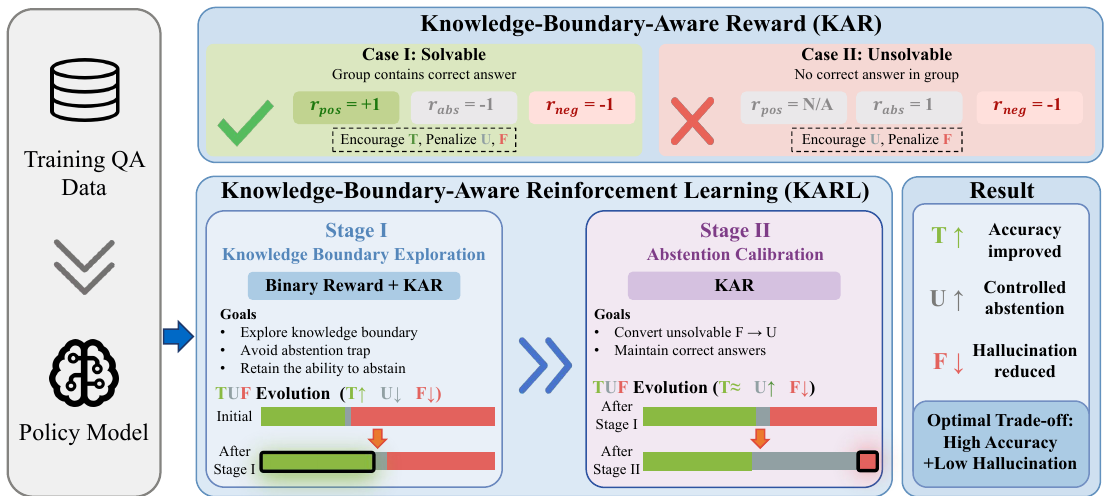
\includegraphics[width=3.363cm]{figures/img/hero_collage/tile_6.png}}};
\draw[black!35,line width=0.35pt] (8.651,-4.631) rectangle (12.014,-7.052);
\node[anchor=north west,text=ACMDarkBlue,font=\tiny\bfseries,inner sep=0] at (8.681,-7.082) {\href{https://arxiv.org/abs/2604.22779}{\adjustbox{max width=3.303cm}{Gao et al. 2026}}};
\node[anchor=north west,text=black!60,font=\tiny,inner sep=0] at (8.681,-7.287) {\href{https://arxiv.org/abs/2604.22779}{Fig. 4, p.~4}};
\end{tikzpicture}}
\caption{\textbf{Confidence estimated after the fact, and confidence trained into the model.} Panels are drawn from Figures~\ref{fig:method_gallery} and~\ref{fig:results_gallery} under the same licence rule: one per stage for S0, S1, S2, S3, and one per training family for S4 (T1, T3, T4; T2, T5 not shown). Each label links to the paper; Table~\ref{tab:panel_provenance} gives the figure, page and licence.}
\Description{A labelled grid of images, each a hyperlink annotated with its system name and source figure number.}
\label{fig:hero_collage}
\end{figure*}



This survey maps calibration-aware decision-making with language models, with the training stage as
its core. We place each of \nWorks works by the stage at which calibration enters the decision
pipeline (Table~\ref{tab:definitions}), organise the \nCore training-stage works by what the training
signal scores, and classify every work by the \emph{output contract} its confidence is attached to:
a typed decision with a probability per declared option, a prediction set, constrained output, a single
confidence score, or free text. The two classifications meet in one finding: of the \nContractTyped works
that attach the confidence to a typed decision, most calibrate a classifier or a multiple-choice
read-off after the fact, and only \nCoreTyped of the \nCore training works train one
(Section~\ref{sec:contract}).

\paragraph{Contributions.} This survey offers the following.
\begin{itemize}
  \item A \textbf{stage taxonomy} of \nWorks works (Figure~\ref{fig:taxonomy_main} shows \nTaxShown of them), with operational
        placement rules (Table~\ref{tab:definitions}) and a per-work record of stage, output contract,
        access, guarantee, metric and action (Tables~\ref{tab:compare_s4} and~\ref{tab:landscape}).
  \item A \textbf{typology of calibration training}: the \nCore training-stage works in five families
        by what the training signal scores (Section~\ref{sec:core}, Table~\ref{tab:compare_s4}), and
        what each stage yields, costs and guarantees (Table~\ref{tab:stage_limits}).
  \item A \textbf{coverage comparison} with the \nSurveysCompared closest prior surveys
        (Table~\ref{tab:survey_compare}, Figure~\ref{fig:survey_timeline}), and a profile of the corpus
        (Figures~\ref{fig:corpus_overview} to~\ref{fig:results_gallery}), every gallery panel
        traced to its source figure and licence (Table~\ref{tab:panel_provenance}).
  \item An analysis of the \textbf{output contract and the decision loop} (Section~\ref{sec:contract},
        Figure~\ref{fig:decision_loop}, Table~\ref{tab:compare_contract}).
  \item A \textbf{measurable agenda}: seven quantities with named public testbeds
        (Table~\ref{tab:future_metrics}), with the calibration of the decision itself measured for the
        \nDISystems systems of a public leaderboard (Figure~\ref{fig:future_protocol}).
\end{itemize}

% AUTO-GENERATED by build/gen_taxonomy.py from literature/corpus.tsv -- do not hand-edit.
\begin{figure*}[p]
\centering
\resizebox{!}{0.84\textheight}{%
\begin{forest}
  for tree={align=center},
  where n children=0{font=\footnotesize, align=left}{font=\normalsize},
  where level=1{font=\large}{},
  where level=0{font=\Large}{},
[\textbf{Calibration-aware}\\\textbf{decision-making}\\\textbf{with language}\\\textbf{models}, fill=black!8, text width=12em
  [\textbf{S0 read-off}, fill=stS0!40, text width=9em
    [\textbf{Calibration after}\\\textbf{alignment}, fill=stS0!22, text width=12.5em
      [{\textbf{OpenAI}: GPT-4 Technical Report~\citep{openai2023gpt4}\\\textbf{Sanz-Guerrero}: Large Language Models Are\ldots~\citep{sanzguerrero2026large}}, fill=stS0!7, text width=40em, align=left]
    ]
    [\textbf{Empirical studies of}\\\textbf{read-off calibration}, fill=stS0!22, text width=12.5em
      [{\textbf{Desai}: Calibration of Pre-trained Transformers~\citep{desai2020calibration}\\\textbf{Calibration Across Layers}: Understanding Calibration\ldots~\citep{joshi2025calibration}}, fill=stS0!7, text width=40em, align=left]
    ]
    [\textbf{Likelihood and logit}\\\textbf{read-off}, fill=stS0!22, text width=12.5em
      [{\textbf{Ott}: Analyzing Uncertainty in Neural Machine Translation~\citep{ott2018analyzing}\\\textbf{My Answer is C}: First-Token Probabilities Do Not Match\ldots~\citep{wang2024my}}, fill=stS0!7, text width=40em, align=left]
    ]
    [\textbf{Self-evaluation and}\\\textbf{read-off calibration}, fill=stS0!22, text width=12.5em
      [{\textbf{Kadavath}: Language Models (Mostly) Know What They Know~\citep{kadavath2022language}}, fill=stS0!7, text width=40em, align=left]
    ]
  ]
  [\textbf{S1 post-hoc}\\\textbf{map}, fill=stS1!40, text width=9em
    [\textbf{Fixed maps over the}\\\textbf{read-off}, fill=stS1!22, text width=12.5em
      [{\textbf{Zhang}: Enhancing Uncertainty-Based Hallucination Detection\ldots~\citep{zhang2023enhancing}\\\textbf{The Silent Vote}: Improving Zero-Shot LLM Reliability by\ldots~\citep{badhe2026silent}}, fill=stS1!7, text width=40em, align=left]
    ]
    [\textbf{Label-bias and}\\\textbf{option-prior}\\\textbf{debiasing}, fill=stS1!22, text width=12.5em
      [{\textbf{Zheng}: Large Language Models Are Not Robust Multiple Choice\ldots~\citep{zheng2023large}\\\textbf{Beyond Performance}: Quantifying and Mitigating Label Bias\ldots~\citep{reif2024beyond}}, fill=stS1!7, text width=40em, align=left]
    ]
    [\textbf{Learned calibrators}, fill=stS1!22, text width=12.5em
      [{\textbf{Ye}: Can Explanations Be Useful for Calibrating Black Box Models?~\citep{ye2021can}\\\textbf{Luo}: Unlocking the Pre-Trained Model as a Dual-Alignment\ldots~\citep{luo2026unlocking}}, fill=stS1!7, text width=40em, align=left]
    ]
    [\textbf{Multicalibration and}\\\textbf{task-specific}\\\textbf{recalibration}, fill=stS1!22, text width=12.5em
      [{\textbf{Detommaso}: Multicalibration for Confidence Scoring in\ldots~\citep{detommaso2024multicalibration}\\\textbf{Liu}: On Calibration of LLM-based Guard Models for Reliable\ldots~\citep{liu2024calibration}}, fill=stS1!7, text width=40em, align=left]
    ]
    [\textbf{Probes and learned}\\\textbf{confidence heads}, fill=stS1!22, text width=12.5em
      [{\textbf{Kumar}: Calibration of Encoder Decoder Models for Neural\ldots~\citep{kumar2019calibration}\\\textbf{Lu}: Diagnosing Correctness Probes under Self-Judgement\ldots~\citep{lu2026diagnosing}}, fill=stS1!7, text width=40em, align=left]
    ]
    [\textbf{Prompt and context}\\\textbf{calibration}, fill=stS1!22, text width=12.5em
      [{\textbf{Surface Form Competition}: Why the Highest Probability\ldots~\citep{holtzman2021surface}\\\textbf{Gundem}: Boosting In-Context Learning in LLMs Through the\ldots~\citep{gundem2025boosting}}, fill=stS1!7, text width=40em, align=left]
    ]
    [\textbf{Scaling and binning}, fill=stS1!22, text width=12.5em
      [{\textbf{Guo}: On Calibration of Modern Neural Networks~\citep{guo2017calibration}\\\textbf{Luo}: Your Pre-trained LLM is Secretly an Unsupervised\ldots~\citep{luo2025your}}, fill=stS1!7, text width=40em, align=left]
    ]
  ]
  [\textbf{S2 prompt}\\\textbf{elicitation}, fill=stS2!40, text width=9em
    [\textbf{Abstention prompting}, fill=stS2!22, text width=12.5em
      [{\textbf{I-CALM}: Incentivizing Confidence-Aware Abstention for LLM\ldots~\citep{zong2026icalm}}, fill=stS2!7, text width=40em, align=left]
    ]
    [\textbf{Introspection,}\\\textbf{deliberation and}\\\textbf{task-specific}\\\textbf{elicitation}, fill=stS2!22, text width=12.5em
      [{\textbf{Sun}: Confidence Estimation for LLM-Based Dialogue State Tracking~\citep{sun2024confidence}\\\textbf{Reasoning about Uncertainty}: Do Reasoning Models Know\ldots~\citep{mei2025reasoning}}, fill=stS2!7, text width=40em, align=left]
    ]
    [\textbf{Linguistic hedges and}\\\textbf{epistemic markers}, fill=stS2!22, text width=12.5em
      [{\textbf{Sileo}: Probing neural language models for understanding of\ldots~\citep{sileo2022probing}\\\textbf{Liu}: Can LLMs Use Linguistic Uncertainty Markers to Reliably\ldots~\citep{liu2026can}}, fill=stS2!7, text width=40em, align=left]
    ]
    [\textbf{Self-evaluation}\\\textbf{prompts}, fill=stS2!22, text width=12.5em
      [{\textbf{Tian}: Overconfidence in LLM-as-a-Judge: Diagnosis and\ldots~\citep{tian2025overconfidence}}, fill=stS2!7, text width=40em, align=left]
    ]
    [\textbf{Stated confidence}\\\textbf{that triggers an}\\\textbf{action}, fill=stS2!22, text width=12.5em
      [{\textbf{Ni}: When Do LLMs Need Retrieval Augmentation? Mitigating LLMs'\ldots~\citep{ni2024when}\\\textbf{Ferrer}: When Can We Trust LLM Graders? Calibrating\ldots~\citep{ferrer2026when}}, fill=stS2!7, text width=40em, align=left]
    ]
    [\textbf{Verbalised numeric}\\\textbf{confidence}, fill=stS2!22, text width=12.5em
      [{\textbf{Tanneru}: Quantifying Uncertainty in Natural Language\ldots~\citep{tanneru2023quantifying}\\\textbf{Yang}: The Mirage of Calibrated Confidence\ldots~\citep{yang2026the}}, fill=stS2!7, text width=40em, align=left]
    ]
  ]
  [\textbf{S3 extra}\\\textbf{inference}, fill=stS3!40, text width=9em
    [\textbf{Benchmarks and}\\\textbf{empirical studies}, fill=stS3!22, text width=12.5em
      [{\textbf{LM-Polygraph}: Uncertainty Estimation for Language Models~\citep{fadeeva2023lmpolygraph}\\\textbf{Vashurin}: Benchmarking Uncertainty Quantification\ldots~\citep{vashurin2024benchmarking}}, fill=stS3!7, text width=40em, align=left]
    ]
    [\textbf{Conformal abstention,}\\\textbf{selection and}\\\textbf{cascades}, fill=stS3!22, text width=12.5em
      [{\textbf{Fisch}: Efficient Conformal Prediction via Cascaded\ldots~\citep{fisch2020efficient}\\\textbf{Tayebati}: Learning Conformal Abstention Policies for\ldots~\citep{tayebati2025learning}}, fill=stS3!7, text width=40em, align=left]
    ]
    [\textbf{Conformal factuality}\\\textbf{and claim filtering}, fill=stS3!22, text width=12.5em
      [{\textbf{Cherian}: Large language model validity via enhanced\ldots~\citep{cherian2024large}\\\textbf{Rubin-Toles}: Conformal Language Model Reasoning with\ldots~\citep{rubintoles2025conformal}}, fill=stS3!7, text width=40em, align=left]
    ]
    [\textbf{Conformal prediction}\\\textbf{sets}, fill=stS3!22, text width=12.5em
      [{\textbf{Dey}: Conformal prediction for text infilling and\ldots~\citep{dey2021conformal}\\\textbf{CommCP}: Efficient Multi-Agent Coordination via LLM-Based\ldots~\citep{zhang2026commcp}}, fill=stS3!7, text width=40em, align=left]
    ]
    [\textbf{Ensembles and}\\\textbf{cross-model}\\\textbf{disagreement}, fill=stS3!22, text width=12.5em
      [{\textbf{Dong}: Confidence Modeling for Neural Semantic Parsing~\citep{dong2018confidence}\\\textbf{Hamidieh}: Complementing Self-Consistency with\ldots~\citep{hamidieh2026complementing}}, fill=stS3!7, text width=40em, align=left]
    ]
    [\textbf{Internal-state}\\\textbf{signals}, fill=stS3!22, text width=12.5em
      [{\textbf{Fomicheva}: Unsupervised Quality Estimation for Neural\ldots~\citep{fomicheva2020unsupervised}\\\textbf{Semantic Volume}: Quantifying and Detecting both External and\ldots~\citep{li2025semantic}}, fill=stS3!7, text width=40em, align=left]
    ]
    [\textbf{Long-form and}\\\textbf{claim-level}, fill=stS3!22, text width=12.5em
      [{\textbf{Da}: LLM Uncertainty Quantification through Directional\ldots~\citep{da2024llm}\\\textbf{IUQ}: Interrogative Uncertainty Quantification for Long-Form\ldots~\citep{fan2026iuq}}, fill=stS3!7, text width=40em, align=left]
    ]
    [\textbf{Risk control and}\\\textbf{early exit}, fill=stS3!22, text width=12.5em
      [{\textbf{Learn then Test}: Calibrating Predictive Algorithms\ldots~\citep{angelopoulos2021learn}\\\textbf{Conformal Thinking}: Risk Control for Reasoning on a\ldots~\citep{wang2026conformal}}, fill=stS3!7, text width=40em, align=left]
    ]
    [\textbf{Sampling consistency}, fill=stS3!22, text width=12.5em
      [{\textbf{Wang}: Self-Consistency Improves Chain of Thought Reasoning\ldots~\citep{wang2022selfconsistency}\\\textbf{Too Consistent to Detect}: A Study of Self-Consistent\ldots~\citep{tan2025too}}, fill=stS3!7, text width=40em, align=left]
    ]
    [\textbf{Semantic entropy and}\\\textbf{meaning clustering}, fill=stS3!22, text width=12.5em
      [{\textbf{Semantic Uncertainty}: Linguistic Invariances for\ldots~\citep{kuhn2023semantic}\\\textbf{Sun}: Efficient Hallucination Detection: Adaptive Bayesian\ldots~\citep{sun2026efficient}}, fill=stS3!7, text width=40em, align=left]
    ]
    [\textbf{Token-level}\\\textbf{aggregation}, fill=stS3!22, text width=12.5em
      [{\textbf{Malinin}: Uncertainty Estimation in Autoregressive\ldots~\citep{malinin2020uncertainty}\\\textbf{Word-Sequence Entropy}: Towards Uncertainty Estimation in\ldots~\citep{wang2024wordsequence}}, fill=stS3!7, text width=40em, align=left]
    ]
  ]
  [\textbf{S4 training}, fill=stS4!40, text width=9em
    [\textbf{T1 supervised}\\\textbf{calibration}\\\textbf{objectives}, fill=stS4!30, text width=10.5em
      [{\textbf{Jiang}: How Can We Know When Language Models Know? On the\ldots~\citep{jiang2020how}\\\textbf{Chaudhry}: Finetuning Language Models to Emit Linguistic\ldots~\citep{chaudhry2024finetuning}\\\textbf{Kapoor}: Large Language Models Must Be Taught to Know What\ldots~\citep{kapoor2024large}\\\textbf{Niu}: Functional-level Uncertainty Quantification for\ldots~\citep{niu2024functionallevel}\\\textbf{Uncertainty Distillation}: Teaching Language Models to\ldots~\citep{hager2025uncertainty}\\\textbf{ConfTuner}: Training Large Language Models to Express Their\ldots~\citep{li2025conftuner}\\\textbf{Direct Confidence Alignment}: Aligning Verbalized\ldots~\citep{zhang2025direct}\\\textbf{Know When You're Wrong}: Aligning Confidence with\ldots~\citep{xiaohu2026know}}, fill=stS4!8, text width=40em, align=left]
    ]
    [\textbf{T2 reward-model}\\\textbf{calibration}, fill=stS4!30, text width=10.5em
      [{\textbf{Leng}: Taming Overconfidence in LLMs: Reward Calibration in RLHF~\citep{leng2024taming}\\\textbf{Lou}: Uncertainty-aware Reward Model: Teaching Reward Models\ldots~\citep{lou2024uncertaintyaware}\\\textbf{Know What You Don't Know}: Uncertainty Calibration of\ldots~\citep{park2025know}\\\textbf{Ma}: Distributional Process Reward Models: Calibrated\ldots~\citep{ma2026distributional}\\\textbf{Pan}: Uncertainty-Aware Reward Modeling for Stable RLHF~\citep{pan2026uncertaintyaware}}, fill=stS4!8, text width=40em, align=left]
    ]
    [\textbf{T3 calibration}\\\textbf{rewards on the}\\\textbf{stated confidence}, fill=stS4!30, text width=10.5em
      [{\textbf{Band}: Linguistic Calibration of Long-Form Generations~\citep{band2024linguistic}\\\textbf{Rewarding Doubt}: A Reinforcement Learning Approach\ldots~\citep{baniharouni2025rewarding}\\\textbf{Niekerk}: Post-Training Large Language Models via\ldots~\citep{vanniekerk2025posttraining}\\\textbf{Zou}: Thinking, Faithful and Stable: Mitigating Hallucinations\ldots~\citep{zou2025thinking}\\\textbf{ORCE}: Order-Aware Alignment of Verbalized Confidence in Large\ldots~\citep{li2026orce}\\\textbf{Singh}: Verifiable Rewards for Calibrated Probabilistic\ldots~\citep{singh2026verifiable}\\\textbf{DualStake}: Dual-Path Confidence Calibration in Deep Research\ldots~\citep{xu2026dualstake}\\\textbf{Closing the Reflection Gap}: A Free Calibration Bonus for\ldots~\citep{zhu2026closing}}, fill=stS4!8, text width=40em, align=left]
    ]
    [\textbf{T4 abstention and}\\\textbf{refusal training}, fill=stS4!30, text width=10.5em
      [{\textbf{Yang}: Alignment for Honesty~\citep{yang2023alignment}\\\textbf{Chen}: Teaching Large Language Models to Express Knowledge\ldots~\citep{chen2024teaching}\\\textbf{Know the Unknown}: An Uncertainty-Sensitive Method for LLM\ldots~\citep{li2024know}\\\textbf{Xu}: Rejection Improves Reliability: Training LLMs to Refuse\ldots~\citep{xu2024rejection}\\\textbf{Honesty over Accuracy}: Trustworthy Language Models\ldots~\citep{mohamadi2025honesty}\\\textbf{TruthRL}: Incentivizing Truthful LLMs via Reinforcement Learning~\citep{wei2025truthrl}\\\textbf{TIAR}: Trajectory-Informed Advantage Reweighting for LLM\ldots~\citep{pan2026tiar}\\\textbf{Abstain-R1}: Calibrated Abstention and Post-Refusal\ldots~\citep{zhai2026abstainr1}}, fill=stS4!8, text width=40em, align=left]
    ]
    [\textbf{T5 process- and}\\\textbf{meaning-level}\\\textbf{confidence rewards}, fill=stS4!30, text width=10.5em
      [{\textbf{An}: Teaching LLMs to Abstain via Fine-Grained Semantic\ldots~\citep{an2025teaching}\\\textbf{MMBoundary}: Advancing MLLM Knowledge Boundary Awareness\ldots~\citep{he2025mmboundary}\\\textbf{Wang}: Process Supervision of Confidence Margin for\ldots~\citep{wang2026process}\\\textbf{Yu}: Calibrating LLMs with Semantic-level Reward~\citep{yu2026calibrating}}, fill=stS4!8, text width=40em, align=left]
    ]
  ]
  [\textbf{Theory and}\\\textbf{analysis}, fill=stTH!40, text width=9em
    [{\textbf{Błasiok}: When Does Optimizing a Proper Loss Yield\ldots~\citep{blasiok2023when}\\\textbf{Kalai}: Calibrated Language Models Must Hallucinate~\citep{kalai2023calibrated}\\\textbf{Uncalibrated Reasoning}: GRPO Induces Overconfidence\ldots~\citep{bereket2025uncalibrated}\\\textbf{Kalai}: Why Language Models Hallucinate~\citep{kalai2025why}\\\textbf{Nakkiran}: Trained on Tokens, Calibrated on Concepts\ldots~\citep{nakkiran2025trained}}, fill=stTH!15, text width=40em, align=left]
  ]
  [\textbf{X consumers}\\\textbf{and contract}, fill=stX!40, text width=9em
    [\textbf{Abstention}, fill=stX!22, text width=12.5em
      [{\textbf{Kamath}: Selective Question Answering under Domain Shift~\citep{kamath2020selective}\\\textbf{Srinivasan}: Selective "Selective Prediction"\ldots~\citep{srinivasan2024selective}}, fill=stX!7, text width=40em, align=left]
    ]
    [\textbf{Adaptive compute}, fill=stX!22, text width=12.5em
      [{\textbf{Let's Sample Step by Step}: Adaptive-Consistency for\ldots~\citep{aggarwal2023lets}\\\textbf{Yang}: Dynamic Early Exit in Reasoning Models~\citep{yang2025dynamic}}, fill=stX!7, text width=40em, align=left]
    ]
    [\textbf{Confidence-weighted}\\\textbf{selection}, fill=stX!22, text width=12.5em
      [{\textbf{Taubenfeld}: Confidence Improves Self-Consistency in LLMs~\citep{taubenfeld2025confidence}}, fill=stX!7, text width=40em, align=left]
    ]
    [\textbf{Constrained decoding}, fill=stX!22, text width=12.5em
      [{\textbf{PICARD}: Parsing Incrementally for Constrained\ldots~\citep{scholak2021picard}\\\textbf{Reddy}: The Hidden Cost of Structured Generation in LLMs\ldots~\citep{reddy2026hidden}}, fill=stX!7, text width=40em, align=left]
    ]
    [\textbf{Deferral}, fill=stX!22, text width=12.5em
      [{\textbf{Jitkrittum}: When Does Confidence-Based Cascade\ldots~\citep{jitkrittum2023when}\\\textbf{L2D-Clinical}: Learning to Defer for Adaptive Model\ldots~\citep{kondadadi2026l2dclinical}}, fill=stX!7, text width=40em, align=left]
    ]
    [\textbf{Human reliance on}\\\textbf{model output and}\\\textbf{stated confidence}, fill=stX!22, text width=12.5em
      [{\textbf{Si}: Large Language Models Help Humans Verify Truthfulness --\ldots~\citep{si2023large}\\\textbf{Not All Uncertainty Is Equal}: How Uncertainty\ldots~\citep{villavicencio2026not}}, fill=stX!7, text width=40em, align=left]
    ]
    [\textbf{Judge calibration}, fill=stX!22, text width=12.5em
      [{\textbf{Liu}: Calibrating LLM-Based Evaluator~\citep{liu2023calibrating}\\\textbf{JEV-as-a-Judge}: Accept When Confident, Escalate When Unsure~\citep{li2026jev}}, fill=stX!7, text width=40em, align=left]
    ]
    [\textbf{Routing/cascade}, fill=stX!22, text width=12.5em
      [{\textbf{Model Cascading}: Towards Jointly Improving Efficiency\ldots~\citep{varshney2022model}\\\textbf{Bouchard}: Is Escalation Worth It? A Decision-Theoretic\ldots~\citep{bouchard2026is}}, fill=stX!7, text width=40em, align=left]
    ]
    [\textbf{Structured-output}\\\textbf{benchmark}, fill=stX!22, text width=12.5em
      [{\textbf{Struc-Bench}: Are Large Language Models Really Good at\ldots~\citep{tang2023strucbench}\\\textbf{Singh}: The Structured Output Benchmark: A Multi-Source\ldots~\citep{singh2026structured}}, fill=stX!7, text width=40em, align=left]
    ]
    [\textbf{Studies and}\\\textbf{benchmarks of}\\\textbf{abstention}, fill=stX!22, text width=12.5em
      [{\textbf{Tomani}: Uncertainty-Based Abstention in LLMs Improves\ldots~\citep{tomani2024uncertaintybased}\\\textbf{Wang}: Are LLM Decisions Faithful to Verbal Confidence?~\citep{wang2026are}}, fill=stX!7, text width=40em, align=left]
    ]
    [\textbf{Typed classification}, fill=stX!22, text width=12.5em
      [{\textbf{Look at the Text}: Instruction-Tuned Language Models are\ldots~\citep{wang2024look}}, fill=stX!7, text width=40em, align=left]
    ]
  ]
]
\end{forest}}
\caption{\textbf{A taxonomy of calibration-aware decision-making with language models} (111 of the 408
works in Tables~\ref{tab:compare_s4} and~\ref{tab:landscape}). Branches are the stage at which calibration enters (Table~\ref{tab:definitions}); X holds
the works that consume a confidence or fix the output contract. The core, S4 (80 works), is grouped by what the
training signal scores and lists up to 8 works per family, evenly spaced over the family's works in year order
(33 shown; all are in Table~\ref{tab:compare_s4}). The 5 theory and analysis works are listed in
full and are not counted in the core. Every other family lists its earliest and its latest work. Each line gives a trimmed form
of the paper's own title; a citation may show a later venue year than the first-version year counted in
Figures~\ref{fig:corpus_dist} and~\ref{fig:stage_trend}.}
\Description{A tree diagram rooted at calibration-aware decision-making with language models, with branches for read-off,
post-hoc maps, prompt elicitation, extra inference, training (split into five families by what the training signal scores),
theory and analysis, and consumers and output contract. Each family cell lists papers with short titles.}
\label{fig:taxonomy_main}
\end{figure*}


\subsection{Related surveys and the empty cell}
\label{sec:related}

Table~\ref{tab:survey_compare} (Appendix~\ref{app:surveys}) compares the \nSurveysCompared closest prior surveys on seven topics:
confidence estimation and calibration, calibration-aware training of any kind, reinforcement learning
whose reward is a calibration or proper-scoring-rule objective, decisions over a predefined option set,
typed per-option decision outputs, acting on confidence, and hallucination.
Figure~\ref{fig:survey_timeline} places them on a timeline; \nSurveysRecent of the \nSurveysCompared
appeared from 2024 onward.


Calibration and uncertainty are well surveyed, and the stage view itself, which organises methods by
where the confidence comes from, is established~\citep{li2025survey,shorinwa2025survey}; we use it as
the frame for the background stages and credit it there. The training stage is the thinner cell. Only
\nRLRFull surveys give full coverage to reinforcement learning with a calibration reward, and each is
scoped to one slice: \citet{li2025survey} to the 2024 methods, \citet{xu2026llm} to forecasting, where
it organises calibration training by reward and maps forecast forms to proper scores, and
\citet{lin2026uncertainty} to agents, where it splits rewards by their target. \citet{ulmer2025anthropomimetic}
labels papers by the register of the confidence, numeric or verbal, and by how it is elicited: by prompting,
supervised fine-tuning or reinforcement learning. What none of the \nSurveys
surveys we identified does is organise calibration training \emph{across domains} by what the training signal scores,
or cross that typology with the output contract the confidence is trained into; no survey cites more
than one of the \nCoreFourteen general-domain calibration-training works from 2025 and 2026 that anchor
our core (marked in Table~\ref{tab:compare_s4}). Two recent non-survey works come closest: an application
paper that compares reinforcement-learning training paradigms by their signal source for one
domain~\citep{barbosa2026calibrated}, and a position paper that groups ternary-reward abstention works, three of them in
our core, in one row~\citep{ravikumar2026missing}; neither proposes a typology of training signals or an output contract. Typed per-option decision output is the emptiest column of Table~\ref{tab:survey_compare}:
no survey covers it in full.

% AUTO-GENERATED by build/gen_phaseA.py -- do not hand-edit.
\begin{figure*}[t]
\centering
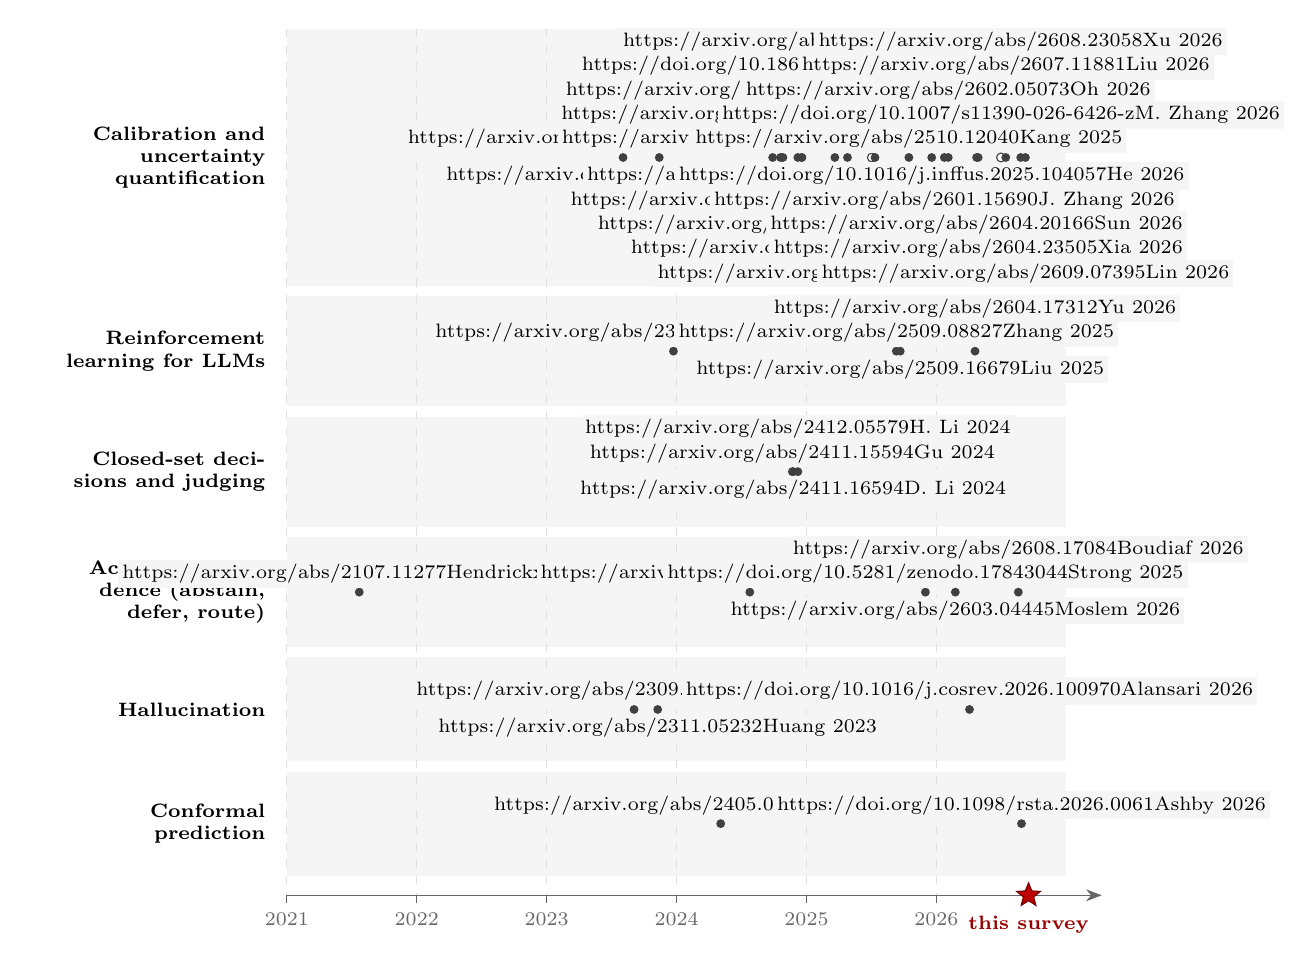
\begin{tikzpicture}[font=\scriptsize]
\fill[black!4] (0,1.63) rectangle (9.90,-1.63);
\fill[black!4] (0,-1.76) rectangle (9.90,-3.16);
\fill[black!4] (0,-3.29) rectangle (9.90,-4.69);
\fill[black!4] (0,-4.82) rectangle (9.90,-6.22);
\fill[black!4] (0,-6.35) rectangle (9.90,-7.67);
\fill[black!4] (0,-7.80) rectangle (9.90,-9.12);
\draw[black!12,dashed] (0.00,1.63) -- (0.00,-9.37);
\draw[black!12,dashed] (1.65,1.63) -- (1.65,-9.37);
\draw[black!12,dashed] (3.30,1.63) -- (3.30,-9.37);
\draw[black!12,dashed] (4.95,1.63) -- (4.95,-9.37);
\draw[black!12,dashed] (6.60,1.63) -- (6.60,-9.37);
\draw[black!12,dashed] (8.25,1.63) -- (8.25,-9.37);
\node[anchor=east,align=right,text width=2.9cm,font=\scriptsize\bfseries] at (-0.15,0.00) {Calibration and uncertainty quantification};
\draw[black!35] (6.27,0.00) -- (6.27,0.36);
\draw[black!35] (6.30,0.00) -- (6.30,-0.36);
\draw[black!35] (6.49,0.00) -- (6.49,0.67);
\draw[black!35] (6.54,0.00) -- (6.54,-0.67);
\draw[black!35] (7.43,0.00) -- (7.43,0.98);
\draw[black!35] (6.96,0.00) -- (6.96,-0.98);
\draw[black!35] (7.12,0.00) -- (7.12,1.29);
\draw[black!35] (7.47,0.00) -- (7.47,-1.29);
\draw[black!35] (9.07,0.00) -- (9.07,0.36);
\draw[black!35] (8.35,0.00) -- (8.35,-0.36);
\draw[black!35] (8.40,0.00) -- (8.40,0.67);
\draw[black!35] (8.76,0.00) -- (8.76,-0.67);
\draw[black!35] (8.78,0.00) -- (8.78,-0.98);
\draw[black!35] (9.13,0.00) -- (9.13,0.98);
\draw[black!35] (9.32,0.00) -- (9.32,1.29);
\draw[black!35] (9.38,0.00) -- (9.38,-1.29);
\fill[black!75] (4.27,0.00) circle (1.6pt);
\node[anchor=south,inner sep=1.5pt,fill=black!4] at (4.27,0.05) {\href{https://arxiv.org/abs/2308.01222}{Wang 2023}};
\fill[black!75] (4.73,0.00) circle (1.6pt);
\node[anchor=north,inner sep=1.5pt,fill=black!4] at (4.73,-0.05) {\href{https://arxiv.org/abs/2311.08298}{Geng 2023}};
\fill[black!75] (6.17,0.00) circle (1.6pt);
\node[anchor=south,inner sep=1.5pt,fill=black!4] at (6.17,0.05) {\href{https://arxiv.org/abs/2409.18786}{S. Li 2024}};
\fill[black!75] (6.27,0.00) circle (1.6pt);
\node[anchor=south,inner sep=1.5pt,fill=black!4] at (6.27,0.36) {\href{https://arxiv.org/abs/2410.15326}{Huang 2024}};
\fill[black!75] (6.30,0.00) circle (1.6pt);
\node[anchor=north,inner sep=1.5pt,fill=black!4] at (6.30,-0.36) {\href{https://arxiv.org/abs/2410.20199}{Beigi 2024}};
\fill[black!75] (6.49,0.00) circle (1.6pt);
\node[anchor=south,inner sep=1.5pt,fill=black!4] at (6.49,0.67) {\href{https://arxiv.org/abs/2412.05563}{Shorinwa 2024}};
\fill[black!75] (6.54,0.00) circle (1.6pt);
\node[anchor=north,inner sep=1.5pt,fill=black!4] at (6.54,-0.05) {\href{https://arxiv.org/abs/2412.12472}{M. Li 2024}};
\fill[black!75] (6.54,0.00) circle (1.6pt);
\node[anchor=north,inner sep=1.5pt,fill=black!4] at (6.54,-0.67) {\href{https://arxiv.org/abs/2412.12767}{Xie 2024}};
\draw[black!75,fill=white] (7.43,0.00) circle (1.6pt);
\node[anchor=south,inner sep=1.5pt,fill=black!4] at (7.43,0.98) {\href{https://doi.org/10.18653/v1/2025.findings-acl.1101}{Xia 2025}};
\fill[black!75] (6.96,0.00) circle (1.6pt);
\node[anchor=north,inner sep=1.5pt,fill=black!4] at (6.96,-0.98) {\href{https://arxiv.org/abs/2503.15850}{Liu 2025}};
\fill[black!75] (7.12,0.00) circle (1.6pt);
\node[anchor=south,inner sep=1.5pt,fill=black!4] at (7.12,1.29) {\href{https://arxiv.org/abs/2504.18346}{Abbasli 2025}};
\fill[black!75] (7.47,0.00) circle (1.6pt);
\node[anchor=north,inner sep=1.5pt,fill=black!4] at (7.47,-1.29) {\href{https://arxiv.org/abs/2507.10587}{Ulmer 2025}};
\fill[black!75] (7.90,0.00) circle (1.6pt);
\node[anchor=south,inner sep=1.5pt,fill=black!4] at (7.90,0.05) {\href{https://arxiv.org/abs/2510.12040}{Kang 2025}};
\fill[black!75] (8.19,0.00) circle (1.6pt);
\node[anchor=north,inner sep=1.5pt,fill=black!4] at (8.19,-0.05) {\href{https://doi.org/10.1016/j.inffus.2025.104057}{He 2026}};
\draw[black!75,fill=white] (9.07,0.00) circle (1.6pt);
\node[anchor=south,inner sep=1.5pt,fill=black!4] at (9.07,0.36) {\href{https://doi.org/10.1007/s11390-026-6426-z}{M. Zhang 2026}};
\fill[black!75] (8.35,0.00) circle (1.6pt);
\node[anchor=north,inner sep=1.5pt,fill=black!4] at (8.35,-0.36) {\href{https://arxiv.org/abs/2601.15690}{J. Zhang 2026}};
\fill[black!75] (8.40,0.00) circle (1.6pt);
\node[anchor=south,inner sep=1.5pt,fill=black!4] at (8.40,0.67) {\href{https://arxiv.org/abs/2602.05073}{Oh 2026}};
\fill[black!75] (8.76,0.00) circle (1.6pt);
\node[anchor=north,inner sep=1.5pt,fill=black!4] at (8.76,-0.67) {\href{https://arxiv.org/abs/2604.20166}{Sun 2026}};
\fill[black!75] (8.78,0.00) circle (1.6pt);
\node[anchor=north,inner sep=1.5pt,fill=black!4] at (8.78,-0.98) {\href{https://arxiv.org/abs/2604.23505}{Xia 2026}};
\fill[black!75] (9.13,0.00) circle (1.6pt);
\node[anchor=south,inner sep=1.5pt,fill=black!4] at (9.13,0.98) {\href{https://arxiv.org/abs/2607.11881}{Liu 2026}};
\fill[black!75] (9.32,0.00) circle (1.6pt);
\node[anchor=south,inner sep=1.5pt,fill=black!4] at (9.32,1.29) {\href{https://arxiv.org/abs/2608.23058}{Xu 2026}};
\fill[black!75] (9.38,0.00) circle (1.6pt);
\node[anchor=north,inner sep=1.5pt,fill=black!4] at (9.38,-1.29) {\href{https://arxiv.org/abs/2609.07395}{Lin 2026}};
\node[anchor=east,align=right,text width=2.9cm,font=\scriptsize\bfseries] at (-0.15,-2.46) {Reinforcement learning for LLMs};
\draw[black!35] (8.74,-2.46) -- (8.74,-2.10);
\fill[black!75] (4.91,-2.46) circle (1.6pt);
\node[anchor=south,inner sep=1.5pt,fill=black!4] at (4.91,-2.41) {\href{https://arxiv.org/abs/2312.14925}{Kaufmann 2023}};
\fill[black!75] (7.74,-2.46) circle (1.6pt);
\node[anchor=south,inner sep=1.5pt,fill=black!4] at (7.74,-2.41) {\href{https://arxiv.org/abs/2509.08827}{Zhang 2025}};
\fill[black!75] (7.79,-2.46) circle (1.6pt);
\node[anchor=north,inner sep=1.5pt,fill=black!4] at (7.79,-2.51) {\href{https://arxiv.org/abs/2509.16679}{Liu 2025}};
\fill[black!75] (8.74,-2.46) circle (1.6pt);
\node[anchor=south,inner sep=1.5pt,fill=black!4] at (8.74,-2.10) {\href{https://arxiv.org/abs/2604.17312}{Yu 2026}};
\node[anchor=east,align=right,text width=2.9cm,font=\scriptsize\bfseries] at (-0.15,-3.99) {Closed-set decisions and judging};
\draw[black!35] (6.49,-3.99) -- (6.49,-3.63);
\fill[black!75] (6.42,-3.99) circle (1.6pt);
\node[anchor=south,inner sep=1.5pt,fill=black!4] at (6.42,-3.94) {\href{https://arxiv.org/abs/2411.15594}{Gu 2024}};
\fill[black!75] (6.43,-3.99) circle (1.6pt);
\node[anchor=north,inner sep=1.5pt,fill=black!4] at (6.43,-4.04) {\href{https://arxiv.org/abs/2411.16594}{D. Li 2024}};
\fill[black!75] (6.49,-3.99) circle (1.6pt);
\node[anchor=south,inner sep=1.5pt,fill=black!4] at (6.49,-3.63) {\href{https://arxiv.org/abs/2412.05579}{H. Li 2024}};
\node[anchor=east,align=right,text width=2.9cm,font=\scriptsize\bfseries] at (-0.15,-5.52) {Acting on confidence (abstain, defer, route)};
\draw[black!35] (9.29,-5.52) -- (9.29,-5.16);
\fill[black!75] (0.92,-5.52) circle (1.6pt);
\node[anchor=south,inner sep=1.5pt,fill=black!4] at (0.92,-5.47) {\href{https://arxiv.org/abs/2107.11277}{Hendrickx 2021}};
\fill[black!75] (5.88,-5.52) circle (1.6pt);
\node[anchor=south,inner sep=1.5pt,fill=black!4] at (5.88,-5.47) {\href{https://arxiv.org/abs/2407.18418}{Wen 2024}};
\fill[black!75] (8.11,-5.52) circle (1.6pt);
\node[anchor=south,inner sep=1.5pt,fill=black!4] at (8.11,-5.47) {\href{https://doi.org/10.5281/zenodo.17843044}{Strong 2025}};
\fill[black!75] (8.49,-5.52) circle (1.6pt);
\node[anchor=north,inner sep=1.5pt,fill=black!4] at (8.49,-5.57) {\href{https://arxiv.org/abs/2603.04445}{Moslem 2026}};
\fill[black!75] (9.29,-5.52) circle (1.6pt);
\node[anchor=south,inner sep=1.5pt,fill=black!4] at (9.29,-5.16) {\href{https://arxiv.org/abs/2608.17084}{Boudiaf 2026}};
\node[anchor=east,align=right,text width=2.9cm,font=\scriptsize\bfseries] at (-0.15,-7.01) {Hallucination};
\fill[black!75] (4.41,-7.01) circle (1.6pt);
\node[anchor=south,inner sep=1.5pt,fill=black!4] at (4.41,-6.96) {\href{https://arxiv.org/abs/2309.01219}{Zhang 2023}};
\fill[black!75] (4.71,-7.01) circle (1.6pt);
\node[anchor=north,inner sep=1.5pt,fill=black!4] at (4.71,-7.06) {\href{https://arxiv.org/abs/2311.05232}{Huang 2023}};
\fill[black!75] (8.67,-7.01) circle (1.6pt);
\node[anchor=south,inner sep=1.5pt,fill=black!4] at (8.67,-6.96) {\href{https://doi.org/10.1016/j.cosrev.2026.100970}{Alansari 2026}};
\node[anchor=east,align=right,text width=2.9cm,font=\scriptsize\bfseries] at (-0.15,-8.46) {Conformal prediction};
\fill[black!75] (5.51,-8.46) circle (1.6pt);
\node[anchor=south,inner sep=1.5pt,fill=black!4] at (5.51,-8.41) {\href{https://arxiv.org/abs/2405.01976}{Campos 2024}};
\fill[black!75] (9.33,-8.46) circle (1.6pt);
\node[anchor=south,inner sep=1.5pt,fill=black!4] at (9.33,-8.41) {\href{https://doi.org/10.1098/rsta.2026.0061}{Ashby 2026}};
\draw[-{Stealth[length=2mm]},black!60] (0,-9.37) -- (10.35,-9.37);
\draw[black!60] (0.00,-9.37) -- (0.00,-9.47) node[below] {2021};
\draw[black!60] (1.65,-9.37) -- (1.65,-9.47) node[below] {2022};
\draw[black!60] (3.30,-9.37) -- (3.30,-9.47) node[below] {2023};
\draw[black!60] (4.95,-9.37) -- (4.95,-9.47) node[below] {2024};
\draw[black!60] (6.60,-9.37) -- (6.60,-9.47) node[below] {2025};
\draw[black!60] (8.25,-9.37) -- (8.25,-9.47) node[below] {2026};
\node[star,star points=5,star point ratio=2.3,fill=red!75!black,draw=red!45!black,minimum size=9pt,inner sep=0pt] at (9.42,-9.37) {};
\node[anchor=north,font=\scriptsize\bfseries,text=red!60!black] at (9.42,-9.51) {this survey};
\end{tikzpicture}
\caption{\textbf{The 39 closest prior surveys on a timeline, one lane per topic group} (Table~\ref{tab:survey_compare}). Each mark sits at the survey's first public version (the arXiv first version where one exists); a hollow mark means only the year is known, placed mid-year. Each label links to the survey. 33 of the 39 surveys appeared from 2024 onward. None fully covers typed decision outputs (1 partial: Lin 2026), and each full treatment of calibration-reward training is scoped to one slice (Table~\ref{tab:survey_compare}). The star on the time axis marks this survey.}
\Description{A horizontal timeline from 2021 to 2026 with one lane per topic group of prior surveys: calibration, reinforcement learning for language models, closed-set decisions, acting on confidence, hallucination and conformal prediction. Each prior survey is a labelled, linked dot at its first public date. A red star on the time axis marks this survey.}
\label{fig:survey_timeline}
\end{figure*}


\section{Survey methodology}
\label{sec:method}

\subsection{Search, deduplication and placement}
\label{sec:search}

The corpus was built from \nStreams web searches run on \searchDate, one per slice of the pipeline: the
model's read-off and post-hoc maps (S0 and S1), prompt elicitation (S2), sampling-based and conformal
methods (two slices of S3), training (S4), the works that act on a confidence or fix the output
contract (X), and independent evaluations of Jev, a hosted typed-decision model released during the
search period. The query strings and the number of records screened
were not recorded; Figure~\ref{fig:prisma} marks those stages as not recorded rather than estimating
them. Records were matched on arXiv identifier, DOI and normalised title: \nDup duplicates were removed
and \nMapped records were matched to references already cited and kept, leaving \nWorks works.

% AUTO-GENERATED by build/gen_corpus.py -- counts from literature/merge_report.md, prior_surveys.md and the model snapshots; unrecorded counts are marked, never estimated.
\begin{figure}[t]
\centering
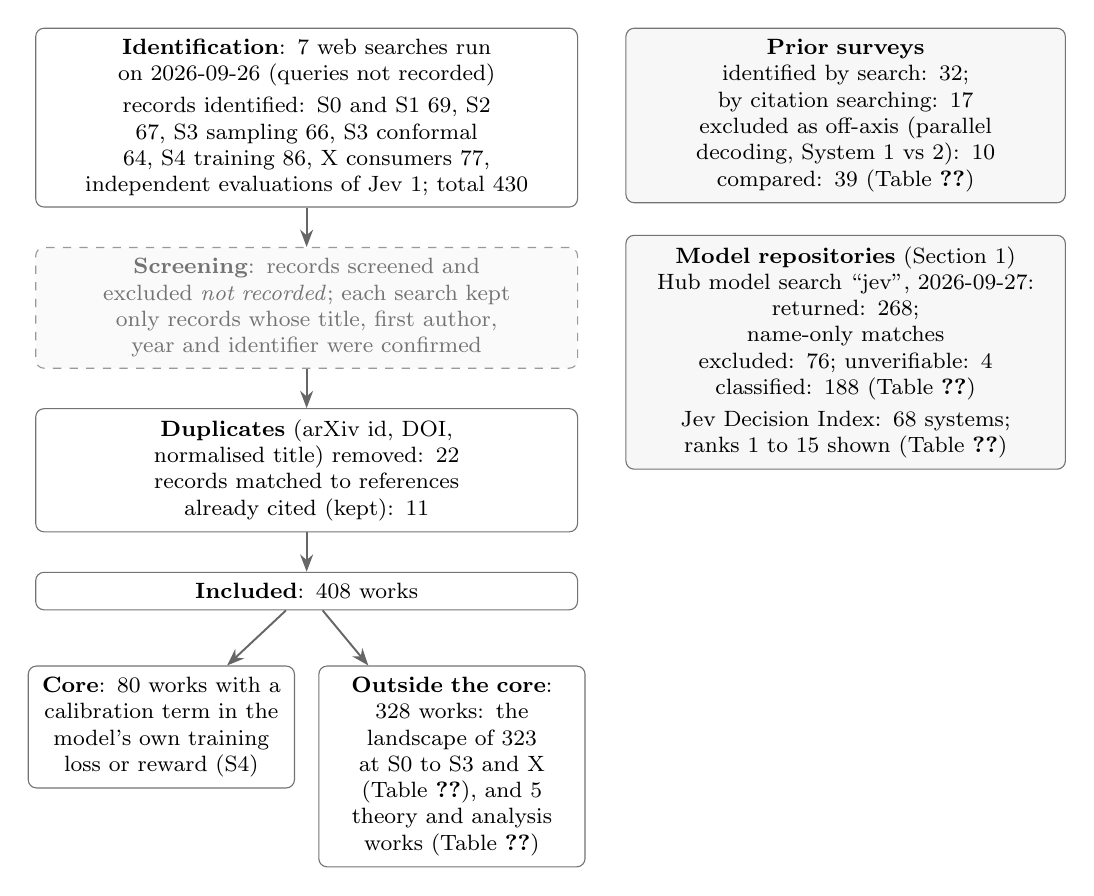
\begin{tikzpicture}[font=\footnotesize, box/.style={draw=black!55,rounded corners=3pt,align=center,text width=66mm,inner sep=4pt,fill=white},
  nl/.style={box,dashed,draw=black!40,text=black!55,fill=black!2}, side/.style={box,text width=53mm,fill=black!3},
  every node/.append style={execute at begin node={\hyphenpenalty=10000\exhyphenpenalty=10000}},
  ar/.style={-{Stealth[length=2.2mm]},black!60,line width=0.7pt}]
 \node[box] (id) {\textbf{Identification}: 7 web searches run on 2026-09-26 (queries not recorded)\\[2pt]
   records identified: S0 and S1 69, S2 67, S3 sampling 66, S3 conformal 64, S4 training 86, X consumers 77, independent evaluations of Jev 1; total 430};
 \node[nl, below=5mm of id]  (scr) {\textbf{Screening}: records screened and excluded \emph{not recorded}; each search kept only records whose title, first author, year and identifier were confirmed};
 \node[box, below=5mm of scr] (dup) {\textbf{Duplicates} (arXiv id, DOI, normalised title) removed: 22\\ records matched to references already cited (kept): 11};
 \node[box, below=5mm of dup] (inc) {\textbf{Included}: 408 works};
 \node[box, text width=31mm, below left=7mm and -33mm of inc] (core) {\textbf{Core}: 80 works with a calibration term in the model's own training loss or reward (S4)};
 \node[box, text width=31mm, below right=7mm and -33mm of inc] (bg) {\textbf{Outside the core}: 328 works: the landscape of 323 at S0 to S3 and X (Table~\ref{tab:landscape}), and 5 theory and analysis works (Table~\ref{tab:compare_s4})};
 \node[side, right=6mm of id.north east, anchor=north west] (sv) {\textbf{Prior surveys}\\ identified by search: 32; by citation searching: 17\\ excluded as off-axis (parallel decoding, System~1 vs~2): 10\\ compared: 39 (Table~\ref{tab:survey_compare})};
 \node[side, below=4mm of sv] (mr) {\textbf{Model repositories} (Section~1)\\ Hub model search ``jev'', 2026-09-27:\\ returned: 268;\\ name-only matches excluded: 76; unverifiable: 4\\ classified: 188 (Table~\ref{tab:jev_hf_ecosystem})\\[2pt] Jev Decision Index: 68 systems; ranks 1 to 15 shown (Table~\ref{tab:jev_decision_index})};
 \draw[ar] (id) -- (scr); \draw[ar] (scr) -- (dup); \draw[ar] (dup) -- (inc); \draw[ar] (inc) -- (core); \draw[ar] (inc) -- (bg);
\end{tikzpicture}
\caption{\textbf{Corpus construction flow}, laid out after PRISMA 2020. The main column counts the primary works; the side boxes
count the prior surveys and, for Tables~\ref{tab:jev_hf_ecosystem} and~\ref{tab:jev_decision_index}, the model repositories and the leaderboard. Screening counts were not recorded
and are marked rather than estimated. A work is core if and only if a calibration term enters the model's own training loss or
reward (Table~\ref{tab:definitions}); theory and analyses of such training are listed with the core in Table~\ref{tab:compare_s4}
but not counted in it.}
\Description{A top-to-bottom flow chart: identification from 7 web searches, a dashed screening box marked not recorded,
duplicate removal, inclusion, then a split into core training-stage works and landscape works. Two side boxes count the
prior surveys and the model repositories and leaderboard systems used in the appendix.}
\label{fig:prisma}
\end{figure}


\paragraph{Placement.} A work is in the corpus when its main contribution meets one of the stage
definitions of Table~\ref{tab:definitions}: it produces, maps, elicits, samples or trains the confidence
of a language model (S0 to S4), analyses how training changes calibration, or acts on a confidence or
fixes the output contract (X). Each work is placed by what its main contribution changes, not by the
task it is evaluated on, and each training-stage work was assigned to one family by reading it. A work is
\emph{core} if and only if a calibration term enters the model's own training loss or reward; the
\nTheory theory and analysis works are listed with the core but not counted in it, and the \nLandscape
works at the other stages form the landscape (Appendix~\ref{app:landscape}). The per-work fields of
Tables~\ref{tab:compare_s4} and~\ref{tab:landscape} (output contract, access, samples, guarantee,
trained, metric, task and action) were recorded for each paper. The fields were checked against the papers in
several review rounds and corrected where they disagreed, and a value that cannot be
determined from the paper is marked as such rather than guessed.

\paragraph{Prior surveys.} \nSurveysPhaseOne prior surveys were identified by search and the rest by
backward citation searching from the surveys found, \nSurveys in all. \nSurveysOffAxis of them, on parallel
and speculative decoding~\citep{xiao2023survey,li2025surveydiffusion,yu2025discrete,gwak2026accelerating,xia2024unlocking,hu2025speculative,ryu2024closer,zhou2024survey}
and on fast versus slow reasoning~\citep{li2025system,sui2025stop}, are off the axis of this survey
and are set aside; the remaining \nSurveysCompared are compared in Table~\ref{tab:survey_compare}. The
marks for reinforcement learning with a calibration reward were checked in the full text or the full
reference list of every survey.

\subsection{The corpus at a glance}
\label{sec:glance}

Figure~\ref{fig:corpus_overview} summarises the corpus and Figure~\ref{fig:corpus_dist} profiles it.
Extra inference (S3) is the largest stage, with \nSthree works, most of them conformal prediction sets,
risk control and sampling-based uncertainty; training (S4) follows with \nSfour, and the consumers of a
confidence (X) with \nX. Most
methods need the model's logits or weights (\nWhite white-box works against \nBlack that work from text
alone). Figure~\ref{fig:stage_trend} shows how recent the training stage is: \nCoreRecent of its
\nCore works appeared from 2024 to 2026 (\nCoreRecentPct), against \nBgRecent of the \nSzeroToSthree works at
the other stages over the same years (\nBgRecentPct).

% AUTO-GENERATED by build/gen_corpus.py from literature/corpus.tsv -- do not hand-edit.
\begin{figure}[t]
\centering
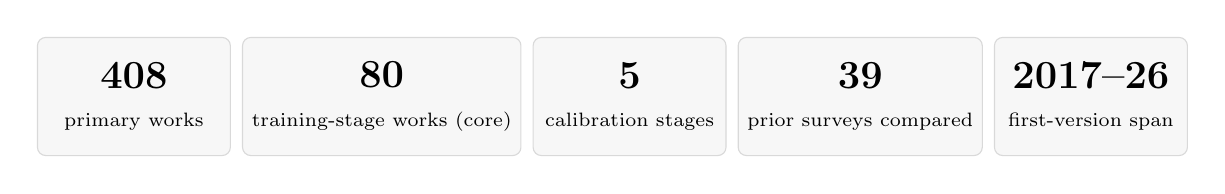
\begin{tikzpicture}
\matrix[column sep=4pt]{
\node[draw=black!15,fill=black!3,rounded corners=3pt,minimum width=2.45cm,minimum height=1.5cm,align=center] {\Large\bfseries 408\\[2pt]\scriptsize primary works}; & \node[draw=black!15,fill=black!3,rounded corners=3pt,minimum width=2.45cm,minimum height=1.5cm,align=center] {\Large\bfseries 80\\[2pt]\scriptsize training-stage works (core)}; & \node[draw=black!15,fill=black!3,rounded corners=3pt,minimum width=2.45cm,minimum height=1.5cm,align=center] {\Large\bfseries 5\\[2pt]\scriptsize calibration stages}; & \node[draw=black!15,fill=black!3,rounded corners=3pt,minimum width=2.45cm,minimum height=1.5cm,align=center] {\Large\bfseries 39\\[2pt]\scriptsize prior surveys compared}; & \node[draw=black!15,fill=black!3,rounded corners=3pt,minimum width=2.45cm,minimum height=1.5cm,align=center] {\Large\bfseries 2017--26\\[2pt]\scriptsize first-version span}; \\
};
\end{tikzpicture}\\[6pt]
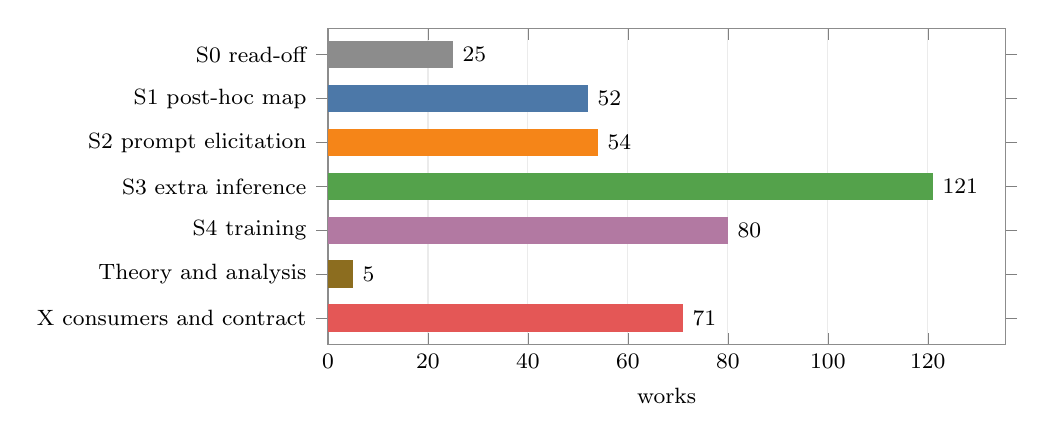
\begin{tikzpicture}
\begin{axis}[xbar,bar width=10pt,width=0.84\textwidth,height=5.6cm,xmin=0,
  symbolic y coords={{X consumers and contract},{Theory and analysis},{S4 training},{S3 extra inference},{S2 prompt elicitation},{S1 post-hoc map},{S0 read-off}},ytick={{X consumers and contract},{Theory and analysis},{S4 training},{S3 extra inference},{S2 prompt elicitation},{S1 post-hoc map},{S0 read-off}},y dir=normal,
  nodes near coords,nodes near coords style={font=\footnotesize},xlabel={\footnotesize works},tick label style={font=\footnotesize},
  axis line style={black!45},xmajorgrids,grid style={black!8},enlarge x limits={upper,value=0.12}]
\addplot[fill=stS0,draw=none,bar shift=0pt] coordinates {(25,{S0 read-off})};
\addplot[fill=stS1,draw=none,bar shift=0pt] coordinates {(52,{S1 post-hoc map})};
\addplot[fill=stS2,draw=none,bar shift=0pt] coordinates {(54,{S2 prompt elicitation})};
\addplot[fill=stS3,draw=none,bar shift=0pt] coordinates {(121,{S3 extra inference})};
\addplot[fill=stS4,draw=none,bar shift=0pt] coordinates {(80,{S4 training})};
\addplot[fill=stTH,draw=none,bar shift=0pt] coordinates {(5,{Theory and analysis})};
\addplot[fill=stX,draw=none,bar shift=0pt] coordinates {(71,{X consumers and contract})};
\end{axis}
\end{tikzpicture}
\caption{\textbf{The corpus at a glance.} 408 primary works (451 references cited across the figures and tables), placed by the stage at which
calibration enters (Table~\ref{tab:definitions}); the X group holds works that consume the confidence or fix the output
contract, and the theory group holds analyses of training-stage calibration. 39 prior surveys are compared in
Table~\ref{tab:survey_compare}.}
\Description{Five stat cards (works, training-stage works, stages, prior surveys and year span) above a horizontal bar
chart of works per stage.}
\label{fig:corpus_overview}
\end{figure}

% AUTO-GENERATED by build/gen_corpus.py from literature/corpus.tsv -- do not hand-edit.
\begin{figure}[t]
\centering
\definecolor{cc0}{HTML}{1F77B4}
\definecolor{cc1}{HTML}{FF7F0E}
\definecolor{cc2}{HTML}{2CA02C}
\definecolor{cc3}{HTML}{D62728}
\definecolor{cc4}{HTML}{9467BD}
\definecolor{cc5}{HTML}{8C564B}
\definecolor{cc6}{HTML}{E377C2}
\definecolor{cc7}{HTML}{17BECF}
\definecolor{cc8}{HTML}{BCBD22}
\definecolor{cc9}{HTML}{7F7F7F}
\begin{tikzpicture}
\begin{scope}\begin{axis}[ybar,bar width=9pt,width=0.5\textwidth,height=5cm,ymin=0,
  symbolic x coords={{2017},{2018},{2019},{2020},{2021},{2022},{2023},{2024},{2025},{2026*}},xtick={{2017},{2018},{2019},{2020},{2021},{2022},{2023},{2024},{2025},{2026*}},x tick label style={font=\scriptsize,rotate=45,anchor=east},
  nodes near coords,nodes near coords style={font=\scriptsize},title={\footnotesize\bfseries (a) Year of first version},
  ylabel={\scriptsize works},tick label style={font=\scriptsize},axis line style={black!45},tick pos=left,ymajorgrids,grid style={black!8},
  enlarge x limits=0.06,enlarge y limits={upper,value=0.18}]
\addplot[fill={rgb,255:red,158;green,202;blue,225},draw=none,bar shift=0pt] coordinates {({2017},1)};
\addplot[fill={rgb,255:red,143;green,188;blue,213},draw=none,bar shift=0pt] coordinates {({2018},2)};
\addplot[fill={rgb,255:red,129;green,174;blue,201},draw=none,bar shift=0pt] coordinates {({2019},3)};
\addplot[fill={rgb,255:red,115;green,160;blue,190},draw=none,bar shift=0pt] coordinates {({2020},9)};
\addplot[fill={rgb,255:red,101;green,146;blue,178},draw=none,bar shift=0pt] coordinates {({2021},12)};
\addplot[fill={rgb,255:red,87;green,133;blue,167},draw=none,bar shift=0pt] coordinates {({2022},18)};
\addplot[fill={rgb,255:red,73;green,119;blue,155},draw=none,bar shift=0pt] coordinates {({2023},66)};
\addplot[fill={rgb,255:red,59;green,105;blue,144},draw=none,bar shift=0pt] coordinates {({2024},138)};
\addplot[fill={rgb,255:red,45;green,91;blue,132},draw=none,bar shift=0pt] coordinates {({2025},97)};
\addplot[fill={rgb,255:red,31;green,78;blue,121},draw=none,bar shift=0pt] coordinates {({2026*},62)};
\end{axis}\end{scope}
\begin{scope}[xshift=0.5\textwidth]\begin{axis}[ybar,bar width=9pt,width=0.5\textwidth,height=5cm,ymin=0,
  symbolic x coords={{score},{free-text},{typed},{set},{constrained},{not determinable}},xtick={{score},{free-text},{typed},{set},{constrained},{not determinable}},x tick label style={font=\scriptsize,rotate=30,anchor=east},
  nodes near coords,nodes near coords style={font=\scriptsize},enlarge x limits=0.1,
  title={\footnotesize\bfseries (b) Output contract},ylabel={\scriptsize works},tick label style={font=\scriptsize},axis line style={black!45},tick pos=left,
  ymajorgrids,grid style={black!8},enlarge y limits={upper,value=0.18}]
\addplot[fill=cc0,draw=none,bar shift=0pt] coordinates {({score},147)};
\addplot[fill=cc1,draw=none,bar shift=0pt] coordinates {({free-text},119)};
\addplot[fill=cc2,draw=none,bar shift=0pt] coordinates {({typed},65)};
\addplot[fill=cc3,draw=none,bar shift=0pt] coordinates {({set},44)};
\addplot[fill=cc4,draw=none,bar shift=0pt] coordinates {({constrained},32)};
\addplot[fill=cc5,draw=none,bar shift=0pt] coordinates {({not determinable},1)};
\end{axis}\end{scope}
\begin{scope}[yshift=-6.2cm]\begin{axis}[ybar,bar width=9pt,width=0.5\textwidth,height=5cm,ymin=0,
  symbolic x coords={{QA},{generation},{reasoning},{classification},{other},{judging},{code},{robotics},{agentic}},xtick={{QA},{generation},{reasoning},{classification},{other},{judging},{code},{robotics},{agentic}},x tick label style={font=\scriptsize,rotate=30,anchor=east},
  nodes near coords,nodes near coords style={font=\scriptsize},enlarge x limits=0.1,
  title={\footnotesize\bfseries (c) Task},ylabel={\scriptsize works},tick label style={font=\scriptsize},axis line style={black!45},tick pos=left,
  ymajorgrids,grid style={black!8},enlarge y limits={upper,value=0.18}]
\addplot[fill=cc0,draw=none,bar shift=0pt] coordinates {({QA},178)};
\addplot[fill=cc1,draw=none,bar shift=0pt] coordinates {({generation},67)};
\addplot[fill=cc2,draw=none,bar shift=0pt] coordinates {({reasoning},56)};
\addplot[fill=cc3,draw=none,bar shift=0pt] coordinates {({classification},46)};
\addplot[fill=cc4,draw=none,bar shift=0pt] coordinates {({other},17)};
\addplot[fill=cc5,draw=none,bar shift=0pt] coordinates {({judging},16)};
\addplot[fill=cc6,draw=none,bar shift=0pt] coordinates {({code},14)};
\addplot[fill=cc7,draw=none,bar shift=0pt] coordinates {({robotics},8)};
\addplot[fill=cc8,draw=none,bar shift=0pt] coordinates {({agentic},6)};
\end{axis}\end{scope}
\begin{scope}[xshift=0.5\textwidth,yshift=-6.2cm]\begin{axis}[ybar,bar width=9pt,width=0.5\textwidth,height=5cm,ymin=0,
  symbolic x coords={{white},{black},{either},{not determinable}},xtick={{white},{black},{either},{not determinable}},x tick label style={font=\scriptsize,rotate=30,anchor=east},
  nodes near coords,nodes near coords style={font=\scriptsize},enlarge x limits=0.1,
  title={\footnotesize\bfseries (d) Access needed},ylabel={\scriptsize works},tick label style={font=\scriptsize},axis line style={black!45},tick pos=left,
  ymajorgrids,grid style={black!8},enlarge y limits={upper,value=0.18}]
\addplot[fill=cc0,draw=none,bar shift=0pt] coordinates {({white},221)};
\addplot[fill=cc1,draw=none,bar shift=0pt] coordinates {({black},126)};
\addplot[fill=cc2,draw=none,bar shift=0pt] coordinates {({either},50)};
\addplot[fill=cc3,draw=none,bar shift=0pt] coordinates {({not determinable},11)};
\end{axis}\end{scope}
\end{tikzpicture}
\caption{\textbf{Profile of the 408 corpus works} (Tables~\ref{tab:compare_s4} and~\ref{tab:landscape}). (a)~Year of first public version
(*2026 is partial); (b)~the output contract the confidence is attached to (the five contracts are defined in the caption of Table~\ref{tab:landscape}); (c)~task; (d)~the access a method needs:
white-box (logits or weights), black-box (text only) or either. ``not determinable'' marks a value that could not be determined from the paper.}
\Description{Four bar charts describing the corpus: works per year, per output contract, per task and per access level.}
\label{fig:corpus_dist}
\end{figure}

% AUTO-GENERATED by build/gen_corpus.py from literature/corpus.tsv -- do not hand-edit.
\begin{figure}[t]
\centering
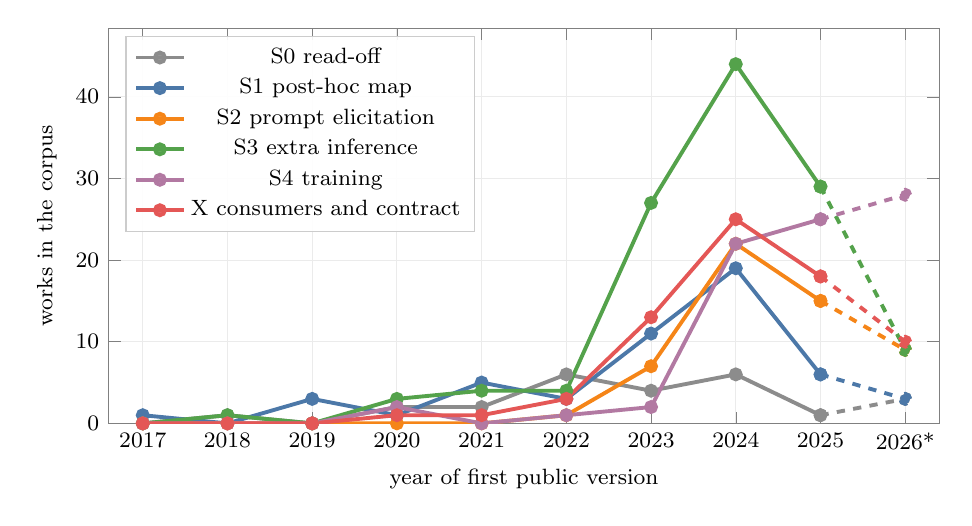
\begin{tikzpicture}
\begin{axis}[width=\textwidth,height=6.6cm,xmin=2016.6,xmax=2026.4,ymin=0,
  xtick={2017,2018,2019,2020,2021,2022,2023,2024,2025,2026},xticklabels={2017,2018,2019,2020,2021,2022,2023,2024,2025,2026*},
  ylabel={works in the corpus},xlabel={year of first public version},grid=major,grid style={black!8},
  legend style={at={(0.02,0.98)},anchor=north west,font=\footnotesize,draw=black!20,fill=white,fill opacity=0.9,text opacity=1},
  tick label style={font=\footnotesize},label style={font=\footnotesize},axis line style={black!50}]
\addplot[color=stS0,line width=1.4pt,mark=*,mark size=1.8pt] coordinates {(2017,0) (2018,1) (2019,0) (2020,2) (2021,2) (2022,6) (2023,4) (2024,6) (2025,1)}; \addlegendentry{S0 read-off}
\addplot[color=stS0,line width=1.4pt,dashed,mark=*,mark size=1.8pt,forget plot] coordinates {(2025,1) (2026,3)};
\addplot[color=stS1,line width=1.4pt,mark=*,mark size=1.8pt] coordinates {(2017,1) (2018,0) (2019,3) (2020,1) (2021,5) (2022,3) (2023,11) (2024,19) (2025,6)}; \addlegendentry{S1 post-hoc map}
\addplot[color=stS1,line width=1.4pt,dashed,mark=*,mark size=1.8pt,forget plot] coordinates {(2025,6) (2026,3)};
\addplot[color=stS2,line width=1.4pt,mark=*,mark size=1.8pt] coordinates {(2017,0) (2018,0) (2019,0) (2020,0) (2021,0) (2022,1) (2023,7) (2024,22) (2025,15)}; \addlegendentry{S2 prompt elicitation}
\addplot[color=stS2,line width=1.4pt,dashed,mark=*,mark size=1.8pt,forget plot] coordinates {(2025,15) (2026,9)};
\addplot[color=stS3,line width=1.4pt,mark=*,mark size=1.8pt] coordinates {(2017,0) (2018,1) (2019,0) (2020,3) (2021,4) (2022,4) (2023,27) (2024,44) (2025,29)}; \addlegendentry{S3 extra inference}
\addplot[color=stS3,line width=1.4pt,dashed,mark=*,mark size=1.8pt,forget plot] coordinates {(2025,29) (2026,9)};
\addplot[color=stS4,line width=1.4pt,mark=*,mark size=1.8pt] coordinates {(2017,0) (2018,0) (2019,0) (2020,2) (2021,0) (2022,1) (2023,2) (2024,22) (2025,25)}; \addlegendentry{S4 training}
\addplot[color=stS4,line width=1.4pt,dashed,mark=*,mark size=1.8pt,forget plot] coordinates {(2025,25) (2026,28)};
\addplot[color=stX,line width=1.4pt,mark=*,mark size=1.8pt] coordinates {(2017,0) (2018,0) (2019,0) (2020,1) (2021,1) (2022,3) (2023,13) (2024,25) (2025,18)}; \addlegendentry{X consumers and contract}
\addplot[color=stX,line width=1.4pt,dashed,mark=*,mark size=1.8pt,forget plot] coordinates {(2025,18) (2026,10)};
\end{axis}
\end{tikzpicture}
\caption{\textbf{Works per stage per year} (Tables~\ref{tab:compare_s4} and~\ref{tab:landscape}). 75 of the 80 training-stage (S4) works
appeared in 2024 to 2026 (94\%), against 166 of the 252 works at stages S0 to S3 (66\%) over the same years.
*2026 covers January to September, drawn dashed. The 5 theory and analysis works are not plotted.}
\Description{A line chart of corpus works per year from 2017 to 2026, one coloured line per stage. The
training-stage line rises steeply in the last three years; the last segment of each line is dashed because the final year is
partial.}
\label{fig:stage_trend}
\end{figure}


Figures~\ref{fig:method_gallery} and~\ref{fig:results_gallery} show, stage by stage, how the papers
themselves depict their methods and their results. Panels are chosen by a fixed rule and reproduced only
from papers whose licence permits reuse; the rule, and each panel's source figure, page and licence, are
in Table~\ref{tab:panel_provenance} (Appendix~\ref{app:provenance}).

% AUTO-GENERATED by build/gallery.py compile (pipeline tool gen_compilation_figure.py --fit)
% AUTO-GENERATED by tools/gen_compilation_figure.py -- vector TikZ, main-body, hyperlinked.
\begin{figure*}[tp]
\centering
\resizebox{\textwidth}{!}{%
\begin{tikzpicture}[x=1cm,y=1cm]
\definecolor{c355475}{HTML}{355475}
\definecolor{cAB5D10}{HTML}{AB5D10}
\definecolor{c3A7134}{HTML}{3A7134}
\definecolor{c7C5471}{HTML}{7C5471}
\definecolor{c9F3C3C}{HTML}{9F3C3C}
\fill[black!88] (0,0) rectangle (13.800,-0.580);
\node[anchor=west,text=white,font=\small\bfseries,inner sep=0] at (0.14,-0.290) {How confidence is produced and used, by stage};
\fill[c355475] (0,-0.580) rectangle (13.800,-1.080);
\node[anchor=west,text=white,font=\footnotesize\bfseries,inner sep=0] at (0.14,-0.830) {S1 post-hoc map};
\node[anchor=north west,inner sep=0] at (2.816,-1.150) {\href{https://arxiv.org/abs/2607.16799}{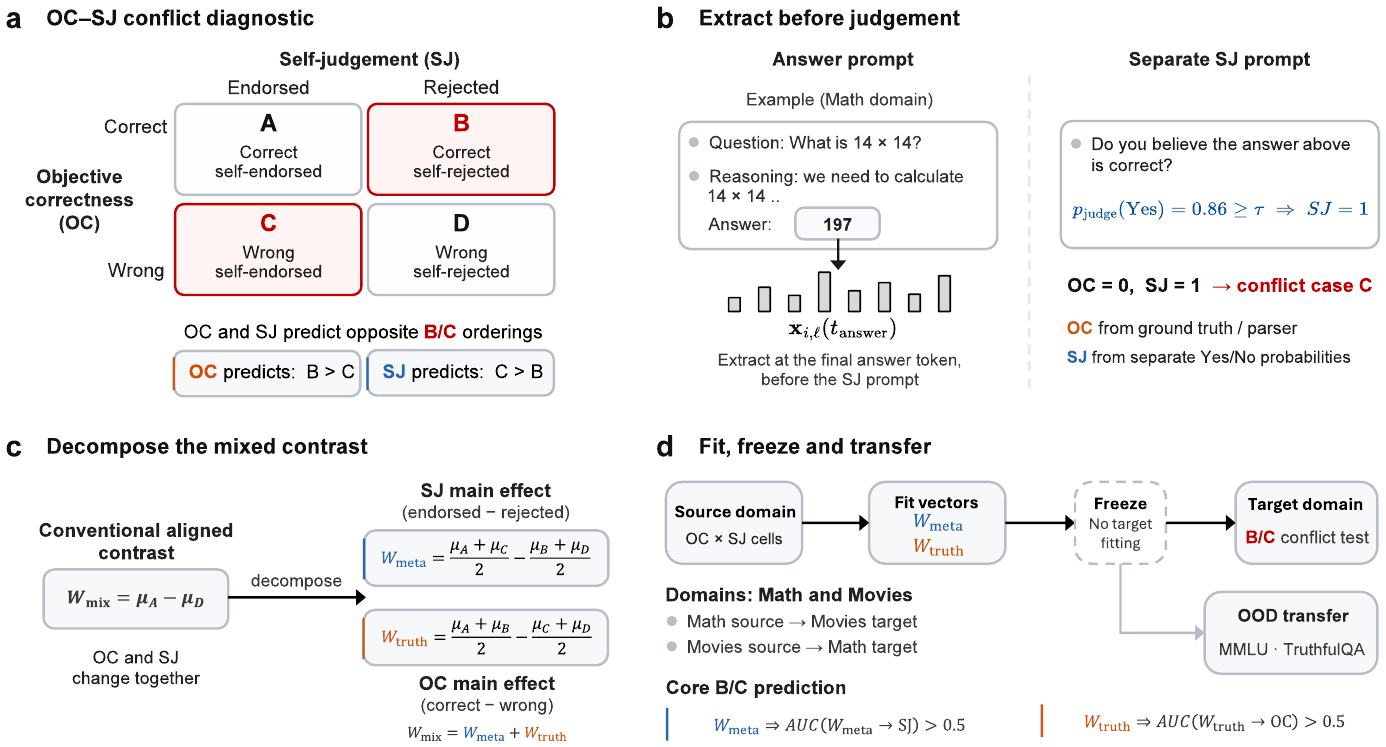
\includegraphics[width=2.676cm]{figures/img/method_gallery/tile_0.png}}};
\draw[black!35,line width=0.35pt] (2.816,-1.150) rectangle (5.492,-3.077);
\node[anchor=north west,text=ACMDarkBlue,font=\tiny\bfseries,inner sep=0] at (2.846,-3.107) {\href{https://arxiv.org/abs/2607.16799}{\adjustbox{max width=2.616cm}{Lu 2026}}};
\node[anchor=north west,text=black!60,font=\tiny,inner sep=0] at (2.846,-3.312) {\href{https://arxiv.org/abs/2607.16799}{Fig. 1, p.~2}};
\node[anchor=north west,inner sep=0] at (5.562,-1.150) {\href{https://arxiv.org/abs/2601.04277}{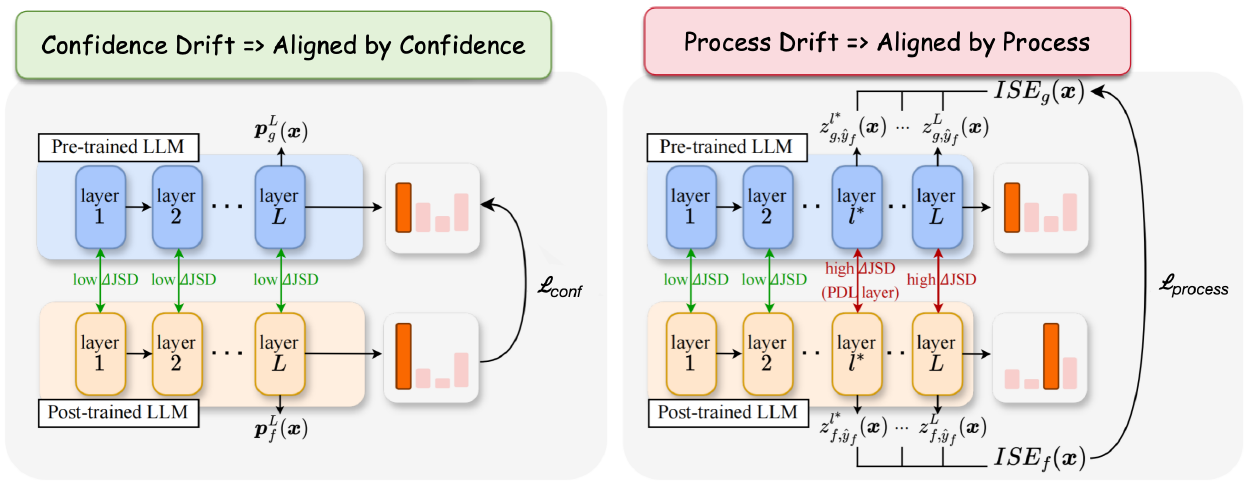
\includegraphics[width=2.676cm]{figures/img/method_gallery/tile_1.png}}};
\draw[black!35,line width=0.35pt] (5.562,-1.150) rectangle (8.238,-3.077);
\node[anchor=north west,text=ACMDarkBlue,font=\tiny\bfseries,inner sep=0] at (5.592,-3.107) {\href{https://arxiv.org/abs/2601.04277}{\adjustbox{max width=2.616cm}{Luo et al. 2026}}};
\node[anchor=north west,text=black!60,font=\tiny,inner sep=0] at (5.592,-3.312) {\href{https://arxiv.org/abs/2601.04277}{Fig. 1, p.~2}};
\node[anchor=north west,inner sep=0] at (8.308,-1.150) {\href{https://arxiv.org/abs/2505.23783}{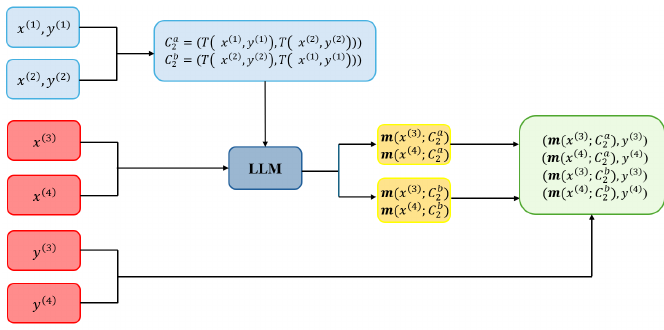
\includegraphics[width=2.676cm]{figures/img/method_gallery/tile_2.png}}};
\draw[black!35,line width=0.35pt] (8.308,-1.150) rectangle (10.984,-3.077);
\node[anchor=north west,text=ACMDarkBlue,font=\tiny\bfseries,inner sep=0] at (8.338,-3.107) {\href{https://arxiv.org/abs/2505.23783}{\adjustbox{max width=2.616cm}{Gundem et al. 2025}}};
\node[anchor=north west,text=black!60,font=\tiny,inner sep=0] at (8.338,-3.312) {\href{https://arxiv.org/abs/2505.23783}{Fig. 2, p.~5}};
\fill[cAB5D10] (0,-3.567) rectangle (13.800,-4.067);
\node[anchor=west,text=white,font=\footnotesize\bfseries,inner sep=0] at (0.14,-3.817) {S2 prompt elicitation};
\node[anchor=north west,inner sep=0] at (4.189,-4.137) {\href{https://arxiv.org/abs/2606.17234}{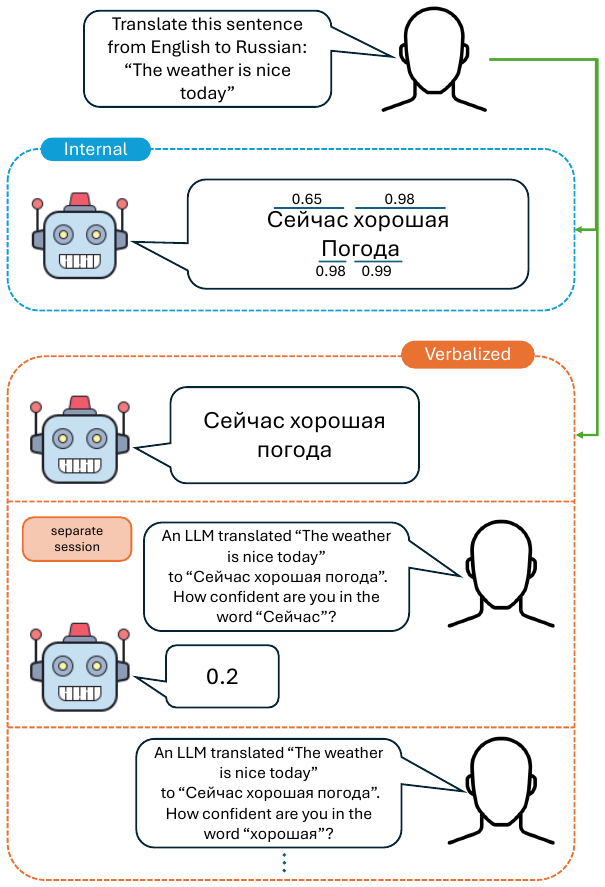
\includegraphics[width=2.676cm]{figures/img/method_gallery/tile_3.png}}};
\draw[black!35,line width=0.35pt] (4.189,-4.137) rectangle (6.865,-6.063);
\node[anchor=north west,text=ACMDarkBlue,font=\tiny\bfseries,inner sep=0] at (4.219,-6.093) {\href{https://arxiv.org/abs/2606.17234}{\adjustbox{max width=2.616cm}{Marashian et al. 2026}}};
\node[anchor=north west,text=black!60,font=\tiny,inner sep=0] at (4.219,-6.298) {\href{https://arxiv.org/abs/2606.17234}{Fig. 1, p.~1}};
\node[anchor=north west,inner sep=0] at (6.935,-4.137) {\href{https://arxiv.org/abs/2405.16282}{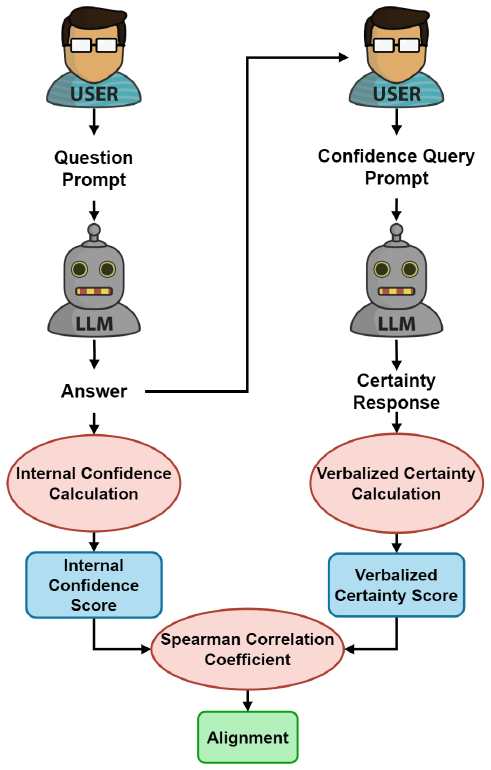
\includegraphics[width=2.676cm]{figures/img/method_gallery/tile_4.png}}};
\draw[black!35,line width=0.35pt] (6.935,-4.137) rectangle (9.611,-6.063);
\node[anchor=north west,text=ACMDarkBlue,font=\tiny\bfseries,inner sep=0] at (6.965,-6.093) {\href{https://arxiv.org/abs/2405.16282}{\adjustbox{max width=2.616cm}{Kumar et al. 2024}}};
\node[anchor=north west,text=black!60,font=\tiny,inner sep=0] at (6.965,-6.298) {\href{https://arxiv.org/abs/2405.16282}{Fig. 1, p.~1}};
\fill[c3A7134] (0,-6.553) rectangle (13.800,-7.053);
\node[anchor=west,text=white,font=\footnotesize\bfseries,inner sep=0] at (0.14,-6.803) {S3 extra inference};
\node[anchor=north west,inner sep=0] at (2.816,-7.123) {\href{https://arxiv.org/abs/2505.09427}{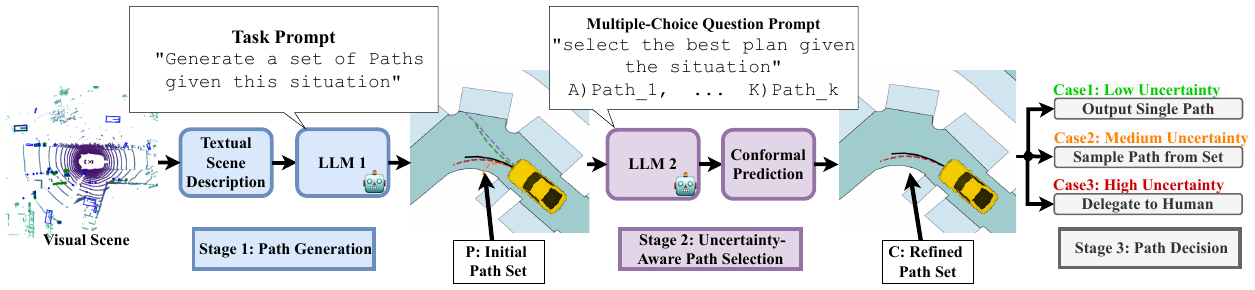
\includegraphics[width=2.676cm]{figures/img/method_gallery/tile_5.png}}};
\draw[black!35,line width=0.35pt] (2.816,-7.123) rectangle (5.492,-9.050);
\node[anchor=north west,text=ACMDarkBlue,font=\tiny\bfseries,inner sep=0] at (2.846,-9.080) {\href{https://arxiv.org/abs/2505.09427}{\adjustbox{max width=2.616cm}{Doula et al. 2025}}};
\node[anchor=north west,text=black!60,font=\tiny,inner sep=0] at (2.846,-9.285) {\href{https://arxiv.org/abs/2505.09427}{Fig. 1, p.~3}};
\node[anchor=north west,inner sep=0] at (5.562,-7.123) {\href{https://arxiv.org/abs/2305.13281}{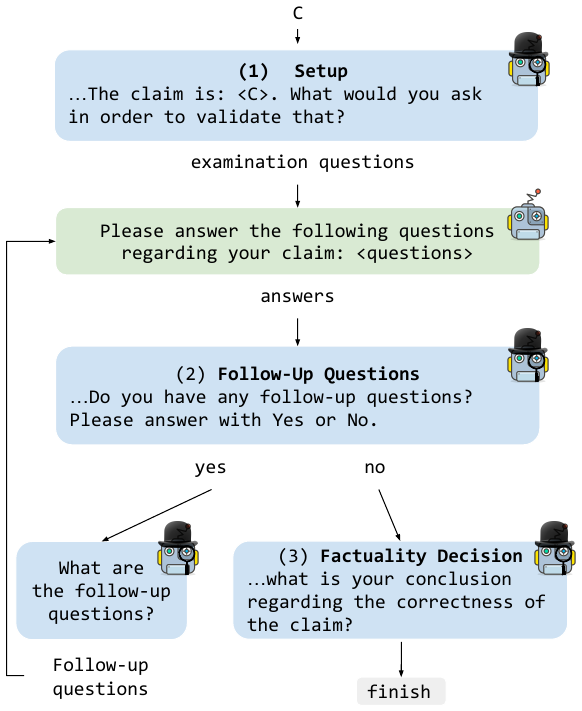
\includegraphics[width=2.676cm]{figures/img/method_gallery/tile_6.png}}};
\draw[black!35,line width=0.35pt] (5.562,-7.123) rectangle (8.238,-9.050);
\node[anchor=north west,text=ACMDarkBlue,font=\tiny\bfseries,inner sep=0] at (5.592,-9.080) {\href{https://arxiv.org/abs/2305.13281}{\adjustbox{max width=2.616cm}{Cohen et al. 2023}}};
\node[anchor=north west,text=black!60,font=\tiny,inner sep=0] at (5.592,-9.285) {\href{https://arxiv.org/abs/2305.13281}{Fig. 2, p.~3}};
\node[anchor=north west,inner sep=0] at (8.308,-7.123) {\href{https://arxiv.org/abs/2502.20285}{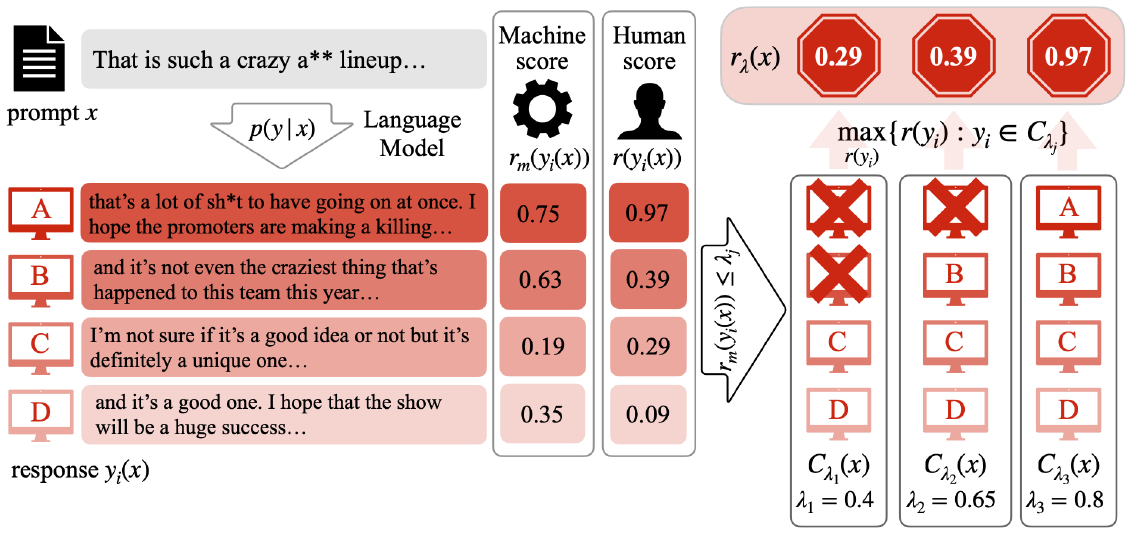
\includegraphics[width=2.676cm]{figures/img/method_gallery/tile_7.png}}};
\draw[black!35,line width=0.35pt] (8.308,-7.123) rectangle (10.984,-9.050);
\node[anchor=north west,text=ACMDarkBlue,font=\tiny\bfseries,inner sep=0] at (8.338,-9.080) {\href{https://arxiv.org/abs/2502.20285}{\adjustbox{max width=2.616cm}{Chen et al. 2025b}}};
\node[anchor=north west,text=black!60,font=\tiny,inner sep=0] at (8.338,-9.285) {\href{https://arxiv.org/abs/2502.20285}{Fig. 3, p.~8}};
\fill[c7C5471] (0,-9.540) rectangle (13.800,-10.040);
\node[anchor=west,text=white,font=\footnotesize\bfseries,inner sep=0] at (0.14,-9.790) {S4 training};
\node[anchor=north west,inner sep=0] at (2.816,-10.110) {\href{https://arxiv.org/abs/2607.01612}{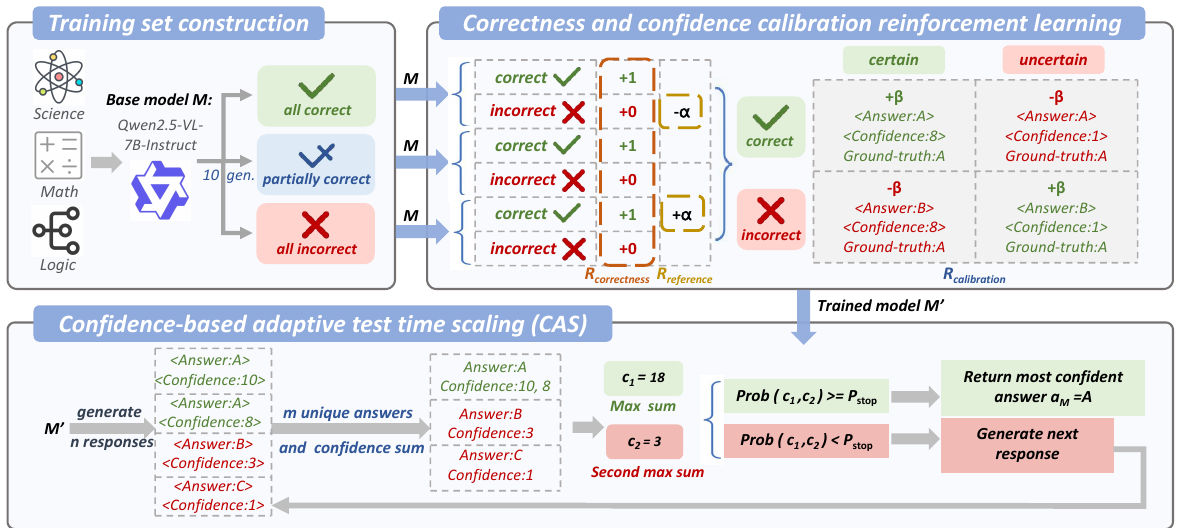
\includegraphics[width=2.676cm]{figures/img/method_gallery/tile_8.png}}};
\draw[black!35,line width=0.35pt] (2.816,-10.110) rectangle (5.492,-12.037);
\node[anchor=north west,text=ACMDarkBlue,font=\tiny\bfseries,inner sep=0] at (2.846,-12.067) {\href{https://arxiv.org/abs/2607.01612}{\adjustbox{max width=2.616cm}{Yang et al. 2026b}}};
\node[anchor=north west,text=black!60,font=\tiny,inner sep=0] at (2.846,-12.272) {\href{https://arxiv.org/abs/2607.01612}{Fig. 1, p.~3}};
\node[anchor=north west,inner sep=0] at (5.562,-10.110) {\href{https://arxiv.org/abs/2604.05306}{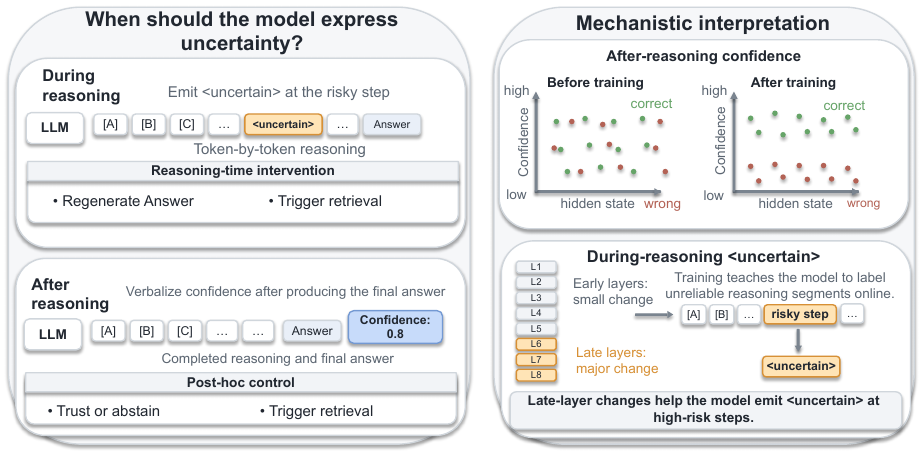
\includegraphics[width=2.676cm]{figures/img/method_gallery/tile_9.png}}};
\draw[black!35,line width=0.35pt] (5.562,-10.110) rectangle (8.238,-12.037);
\node[anchor=north west,text=ACMDarkBlue,font=\tiny\bfseries,inner sep=0] at (5.592,-12.067) {\href{https://arxiv.org/abs/2604.05306}{\adjustbox{max width=2.616cm}{Guo et al. 2026}}};
\node[anchor=north west,text=black!60,font=\tiny,inner sep=0] at (5.592,-12.272) {\href{https://arxiv.org/abs/2604.05306}{Fig. 1, p.~2}};
\node[anchor=north west,inner sep=0] at (8.308,-10.110) {\href{https://arxiv.org/abs/2604.22779}{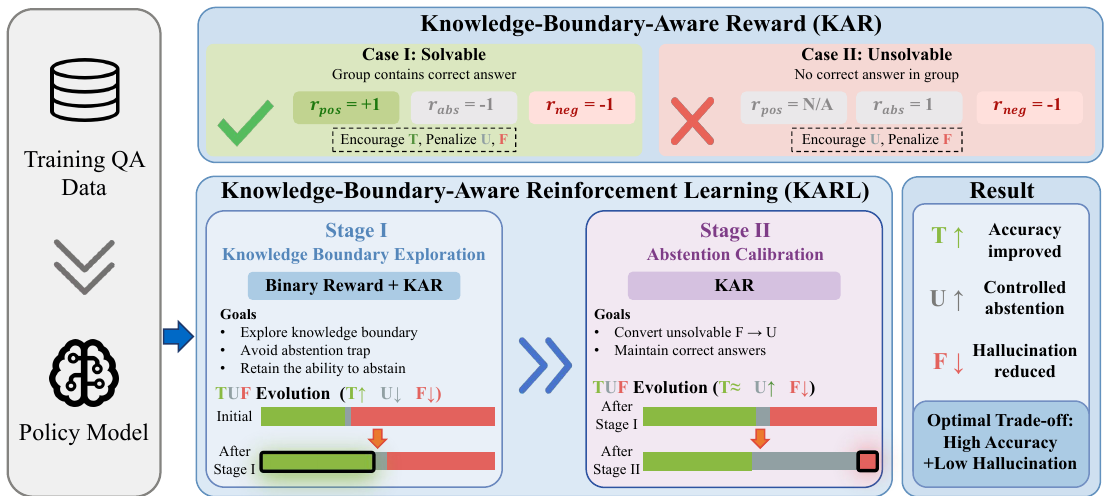
\includegraphics[width=2.676cm]{figures/img/method_gallery/tile_10.png}}};
\draw[black!35,line width=0.35pt] (8.308,-10.110) rectangle (10.984,-12.037);
\node[anchor=north west,text=ACMDarkBlue,font=\tiny\bfseries,inner sep=0] at (8.338,-12.067) {\href{https://arxiv.org/abs/2604.22779}{\adjustbox{max width=2.616cm}{Gao et al. 2026}}};
\node[anchor=north west,text=black!60,font=\tiny,inner sep=0] at (8.338,-12.272) {\href{https://arxiv.org/abs/2604.22779}{Fig. 4, p.~4}};
\fill[c9F3C3C] (0,-12.527) rectangle (13.800,-13.027);
\node[anchor=west,text=white,font=\footnotesize\bfseries,inner sep=0] at (0.14,-12.777) {X consumers and contract};
\node[anchor=north west,inner sep=0] at (2.816,-13.097) {\href{https://arxiv.org/abs/2505.04016}{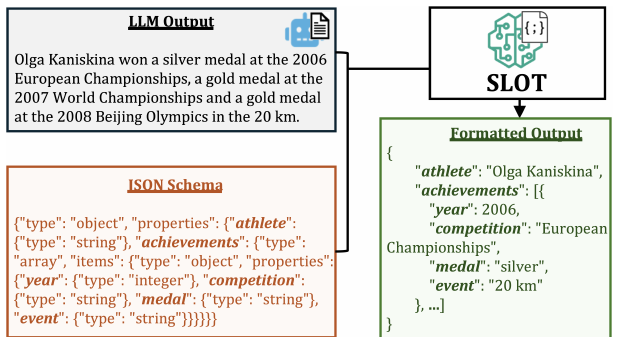
\includegraphics[width=2.676cm]{figures/img/method_gallery/tile_11.png}}};
\draw[black!35,line width=0.35pt] (2.816,-13.097) rectangle (5.492,-15.024);
\node[anchor=north west,text=ACMDarkBlue,font=\tiny\bfseries,inner sep=0] at (2.846,-15.054) {\href{https://arxiv.org/abs/2505.04016}{\adjustbox{max width=2.616cm}{Wang et al. 2025e}}};
\node[anchor=north west,text=black!60,font=\tiny,inner sep=0] at (2.846,-15.259) {\href{https://arxiv.org/abs/2505.04016}{Fig. 1, p.~1}};
\node[anchor=north west,inner sep=0] at (5.562,-13.097) {\href{https://arxiv.org/abs/2509.21837}{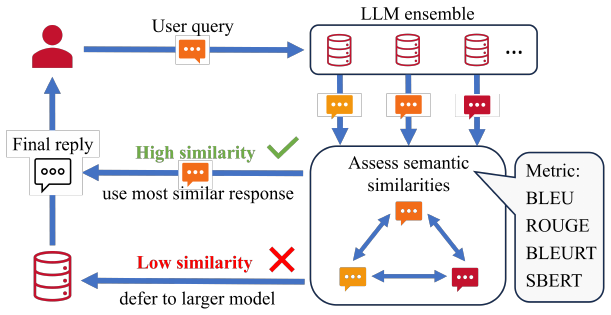
\includegraphics[width=2.676cm]{figures/img/method_gallery/tile_12.png}}};
\draw[black!35,line width=0.35pt] (5.562,-13.097) rectangle (8.238,-15.024);
\node[anchor=north west,text=ACMDarkBlue,font=\tiny\bfseries,inner sep=0] at (5.592,-15.054) {\href{https://arxiv.org/abs/2509.21837}{\adjustbox{max width=2.616cm}{Soiffer et al. 2025}}};
\node[anchor=north west,text=black!60,font=\tiny,inner sep=0] at (5.592,-15.259) {\href{https://arxiv.org/abs/2509.21837}{Fig. 1, p.~1}};
\node[anchor=north west,inner sep=0] at (8.308,-13.097) {\href{https://arxiv.org/abs/2305.11860}{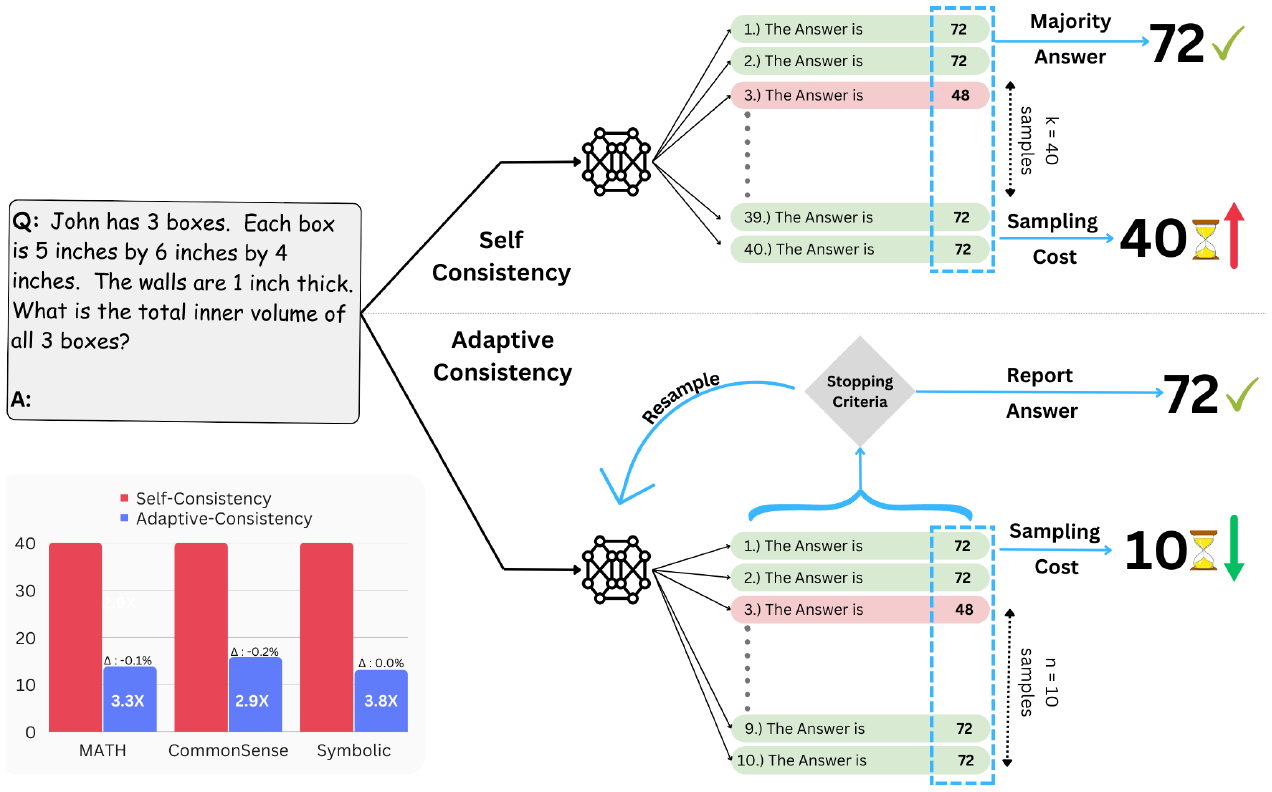
\includegraphics[width=2.676cm]{figures/img/method_gallery/tile_13.png}}};
\draw[black!35,line width=0.35pt] (8.308,-13.097) rectangle (10.984,-15.024);
\node[anchor=north west,text=ACMDarkBlue,font=\tiny\bfseries,inner sep=0] at (8.338,-15.054) {\href{https://arxiv.org/abs/2305.11860}{\adjustbox{max width=2.616cm}{Aggarwal et al. 2023}}};
\node[anchor=north west,text=black!60,font=\tiny,inner sep=0] at (8.338,-15.259) {\href{https://arxiv.org/abs/2305.11860}{Fig. 1, p.~2}};
\end{tikzpicture}}
\caption{\textbf{How confidence is produced and used, by stage.} Each panel shows a whole figure of the cited paper, reproduced under its CC BY licence; its label links to the paper. The selection rule and each panel's figure, page and licence are in Table~\ref{tab:panel_provenance}. S0 read-off has no panel: no reusable figure passed the check (Table~\ref{tab:panel_provenance}).}
\Description{A labelled grid of images, each a hyperlink annotated with its system name and source figure number.}
\label{fig:method_gallery}
\end{figure*}

% AUTO-GENERATED by build/gallery.py compile (pipeline tool gen_compilation_figure.py --fit)
% AUTO-GENERATED by tools/gen_compilation_figure.py -- vector TikZ, main-body, hyperlinked.
\begin{figure*}[tp]
\centering
\resizebox{\textwidth}{!}{%
\begin{tikzpicture}[x=1cm,y=1cm]
\definecolor{c626262}{HTML}{626262}
\definecolor{c355475}{HTML}{355475}
\definecolor{cAB5D10}{HTML}{AB5D10}
\definecolor{c3A7134}{HTML}{3A7134}
\definecolor{c7C5471}{HTML}{7C5471}
\definecolor{c9F3C3C}{HTML}{9F3C3C}
\fill[black!88] (0,0) rectangle (13.800,-0.580);
\node[anchor=west,text=white,font=\small\bfseries,inner sep=0] at (0.14,-0.290) {What calibration looks like in results, by stage};
\fill[c626262] (0,-0.580) rectangle (13.800,-1.080);
\node[anchor=west,text=white,font=\footnotesize\bfseries,inner sep=0] at (0.14,-0.830) {S0 read-off};
\node[anchor=north west,inner sep=0] at (4.189,-1.150) {\href{https://arxiv.org/abs/2211.07443}{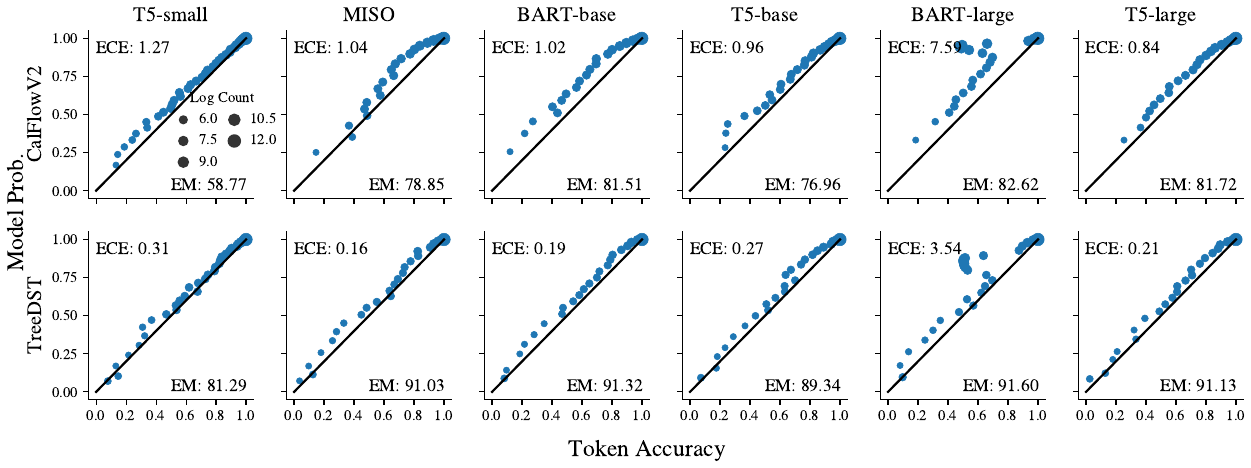
\includegraphics[width=2.676cm]{figures/img/results_gallery/tile_0.png}}};
\draw[black!35,line width=0.35pt] (4.189,-1.150) rectangle (6.865,-3.077);
\node[anchor=north west,text=ACMDarkBlue,font=\tiny\bfseries,inner sep=0] at (4.219,-3.107) {\href{https://arxiv.org/abs/2211.07443}{\adjustbox{max width=2.616cm}{Stengel-Eskin and Van Durme 2023}}};
\node[anchor=north west,text=black!60,font=\tiny,inner sep=0] at (4.219,-3.312) {\href{https://arxiv.org/abs/2211.07443}{Fig. 1, p.~6}};
\node[anchor=north west,inner sep=0] at (6.935,-1.150) {\href{https://arxiv.org/abs/2606.03437}{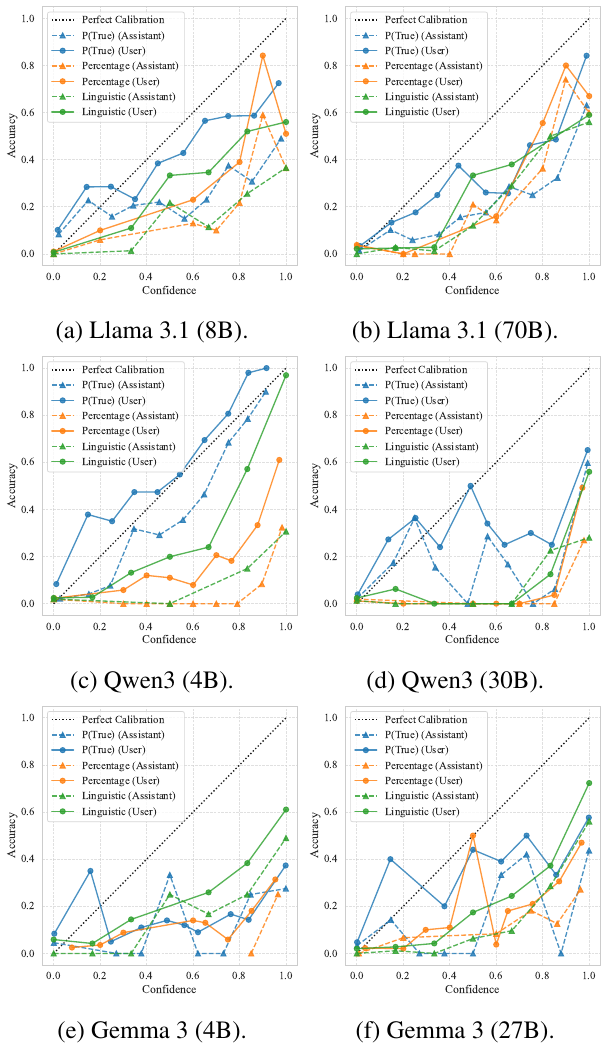
\includegraphics[width=2.676cm]{figures/img/results_gallery/tile_1.png}}};
\draw[black!35,line width=0.35pt] (6.935,-1.150) rectangle (9.611,-3.077);
\node[anchor=north west,text=ACMDarkBlue,font=\tiny\bfseries,inner sep=0] at (6.965,-3.107) {\href{https://arxiv.org/abs/2606.03437}{\adjustbox{max width=2.616cm}{Sanz-Guerrero et al. 2026}}};
\node[anchor=north west,text=black!60,font=\tiny,inner sep=0] at (6.965,-3.312) {\href{https://arxiv.org/abs/2606.03437}{Fig. 4, p.~6}};
\fill[c355475] (0,-3.567) rectangle (13.800,-4.067);
\node[anchor=west,text=white,font=\footnotesize\bfseries,inner sep=0] at (0.14,-3.817) {S1 post-hoc map};
\node[anchor=north west,inner sep=0] at (2.816,-4.137) {\href{https://arxiv.org/abs/2312.03729}{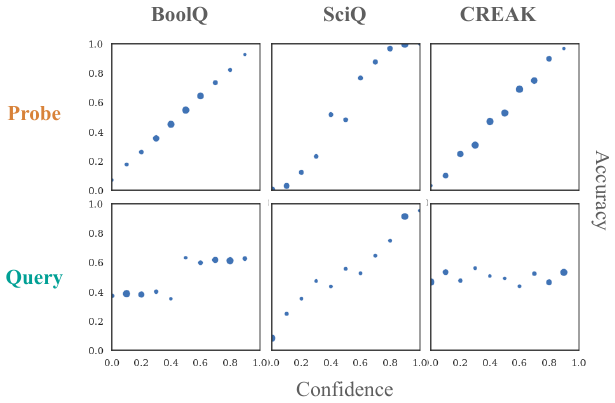
\includegraphics[width=2.676cm]{figures/img/results_gallery/tile_2.png}}};
\draw[black!35,line width=0.35pt] (2.816,-4.137) rectangle (5.492,-6.063);
\node[anchor=north west,text=ACMDarkBlue,font=\tiny\bfseries,inner sep=0] at (2.846,-6.093) {\href{https://arxiv.org/abs/2312.03729}{\adjustbox{max width=2.616cm}{Liu et al. 2023a}}};
\node[anchor=north west,text=black!60,font=\tiny,inner sep=0] at (2.846,-6.298) {\href{https://arxiv.org/abs/2312.03729}{Fig. 2, p.~3}};
\node[anchor=north west,inner sep=0] at (5.562,-4.137) {\href{https://arxiv.org/abs/2601.04277}{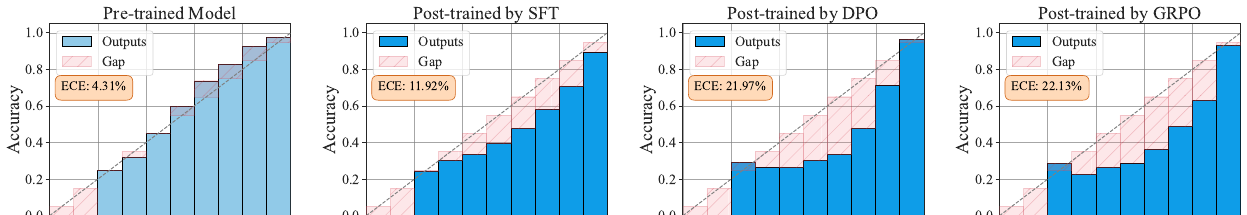
\includegraphics[width=2.676cm]{figures/img/results_gallery/tile_3.png}}};
\draw[black!35,line width=0.35pt] (5.562,-4.137) rectangle (8.238,-6.063);
\node[anchor=north west,text=ACMDarkBlue,font=\tiny\bfseries,inner sep=0] at (5.592,-6.093) {\href{https://arxiv.org/abs/2601.04277}{\adjustbox{max width=2.616cm}{Luo et al. 2026}}};
\node[anchor=north west,text=black!60,font=\tiny,inner sep=0] at (5.592,-6.298) {\href{https://arxiv.org/abs/2601.04277}{Fig. 5, p.~15}};
\node[anchor=north west,inner sep=0] at (8.308,-4.137) {\href{https://arxiv.org/abs/2505.16690}{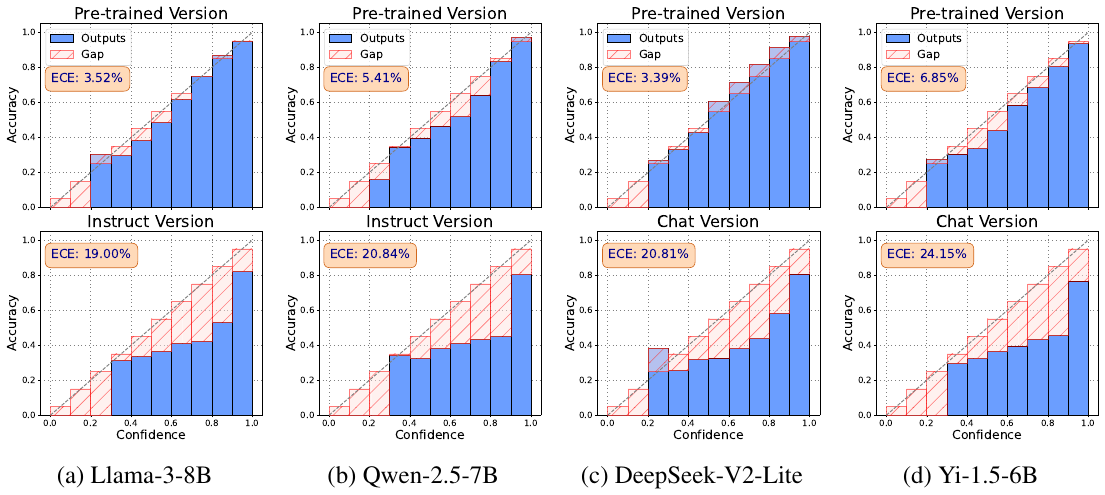
\includegraphics[width=2.676cm]{figures/img/results_gallery/tile_4.png}}};
\draw[black!35,line width=0.35pt] (8.308,-4.137) rectangle (10.984,-6.063);
\node[anchor=north west,text=ACMDarkBlue,font=\tiny\bfseries,inner sep=0] at (8.338,-6.093) {\href{https://arxiv.org/abs/2505.16690}{\adjustbox{max width=2.616cm}{Luo et al. 2025}}};
\node[anchor=north west,text=black!60,font=\tiny,inner sep=0] at (8.338,-6.298) {\href{https://arxiv.org/abs/2505.16690}{Fig. 1, p.~3}};
\fill[cAB5D10] (0,-6.553) rectangle (13.800,-7.053);
\node[anchor=west,text=white,font=\footnotesize\bfseries,inner sep=0] at (0.14,-6.803) {S2 prompt elicitation};
\node[anchor=north west,inner sep=0] at (2.816,-7.123) {\href{https://arxiv.org/abs/2606.17234}{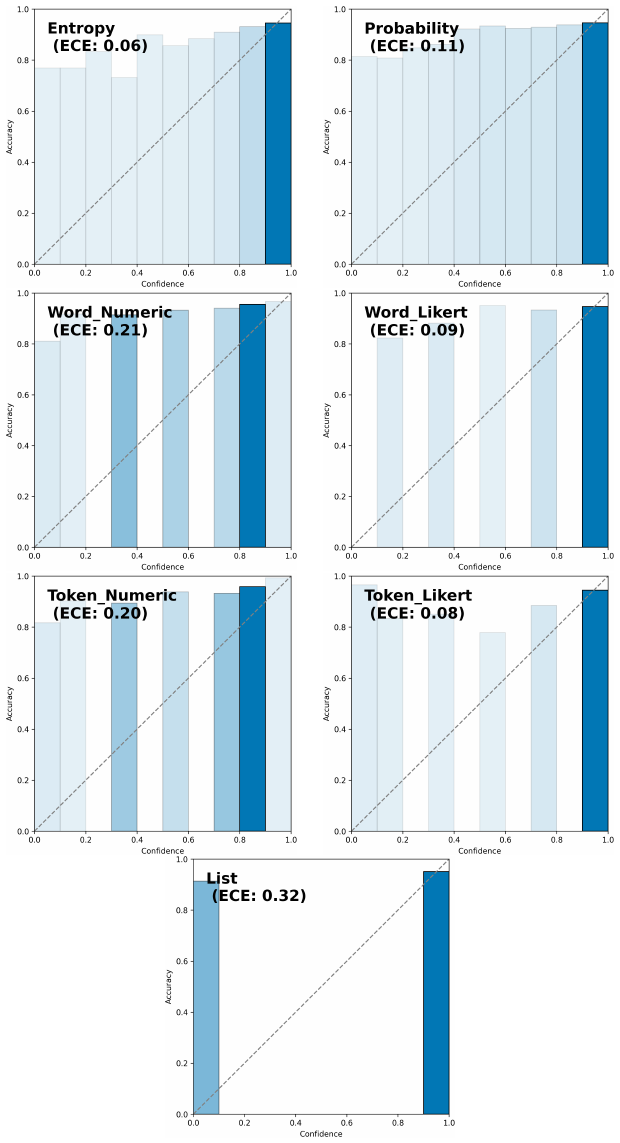
\includegraphics[width=2.676cm]{figures/img/results_gallery/tile_5.png}}};
\draw[black!35,line width=0.35pt] (2.816,-7.123) rectangle (5.492,-9.050);
\node[anchor=north west,text=ACMDarkBlue,font=\tiny\bfseries,inner sep=0] at (2.846,-9.080) {\href{https://arxiv.org/abs/2606.17234}{\adjustbox{max width=2.616cm}{Marashian et al. 2026}}};
\node[anchor=north west,text=black!60,font=\tiny,inner sep=0] at (2.846,-9.285) {\href{https://arxiv.org/abs/2606.17234}{Fig. 2, p.~5}};
\node[anchor=north west,inner sep=0] at (5.562,-7.123) {\href{https://arxiv.org/abs/2404.09127}{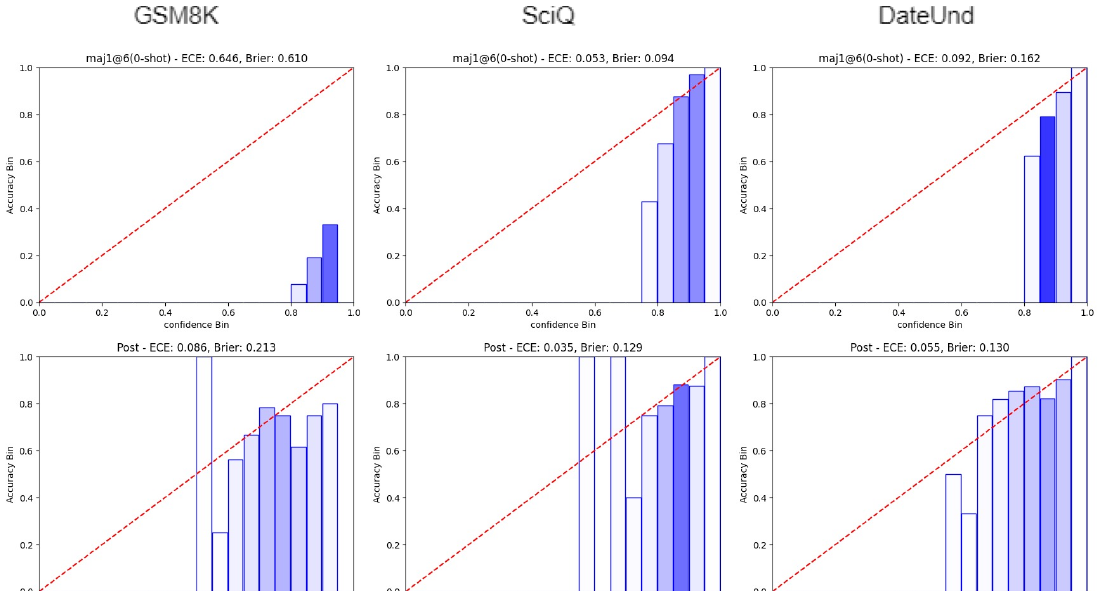
\includegraphics[width=2.676cm]{figures/img/results_gallery/tile_6.png}}};
\draw[black!35,line width=0.35pt] (5.562,-7.123) rectangle (8.238,-9.050);
\node[anchor=north west,text=ACMDarkBlue,font=\tiny\bfseries,inner sep=0] at (5.592,-9.080) {\href{https://arxiv.org/abs/2404.09127}{\adjustbox{max width=2.616cm}{Yang et al. 2024c}}};
\node[anchor=north west,text=black!60,font=\tiny,inner sep=0] at (5.592,-9.285) {\href{https://arxiv.org/abs/2404.09127}{Fig. 3, p.~11}};
\node[anchor=north west,inner sep=0] at (8.308,-7.123) {\href{https://arxiv.org/abs/2603.29559}{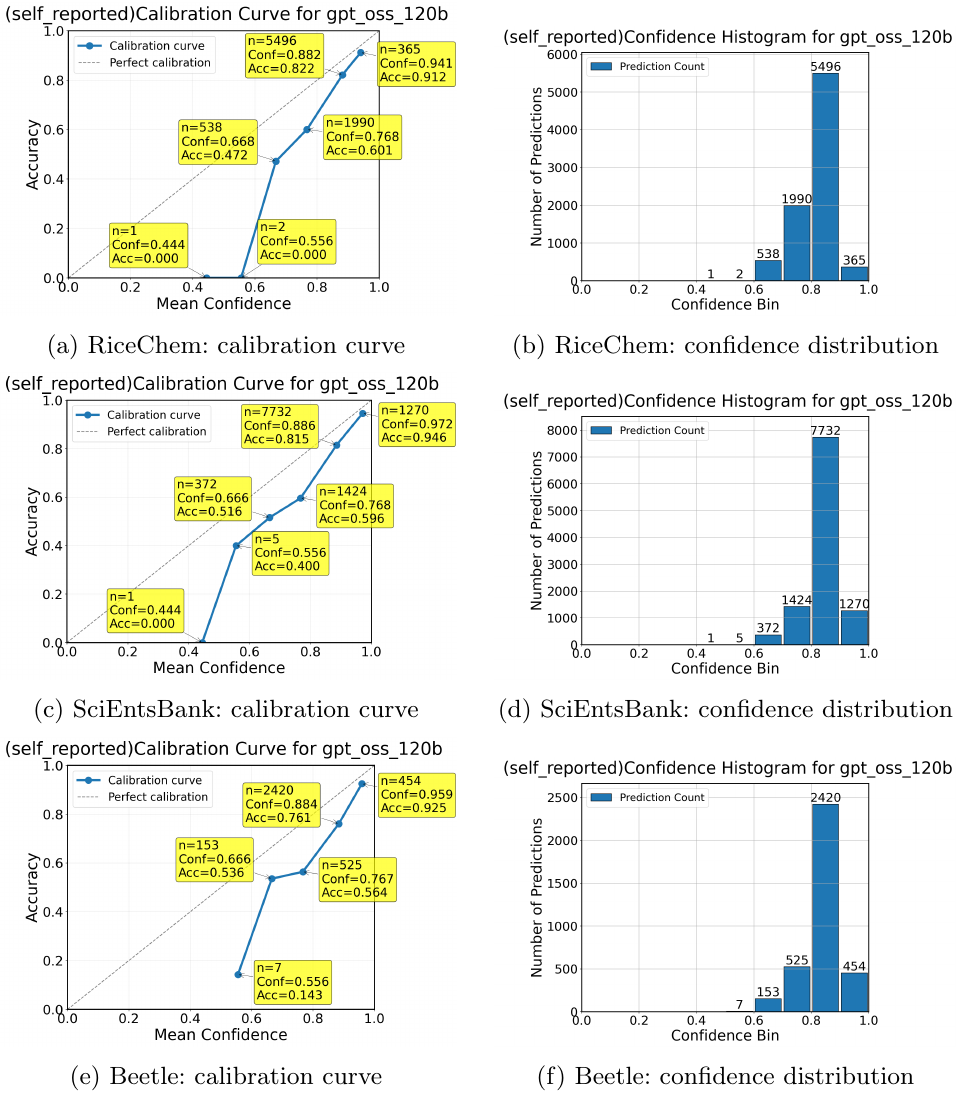
\includegraphics[width=2.676cm]{figures/img/results_gallery/tile_7.png}}};
\draw[black!35,line width=0.35pt] (8.308,-7.123) rectangle (10.984,-9.050);
\node[anchor=north west,text=ACMDarkBlue,font=\tiny\bfseries,inner sep=0] at (8.338,-9.080) {\href{https://arxiv.org/abs/2603.29559}{\adjustbox{max width=2.616cm}{Ferrer et al. 2026}}};
\node[anchor=north west,text=black!60,font=\tiny,inner sep=0] at (8.338,-9.285) {\href{https://arxiv.org/abs/2603.29559}{Fig. 1, p.~10}};
\fill[c3A7134] (0,-9.540) rectangle (13.800,-10.040);
\node[anchor=west,text=white,font=\footnotesize\bfseries,inner sep=0] at (0.14,-9.790) {S3 extra inference};
\node[anchor=north west,inner sep=0] at (2.816,-10.110) {\href{https://arxiv.org/abs/2402.00707}{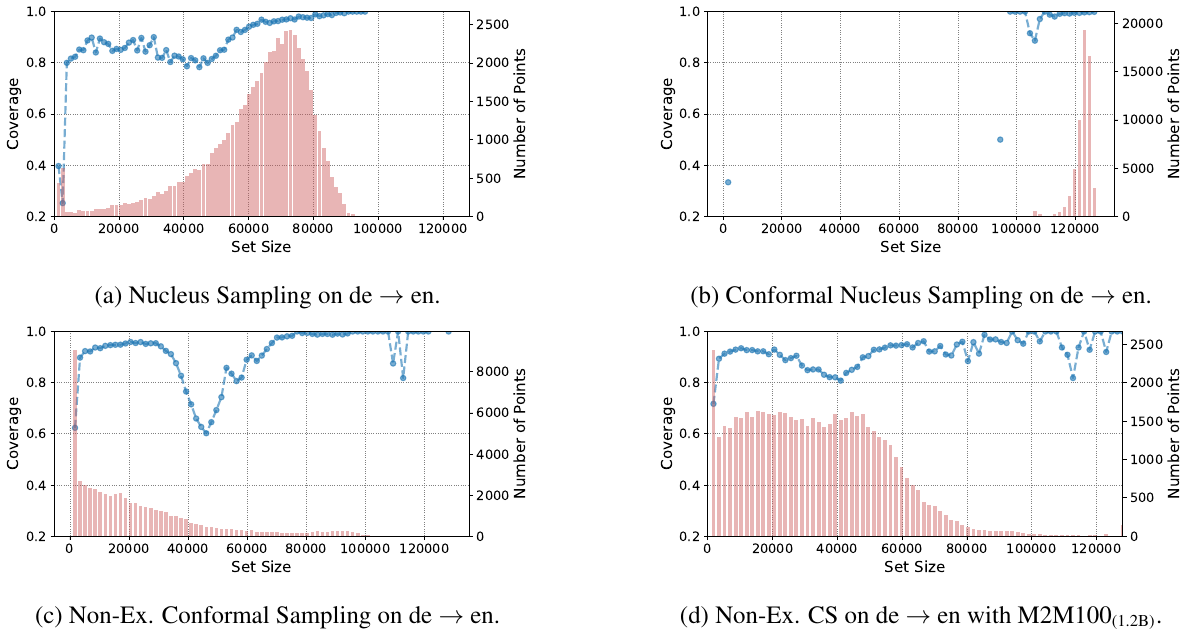
\includegraphics[width=2.676cm]{figures/img/results_gallery/tile_8.png}}};
\draw[black!35,line width=0.35pt] (2.816,-10.110) rectangle (5.492,-12.037);
\node[anchor=north west,text=ACMDarkBlue,font=\tiny\bfseries,inner sep=0] at (2.846,-12.067) {\href{https://arxiv.org/abs/2402.00707}{\adjustbox{max width=2.616cm}{Ulmer et al. 2024b}}};
\node[anchor=north west,text=black!60,font=\tiny,inner sep=0] at (2.846,-12.272) {\href{https://arxiv.org/abs/2402.00707}{Fig. 2, p.~6}};
\node[anchor=north west,inner sep=0] at (5.562,-10.110) {\href{https://arxiv.org/abs/2602.03814}{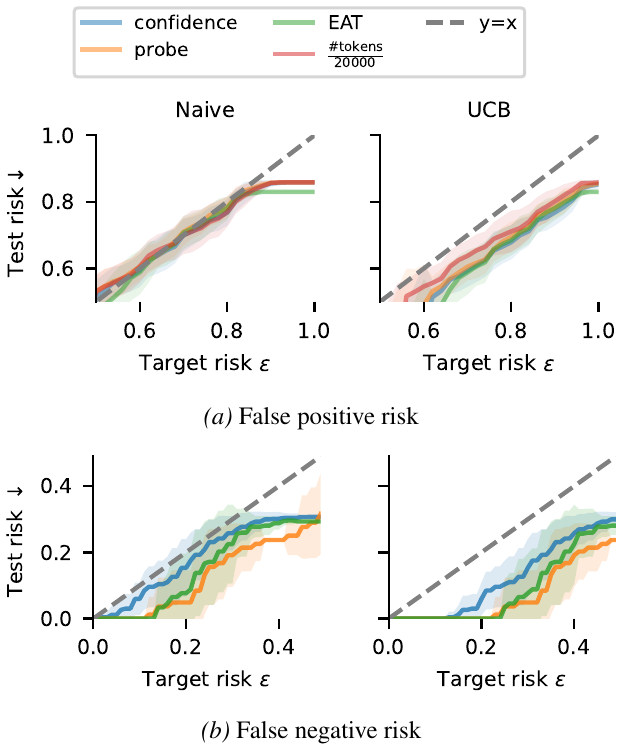
\includegraphics[width=2.676cm]{figures/img/results_gallery/tile_9.png}}};
\draw[black!35,line width=0.35pt] (5.562,-10.110) rectangle (8.238,-12.037);
\node[anchor=north west,text=ACMDarkBlue,font=\tiny\bfseries,inner sep=0] at (5.592,-12.067) {\href{https://arxiv.org/abs/2602.03814}{\adjustbox{max width=2.616cm}{Wang et al. 2026b}}};
\node[anchor=north west,text=black!60,font=\tiny,inner sep=0] at (5.592,-12.272) {\href{https://arxiv.org/abs/2602.03814}{Fig. 4, p.~7}};
\node[anchor=north west,inner sep=0] at (8.308,-10.110) {\href{https://arxiv.org/abs/2406.09714}{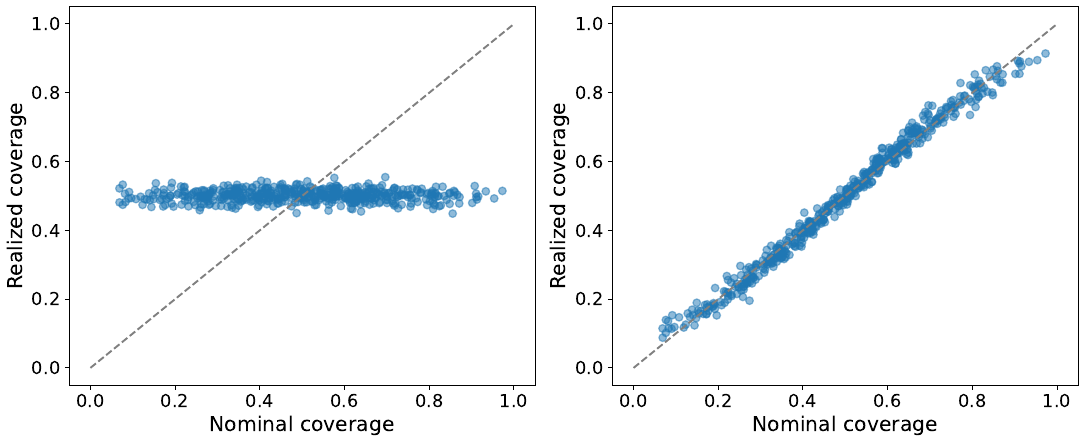
\includegraphics[width=2.676cm]{figures/img/results_gallery/tile_10.png}}};
\draw[black!35,line width=0.35pt] (8.308,-10.110) rectangle (10.984,-12.037);
\node[anchor=north west,text=ACMDarkBlue,font=\tiny\bfseries,inner sep=0] at (8.338,-12.067) {\href{https://arxiv.org/abs/2406.09714}{\adjustbox{max width=2.616cm}{Cherian et al. 2024}}};
\node[anchor=north west,text=black!60,font=\tiny,inner sep=0] at (8.338,-12.272) {\href{https://arxiv.org/abs/2406.09714}{Fig. 8, p.~18}};
\fill[c7C5471] (0,-12.527) rectangle (13.800,-13.027);
\node[anchor=west,text=white,font=\footnotesize\bfseries,inner sep=0] at (0.14,-12.777) {S4 training};
\node[anchor=north west,inner sep=0] at (4.189,-13.097) {\href{https://arxiv.org/abs/2607.04332}{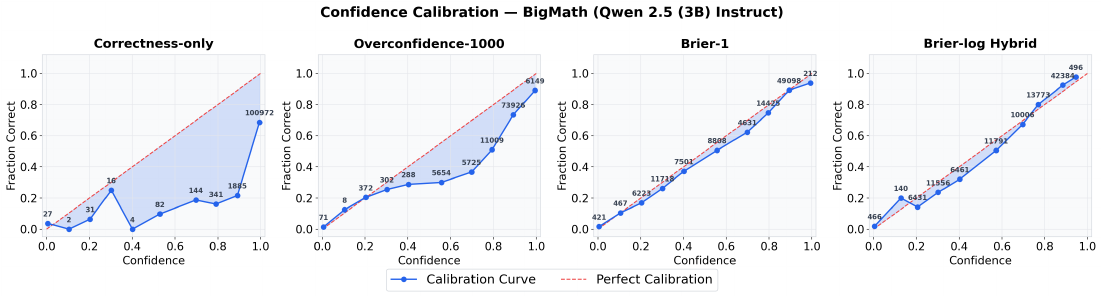
\includegraphics[width=2.676cm]{figures/img/results_gallery/tile_11.png}}};
\draw[black!35,line width=0.35pt] (4.189,-13.097) rectangle (6.865,-15.024);
\node[anchor=north west,text=ACMDarkBlue,font=\tiny\bfseries,inner sep=0] at (4.219,-15.054) {\href{https://arxiv.org/abs/2607.04332}{\adjustbox{max width=2.616cm}{Tan et al. 2026}}};
\node[anchor=north west,text=black!60,font=\tiny,inner sep=0] at (4.219,-15.259) {\href{https://arxiv.org/abs/2607.04332}{Fig. 4, p.~8}};
\node[anchor=north west,inner sep=0] at (6.935,-13.097) {\href{https://arxiv.org/abs/2510.05126}{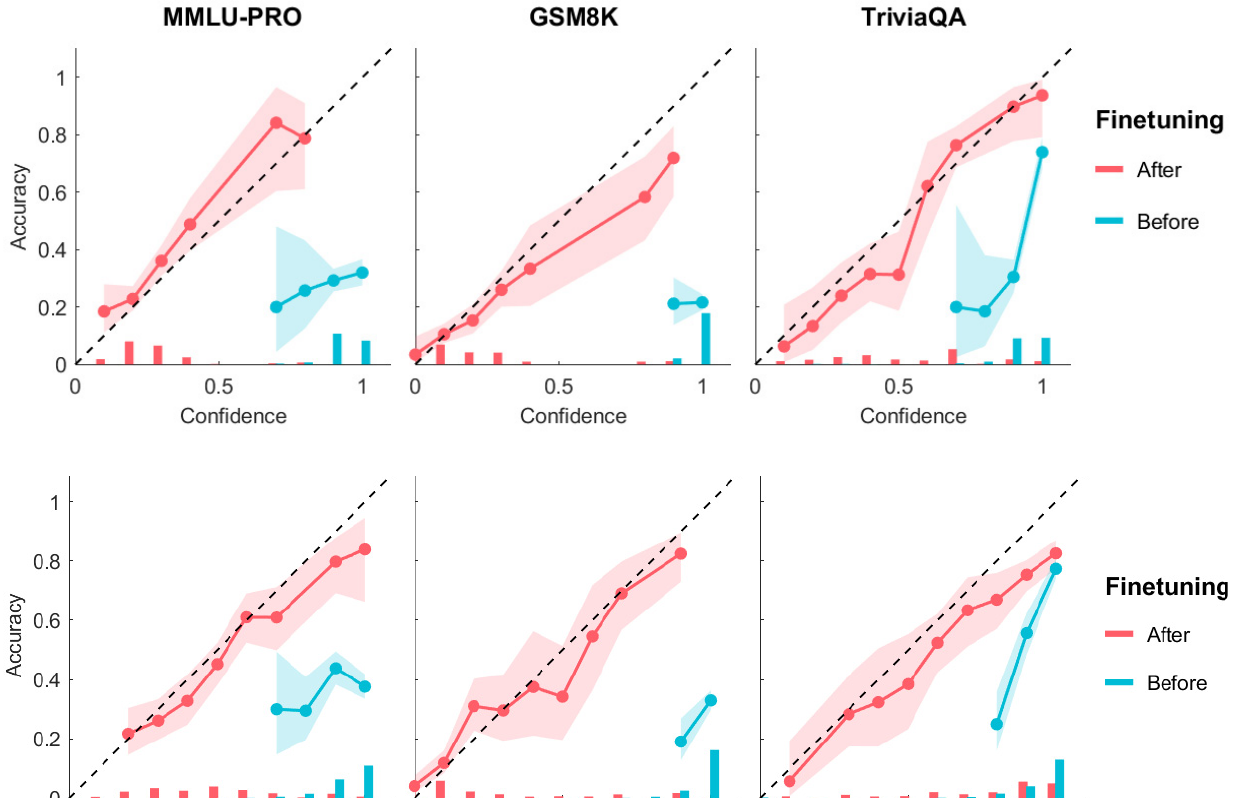
\includegraphics[width=2.676cm]{figures/img/results_gallery/tile_12.png}}};
\draw[black!35,line width=0.35pt] (6.935,-13.097) rectangle (9.611,-15.024);
\node[anchor=north west,text=ACMDarkBlue,font=\tiny\bfseries,inner sep=0] at (6.965,-15.054) {\href{https://arxiv.org/abs/2510.05126}{\adjustbox{max width=2.616cm}{Steyvers et al. 2025a}}};
\node[anchor=north west,text=black!60,font=\tiny,inner sep=0] at (6.965,-15.259) {\href{https://arxiv.org/abs/2510.05126}{Fig. 3, p.~7}};
\fill[c9F3C3C] (0,-15.514) rectangle (13.800,-16.014);
\node[anchor=west,text=white,font=\footnotesize\bfseries,inner sep=0] at (0.14,-15.764) {X consumers and contract};
\node[anchor=north west,inner sep=0] at (2.816,-16.084) {\href{https://arxiv.org/abs/2509.21837}{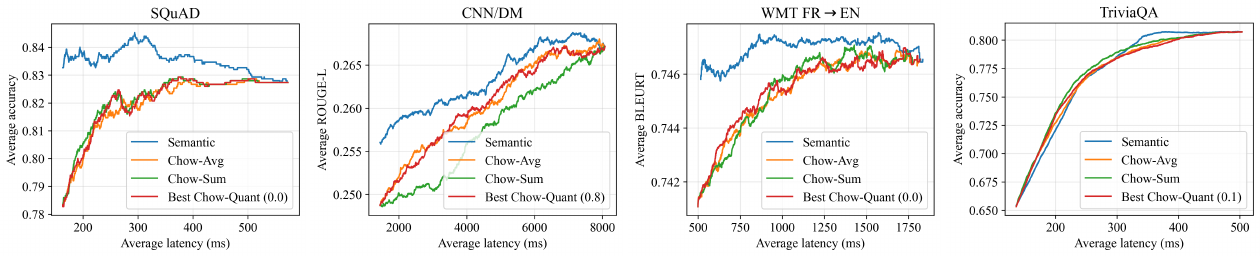
\includegraphics[width=2.676cm]{figures/img/results_gallery/tile_13.png}}};
\draw[black!35,line width=0.35pt] (2.816,-16.084) rectangle (5.492,-18.010);
\node[anchor=north west,text=ACMDarkBlue,font=\tiny\bfseries,inner sep=0] at (2.846,-18.040) {\href{https://arxiv.org/abs/2509.21837}{\adjustbox{max width=2.616cm}{Soiffer et al. 2025}}};
\node[anchor=north west,text=black!60,font=\tiny,inner sep=0] at (2.846,-18.245) {\href{https://arxiv.org/abs/2509.21837}{Fig. 2, p.~5}};
\node[anchor=north west,inner sep=0] at (5.562,-16.084) {\href{https://arxiv.org/abs/2506.11887}{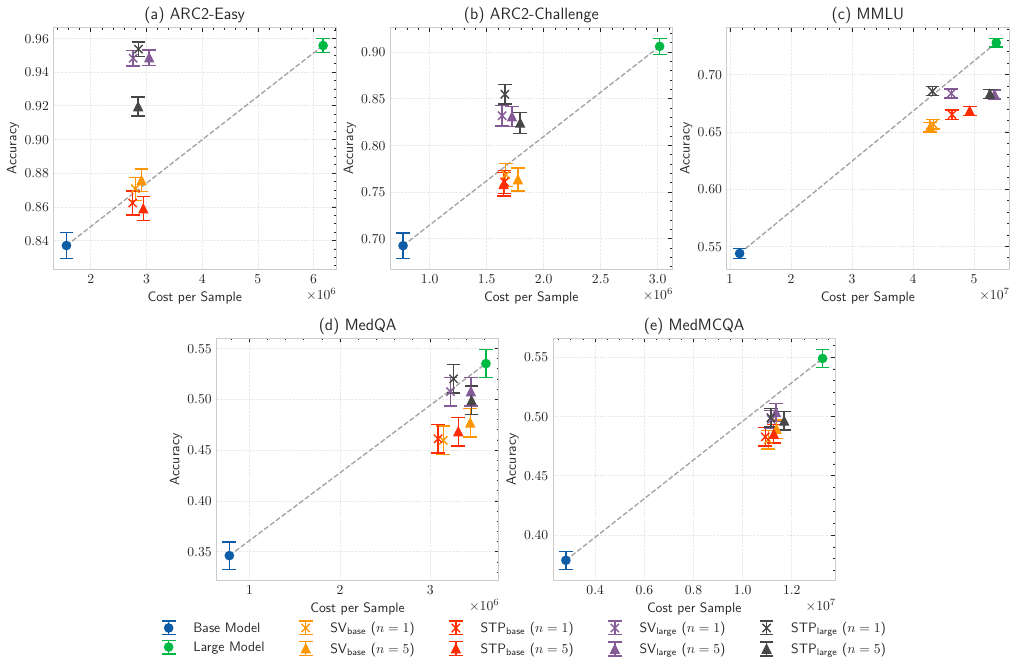
\includegraphics[width=2.676cm]{figures/img/results_gallery/tile_14.png}}};
\draw[black!35,line width=0.35pt] (5.562,-16.084) rectangle (8.238,-18.010);
\node[anchor=north west,text=ACMDarkBlue,font=\tiny\bfseries,inner sep=0] at (5.592,-18.040) {\href{https://arxiv.org/abs/2506.11887}{\adjustbox{max width=2.616cm}{Fanconi and van der Schaar 2025}}};
\node[anchor=north west,text=black!60,font=\tiny,inner sep=0] at (5.592,-18.245) {\href{https://arxiv.org/abs/2506.11887}{Fig. 3, p.~8}};
\node[anchor=north west,inner sep=0] at (8.308,-16.084) {\href{https://arxiv.org/abs/2402.15610}{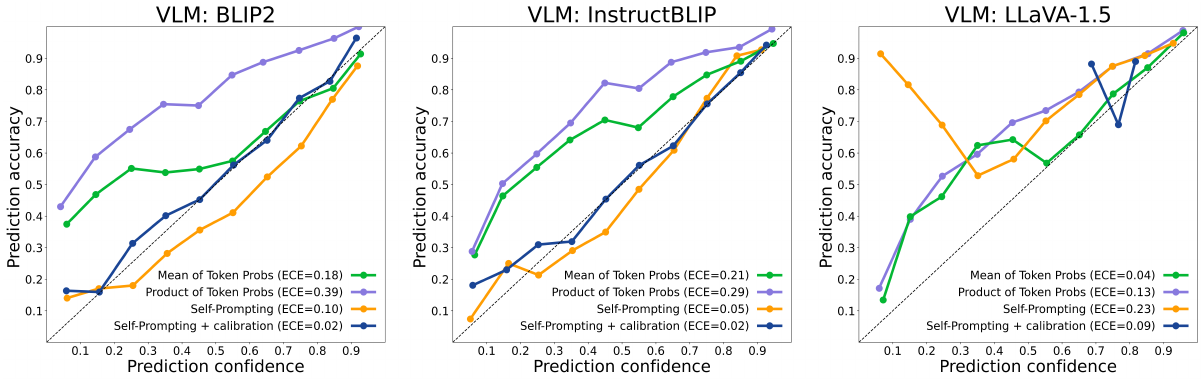
\includegraphics[width=2.676cm]{figures/img/results_gallery/tile_15.png}}};
\draw[black!35,line width=0.35pt] (8.308,-16.084) rectangle (10.984,-18.010);
\node[anchor=north west,text=ACMDarkBlue,font=\tiny\bfseries,inner sep=0] at (8.338,-18.040) {\href{https://arxiv.org/abs/2402.15610}{\adjustbox{max width=2.616cm}{Srinivasan et al. 2024}}};
\node[anchor=north west,text=black!60,font=\tiny,inner sep=0] at (8.338,-18.245) {\href{https://arxiv.org/abs/2402.15610}{Fig. 3, p.~5}};
\end{tikzpicture}}
\caption{\textbf{What calibration looks like in results, by stage.} Each panel shows a whole figure of the cited paper, reproduced under its CC BY licence; its label links to the paper. The selection rule and each panel's figure, page and licence are in Table~\ref{tab:panel_provenance}.}
\Description{A labelled grid of images, each a hyperlink annotated with its system name and source figure number.}
\label{fig:results_gallery}
\end{figure*}


\section{A taxonomy of where calibration enters}
\label{sec:taxonomy}

The taxonomy of Figure~\ref{fig:taxonomy_main} places each work by \emph{where the calibration signal
enters the decision pipeline}. Table~\ref{tab:definitions} (Appendix~\ref{app:definitions}) gives the operational definition of each
stage as a pair: what counts, and the nearest case that does not. Five stages change how the confidence
is produced: the model's own read-off (S0), a post-hoc map (S1), prompt elicitation (S2), extra
inference (S3) and training (S4). The consumers (X) use a confidence without changing how it is
produced, and the theory and analysis works explain when training yields calibration. The last three
rows of the table define the properties recorded for every work: the output contract, the action a
confidence triggers when it is low, and whether a distribution-free guarantee is stated.


\subsection{The core: calibration in the training loss or reward (S4)}
\label{sec:core}

The \nCore core works share one property: a calibration term enters the model's own loss or reward, so
that the model itself, and not a map or a procedure around it, is changed towards calibration. We group
them by \emph{what the training signal scores}. Table~\ref{tab:compare_s4} (Appendix~\ref{app:core}) lists every core work with
its family, output contract, action, guarantee and metric.


\paragraph{T1: supervised calibration objectives (\nTOne works).} The model is fitted to confidence
targets or a calibration loss, without a reward. The oldest works regularise fine-tuning for calibration
in and out of distribution~\citep{kong2020calibrated} or teach a model to state a calibrated numeric or
verbal confidence~\citep{lin2022teaching}. Later work tunes on graded sets of correct and incorrect
answers~\citep{kapoor2024large}, distils sampling-based uncertainty into a single-pass
confidence~\citep{hager2025uncertainty,huang2025efficient}, and trains the stated confidence with a
proper scoring rule as the loss~\citep{li2025conftuner}. One line targets calibration lost elsewhere in
training: after preference alignment~\citep{xiao2025restoring} or after reinforcement
learning~\citep{xiaohu2026know}.

\paragraph{T2: reward-model calibration (\nTTwo works).} The calibrated model is a reward model, usually the one in
the training loop. Calibrated reward modelling counters the overconfidence that preference optimisation
induces~\citep{leng2024taming}; other works expose the reward model's own uncertainty as a
variance~\citep{lou2024uncertaintyaware} or calibrate process reward models by quantile regression, here to set inference compute per
instance~\citep{park2025know}. One reward-model method adds conformal
bounds~\citep{pan2026uncertaintyaware}; it is the only core work that states a distribution-free
guarantee.

\paragraph{T3: calibration rewards on the stated confidence (\nTThree works).} A reward or preference
scores the confidence the model states against the outcome. This is the largest family and, with T5, the newest:
\nTThreeRecent of its \nTThree works appeared in 2025 or 2026, \nTThreeTwentySix of them in 2026. The
rewards include the logarithmic scoring rule~\citep{baniharouni2025rewarding}, a Brier term added to the
correctness reward~\citep{damani2025beyond}, and rewards that let a simulated reader make calibrated
forecasts~\citep{band2024linguistic}. Later work asks which confidence rewards cannot be
hacked~\citep{tan2026on}, compares proper scoring rules as terminal rewards for
forecasters~\citep{turtel2026how}, separates the reasoning and calibration objectives to avoid
gradient conflict~\citep{ma2026decoupling}, and adjusts the probabilities of decision tokens
directly~\citep{yaldiz2026balancing}. Ranking-based confidence rewards~\citep{wang2026calibrationaware}
target discrimination as well as calibration.

\paragraph{T4: abstention and refusal training (\nTFour works).} The signal targets the action: the model
is trained, by supervision or by reward, to abstain when it does not know. Early work builds refusal-aware
fine-tuning data from the questions the model gets wrong~\citep{zhang2023rtuning,yang2023alignment}.
Reinforcement-learning variants use a ternary reward that scores a correct answer above an abstention
and an abstention above an error~\citep{wei2025truthrl,mohamadi2025honesty}, add clarification after a
refusal~\citep{zhai2026abstainr1}, or derive the reward from the model's knowledge
boundary~\citep{gao2026karl}. The family also carries a warning: error-penalised abstention rewards can
collapse a KL-anchored policy to refusing everything~\citep{che2026abstention}.

\paragraph{T5: process- and meaning-level confidence rewards (\nTFive works).} The confidence reward is
given per reasoning step~\citep{he2025mmboundary,wang2026process} or over answers that are equivalent in
meaning~\citep{an2025teaching,yu2026calibrating}, rather than once per final answer.

\paragraph{Theory and analysis (\nTheory works).} These works explain when training yields calibration
and are not counted in the core. Local optimality of a proper loss implies smooth
calibration~\citep{blasiok2023when}; a calibrated language model must hallucinate arbitrary facts at a rate close to the
fraction of such facts seen exactly once in training~\citep{kalai2023calibrated}, and binary-graded training and evaluation
reward guessing~\citep{kalai2025why}. Calibration that emerges from next-token training can break under
reinforcement-learning tuning~\citep{nakkiran2025trained}, and the group standard-deviation
normalisation of GRPO causes overconfidence on stochastic outcomes~\citep{bereket2025uncalibrated}.

\paragraph{Families crossed with the output contract.} The families differ in what they score; they
also differ in what form the trained confidence takes. Of the \nCore core works, \nCoreScore train a
single confidence score, \nCoreFree a free-text answer with a hedge or refusal, and \nCoreTyped the
probability of a typed decision, \coreTypedCalPhrase{} its calibration; \coreOtherPhrase{}. The typed decision appears only in T1 and T3, and abstention training (T4)
is almost entirely free text:

\begin{center}\footnotesize
\begin{tabular}{@{}lrrrrr@{}}
\toprule
Family & Score & Free text & Typed & Other & All \\
\midrule
T1 supervised calibration objectives & \nTOneScore & \nTOneFree & \nTOneTyped & \nTOneOther & \nTOne \\
T2 reward-model calibration & \nTTwoScore & \nTTwoFree & \nTTwoTyped & \nTTwoOther & \nTTwo \\
T3 calibration rewards on the stated confidence & \nTThreeScore & \nTThreeFree & \nTThreeTyped & \nTThreeOther & \nTThree \\
T4 abstention and refusal training & \nTFourScore & \nTFourFree & \nTFourTyped & \nTFourOther & \nTFour \\
T5 process- and meaning-level confidence rewards & \nTFiveScore & \nTFiveFree & \nTFiveTyped & \nTFiveOther & \nTFive \\
\midrule
All core works & \nCoreScore & \nCoreFree & \nCoreTyped & \nCoreOther & \nCore \\
\bottomrule
\end{tabular}\\[2pt]
{\scriptsize Other: a prediction set, or a contract that could not be determined from the paper.}
\end{center}

\noindent The action recorded for a
core work is most often none (\nCoreNoAction works): the trained confidence is reported with the answer,
and the rule that would act on it is left to the user. Abstention is the exception, because the T4
family trains the action itself (\nCoreAbstain core works abstain).

\subsection{The background stages and the consumers}
\label{sec:background}

% GENERATED by build/gen_handtables.py (citations resolved against the verified corpus) -- edit the generator.
\begin{table}[t]
\centering\footnotesize
\setlength{\tabcolsep}{2pt}\renewcommand{\arraystretch}{1.06}\hyphenpenalty=2000\exhyphenpenalty=2000
\caption{\textbf{What each stage yields, costs, guarantees and gets wrong.} The second column is the sense in which the
literature uses ``confidence'' at that stage. A cited phrase is a finding of the cited work; an uncited phrase follows from
the definition of the stage (Table~\ref{tab:definitions}). Only training (S4) changes the model itself; its families are
compared in Table~\ref{tab:compare_s4}.}
\label{tab:stage_limits}
\begin{tabular}{@{}>{\raggedright\arraybackslash}p{0.095\textwidth}>{\raggedright\arraybackslash}p{0.16\textwidth}>{\raggedright\arraybackslash}p{0.12\textwidth}>{\raggedright\arraybackslash}p{0.125\textwidth}>{\raggedright\arraybackslash}p{0.105\textwidth}>{\raggedright\arraybackslash}p{0.165\textwidth}>{\raggedright\arraybackslash}p{0.15\textwidth}@{}}
\toprule
\textbf{Stage} & \textbf{Confidence it yields} & \textbf{Cost: data; inference} & \textbf{Guarantee} & \textbf{Black-box use} & \textbf{Typical failure} & \textbf{Fit for a typed decision} \\
\midrule
S0 read-off & the model's own probability for an option or a true/false judgement \citep{kadavath2022language} & none; none & none & no: needs token probabilities & calibration degrades after post-training \citep{openai2023gpt4} & natural when the options are enumerated and scored \citep{kadavath2022language} \\
S1 post-hoc map & a rescaled, binned or pooled probability \citep{guo2017calibration}, a probe's probability from the hidden states \citep{azaria2023internal}, or an auxiliary model's estimate from the input and output text \citep{ulmer2024calibrating} & held-out data (labels usually; none for a fixed map); negligible & binning: distribution-free \citep{gupta2021distribution}; scaling: none & partly: a map needs the model's scores and a probe its hidden states; an auxiliary model on the text needs neither & a map fitted for one task must be refitted, or predicted by a learned model, for a new one \citep{shen2024thermometer} & good for a fixed label set \citep{guo2017calibration} \\
S2 prompt elicitation & a confidence stated in words or numbers \citep{tian2023just} & none; none if asked with the answer, one more call if asked afterwards & none & yes & stated confidences cluster near the top of the scale \citep{xiong2023can} & the confidence arrives as text and must be parsed \\
S3 sampling & agreement or semantic entropy across sampled answers \citep{wang2022selfconsistency,farquhar2024semantic} & none; several sampled answers per query & none & yes & consistent but wrong answers look confident \citep{tan2025too} & defined over free text; per-option use needs clustering \\
S3 conformal and risk control & a prediction set of options \citep{campos2024conformal}, or a threshold with bounded risk, such as an early exit \citep{schuster2022confident} & a calibration set; a threshold over one pass, or over several sampled answers for sets of generations & coverage $\ge 1-\alpha$ \citep{campos2024conformal}, or a risk bound \citep{angelopoulos2021learn} & either & the guarantee lapses when exchangeability fails \citep{ulmer2024nonexchangeable} & a set returns several options, not one decision; a risk-controlled threshold returns one \\
S4 training & a confidence the model is trained to state or to assign, per option for a typed decision \citep{yaldiz2026balancing} & outcomes or rewards; training compute & none in general; one reward-model method adds conformal bounds \citep{pan2026uncertaintyaware} & no: needs weights & a calibration and accuracy trade-off \citep{yaldiz2026balancing} & can train per-option probabilities directly \citep{yaldiz2026balancing} \\
\bottomrule
\end{tabular}
\end{table}


The stages outside the core are organised in the existing surveys~\citep{li2025survey,shorinwa2025survey}.
Table~\ref{tab:stage_limits} compares them with the core on what each yields, costs, guarantees and gets
wrong, and Table~\ref{tab:landscape} (Appendix~\ref{app:landscape}) lists all \nLandscape works.


The read-off (S0, \nSzero works) needs token probabilities; post-hoc maps (S1, \nSone works) add
temperature scaling, binning~\citep{guo2017calibration} and probes on hidden
states~\citep{azaria2023internal}; prompt elicitation (S2, \nStwo works) works from text
alone~\citep{tian2023just}. Extra inference (S3, \nSthree works) samples several answers and measures
their agreement~\citep{wang2022selfconsistency,farquhar2024semantic}, or calibrates a set or a threshold
with a conformal or risk-control guarantee~\citep{campos2024conformal}; \nGuarSthree of the \nGuar works
that state a guarantee sit here. The consumers (X, \nX works) route, defer, abstain, constrain decoding,
or study how people rely on a stated confidence.

\section{The output contract and the decision loop}
\label{sec:contract}

A confidence is useful to software only if a rule can read it and act. Figure~\ref{fig:decision_loop}
draws the loop that this requires. A decision model receives a state and a \emph{declared} set of
options, assigns a probability to every option in one query, and passes the probabilities to an explicit
action policy. The five stages of the taxonomy differ in where calibration enters this loop; the output
contract determines how directly a rule can act on the result.

% The mechanism figure: where each stage injects calibration. Laid out at the acmsmall text width (no scaling).
\begin{figure}[t]
\centering
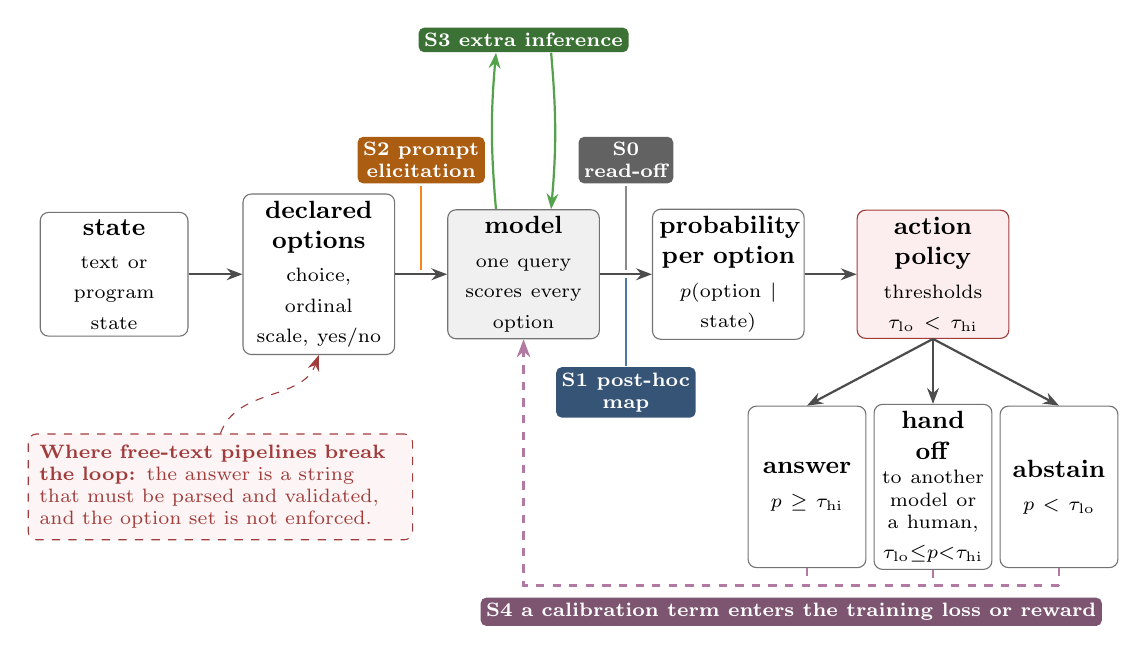
\begin{tikzpicture}[font=\small,
  box/.style={draw=black!55, rounded corners=3pt, align=center, minimum height=13mm,
              text width=17.5mm, inner sep=2.5pt, fill=white},
  act/.style={box, text width=13.2mm, minimum height=20.5mm},
  st/.style={rounded corners=2pt, font=\scriptsize\bfseries, text=white, inner sep=2pt, align=center},
  ar/.style={-{Stealth[length=2mm]}, black!70, line width=0.8pt}]
 % ---- main row ----
 \node[box, text width=17mm] (state)  at (0,0)    {\textbf{state}\\[1pt]{\scriptsize text or program state}};
 \node[box]                (type)   at (2.6,0)  {\textbf{declared options}\\[1pt]{\scriptsize choice, ordinal scale, yes/no}};
 \node[box, fill=black!6]  (model)  at (5.2,0)  {\textbf{model}\\[1pt]{\scriptsize one query scores every option}};
 \node[box]                (prob)   at (7.8,0)  {\textbf{probability per option}\\[1pt]{\scriptsize $p(\text{option}\mid\text{state})$}};
 \node[box, fill=stX!10, draw=stX!70!black] (policy) at (10.4,0) {\textbf{action policy}\\[1pt]{\scriptsize thresholds $\tau_{\mathrm{lo}}<\tau_{\mathrm{hi}}$}};
 \draw[ar] (state) -- (type); \draw[ar] (type) -- (model);
 \draw[ar] (model) -- (prob); \draw[ar] (prob) -- (policy);
 % ---- actions ----
 \node[act] (a1) at (8.8,-2.7) {\textbf{answer}\\[1pt]{\scriptsize $p\ge\tau_{\mathrm{hi}}$}};
 \node[act] (a2) at (10.4,-2.7) {\textbf{hand off}\\[1pt]{\scriptsize to another model or a human,\\ $\tau_{\mathrm{lo}}{\le}p{<}\tau_{\mathrm{hi}}$}};
 \node[act] (a3) at (12.0,-2.7) {\textbf{abstain}\\[1pt]{\scriptsize $p<\tau_{\mathrm{lo}}$}};
 \draw[ar] (policy.south) -- (a1.north); \draw[ar] (policy.south) -- (a2.north); \draw[ar] (policy.south) -- (a3.north);
 % ---- stage tags: where calibration enters ----
 \node[st, fill=stS2txt] at ($(type.east)!0.5!(model.west)+(0,1.45)$) {S2 prompt\\ elicitation};
 \draw[stS2, line width=0.7pt] ($(type.east)!0.5!(model.west)+(0,1.12)$) -- ($(type.east)!0.5!(model.west)+(0,0.05)$);
 \node[st, fill=stS0txt] at ($(model.east)!0.5!(prob.west)+(0,1.45)$) {S0\\ read-off};
 \draw[stS0, line width=0.7pt] ($(model.east)!0.5!(prob.west)+(0,1.12)$) -- ($(model.east)!0.5!(prob.west)+(0,0.05)$);
 \node[st, fill=stS1txt] at ($(model.east)!0.5!(prob.west)+(0,-1.5)$) {S1 post-hoc\\ map};
 \draw[stS1, line width=0.7pt] ($(model.east)!0.5!(prob.west)+(0,-1.17)$) -- ($(model.east)!0.5!(prob.west)+(0,-0.05)$);
 \node[st, fill=stS3txt] (s3) at ($(model.north)+(0,2.15)$) {S3 extra inference};
 \draw[-{Stealth[length=2mm]}, stS3, line width=0.8pt] ($(model.north)+(-0.35,0)$) to[out=95,in=-95] ($(s3.south)+(-0.35,0)$);
 \draw[-{Stealth[length=2mm]}, stS3, line width=0.8pt] ($(s3.south)+(0.35,0)$) to[out=-85,in=85] ($(model.north)+(0.35,0)$);
 % ---- S4: a calibration term in training (a level return bus from the outcomes) ----
 \foreach \a in {a1,a2,a3} \draw[stS4, line width=0.9pt, dashed] (\a.south) -- (\a.south |- 0,-3.95);
 \draw[-{Stealth[length=2.3mm]}, stS4, line width=0.9pt, dashed] (a3.south |- 0,-3.95) -- (model.south |- 0,-3.95) -- (model.south);
 \node[st, fill=stS4txt, anchor=north] at (8.6,-4.1) {S4 a calibration term enters the training loss or reward};
 % ---- where free-text pipelines break the loop ----
 \node[draw=stX!70!black, dashed, rounded corners=3pt, fill=stX!6, text=stX!70!black, align=left,
       text width=46mm, font=\scriptsize, inner sep=4pt] (brk) at (1.35,-2.7)
   {\textbf{Where free-text pipelines break the loop:} the answer is a string that must be parsed
    and validated, and the option set is not enforced.};
 \draw[-{Stealth[length=2mm]}, stX!70!black, dashed] (brk.north) to[out=70,in=250] (type.south);
\end{tikzpicture}
\caption{\textbf{The calibrated decision loop, and where each stage injects calibration.} A decision
model receives a state and a \emph{declared} option set, scores every option in one query,
and hands a probability per option to an explicit action policy. The policy drawn here answers when the probability is high,
hands a less certain case off to another model or a human, and abstains when the probability is low; Table~\ref{tab:definitions}
lists the other low-confidence actions (trigger retrieval, filter the output, adapt compute, return a prediction set). The
five stages of the taxonomy differ in where calibration enters: the model's own read-off
(\textcolor{stS0txt}{\textbf{S0}}), a post-hoc map (\textcolor{stS1txt}{\textbf{S1}}), a prompt that asks for
confidence (\textcolor{stS2txt}{\textbf{S2}}), extra inference such as sampling or a conformal set
(\textcolor{stS3txt}{\textbf{S3}}), or a calibration term in the model's own training loss or reward
(\textcolor{stS4txt}{\textbf{S4}}). The dashed callout marks where free-text generation pipelines break
the loop (Table~\ref{tab:definitions}). Hosted and open typed-decision models (Tables~\ref{tab:jev_hf_ecosystem} and~\ref{tab:jev_decision_index})
expose this interface: a state, declared options (a choice among labels, an ordinal scale or yes/no) and a
probability per option.}
\Description{A left-to-right pipeline: state, declared options, model, probability per option, action policy. The
policy branches down to three actions: answer, hand off to another model or a human, and abstain. Coloured tags mark where calibration
enters: S2 on the prompt arrow, S0 and S1 on the model-to-probability arrow, S3 as a loop around the model, and S4
as a dashed return path from the actions back into the model. A red dashed note says free-text pipelines break the
loop because the answer must be parsed and the option set is not enforced.}
\label{fig:decision_loop}
\end{figure}


We record five contracts, the form of the output that a confidence is attached to
(Figure~\ref{fig:corpus_dist}b). With a \emph{typed decision}, the options are declared before
inference and the model assigns a probability to each, so that the decision and its confidence come
from the same distribution and the action policy can read the probability directly. A \emph{set}
returns several options with a coverage target. With \emph{constrained output}, decoding is restricted
to a grammar or schema; this fixes the form of the answer but not the judgement behind it, and it yields
no confidence of its own. A \emph{score} is one confidence number per answer, stated by the model, read
off its token probabilities or estimated by a separate model. With \emph{free text}, the answer is
free text or a label with no per-answer probability, any confidence is a verbal hedge, an abstention, or
the agreement of several sampled answers, and the answer must be parsed before a rule can use it. A
probability that the model writes out as text, even for a declared outcome, is a score, not a typed
decision. \contractUnknownPhrase{}

\paragraph{Where the typed decision lives.} \nContractTyped works attach the confidence to a typed
decision, and \nTypedCal of them report a calibration metric (ECE, Brier score, NLL or a reliability
diagram) in the main text. Most sit at the earliest stages: \nTypedReadPost at the read-off and the
post-hoc map, where the task is classification or multiple choice and the probability over the declared
options is calibrated directly (\nTypedReadPostCal of them report a calibration metric). \typedOtherStages{} The training core is where the typed decision is rarest: only \nCoreTyped of the \nCore core
works train the probability of a declared option, \coreTypedCalPhrase{} its
calibration. Nearly all the rest train a stated score (\nCoreScore works) or a free-text answer with a hedge or a
refusal (\nCoreFree). Table~\ref{tab:compare_contract} lists every typed work and the \nConstrained
consumers on grammar- or schema-constrained output; the constrained-output works mostly measure
validity, speed, or accuracy under the constraint.

\paragraph{What the confidence triggers.} Across the corpus, most works stop at the confidence: for
\nActNoAction of the \nWorks works no rule or trained behaviour acts on it. Where one does, the
low-confidence action is to abstain (\nActAbstain works), to hand the case off to another model or a
person (\nActHandOff), to return a prediction set (\nActSet), to filter the output (\nActFilter), to
spend more computation (\nActAdapt), or to trigger retrieval (\nActRetrieve). The threshold policy of
Figure~\ref{fig:decision_loop} therefore has to be supplied by whoever deploys the model, and the
calibration of the probability it reads decides how well it works.

\paragraph{Hosted and open decision models.} Some models are now offered with a typed-decision
interface:
unstructured state in, a probability per declared option out. The calibration of one such hosted
model can be checked independently: a third-party evaluation is part of our corpus~\citep{li2026jev},
and a public leaderboard measures the calibration of its chosen option. Appendix~\ref{app:jev} profiles
that model and the open decision models listed with it: the
\nHF repositories that a public model search for its name returns (Table~\ref{tab:jev_hf_ecosystem}),
and the \nDISystems systems of a community leaderboard~\citep{multimodalart2026jevdi} that scores decision models on skill and on the
calibration of the chosen option (Table~\ref{tab:jev_decision_index}).

% AUTO-GENERATED by build/gen_corpus.py from literature/corpus.tsv -- do not hand-edit.
{\footnotesize\setlength{\tabcolsep}{4pt}
\begin{longtable}{@{}>{\raggedright\arraybackslash\hangindent=1em\hangafter=1}p{0.3\textwidth}c>{\raggedright\arraybackslash}p{0.43\textwidth}>{\raggedright\arraybackslash}p{0.1\textwidth}c@{}}
\caption{\textbf{The output contract: 93 works}, selected by a stated rule: every work whose confidence is attached to
a typed decision (contract ``typed'', 65, at any stage), and the X-stage works on grammar- or schema-constrained output
(28). Cal.: \yy{} when the main text reports a calibration metric (ECE, Brier score, NLL or a reliability
diagram); 41 of the 65 typed works do, all 7 in the training core. The constrained-output works
mostly measure validity, speed or accuracy under the constraint. Each work's contribution is in Table~\ref{tab:compare_s4} or
Table~\ref{tab:landscape}. Yr: year of the first public version; Family: the training family (S4) or method family;
Metric: the calibration or confidence metric reported in the main text (ECE, Brier, NLL, AUROC, selective = selective risk or accuracy at a coverage, coverage = achieved coverage of a prediction set or achieved risk under a controlled threshold, multiple = more than one of these (a reliability diagram counts with ECE; PRR with AUROC), other = a different metric, none = no confidence metric). \qq{} = not determinable from the paper.}\label{tab:compare_contract}\\
\toprule \textbf{Work} & \textbf{Yr} & \textbf{Family} & \textbf{Metric} & \textbf{Cal.} \\ \midrule \endfirsthead
\multicolumn{5}{@{}l}{\emph{Table~\thetable, continued}}\\ \toprule \textbf{Work} & \textbf{Yr} & \textbf{Family} & \textbf{Metric} & \textbf{Cal.} \\ \midrule \endhead
\bottomrule \endfoot
\midrule\multicolumn{5}{@{}l}{\textbf{Typed output, S0 read-off} (16)} \\*
\citet{openai2023gpt4} & 2023 & Calibration after alignment & ECE & \yy \\
\citet{huang2026investigating} & 2026 & Calibration after alignment & ECE & \yy \\
\citet{proskurina2026are} & 2026 & Calibration after alignment & ECE & \yy \\
\citet{sanzguerrero2026large} & 2026 & Calibration after alignment & multiple & \yy \\
\citet{desai2020calibration} & 2020 & Empirical studies of read-off calibration & ECE & \yy \\
\citet{dan2021effects} & 2021 & Empirical studies of read-off calibration & ECE & \yy \\
\citet{ahuja2022calibration} & 2022 & Empirical studies of read-off calibration & ECE & \yy \\
\citet{chen2022close} & 2022 & Empirical studies of read-off calibration & ECE & \yy \\
\citet{xiao2022uncertainty} & 2022 & Empirical studies of read-off calibration & multiple & \yy \\
\citet{li2023large} & 2023 & Empirical studies of read-off calibration & multiple & \yy \\
\citet{zhang2023study} & 2023 & Empirical studies of read-off calibration & ECE & \yy \\
\citet{mahaut2024factual} & 2024 & Empirical studies of read-off calibration & other & \ab \\
\citet{joshi2025calibration} & 2025 & Empirical studies of read-off calibration & ECE & \yy \\
\citet{lovering2024language} & 2024 & Likelihood and logit read-off & other & \ab \\
\citet{plaut2024probabilities} & 2024 & Likelihood and logit read-off & multiple & \yy \\
\citet{wang2024my} & 2024 & Likelihood and logit read-off & none & \ab \\
\midrule\multicolumn{5}{@{}l}{\textbf{Typed output, S1 post-hoc map} (24)} \\*
\citet{badhe2026silent} & 2026 & Fixed maps over the read-off & multiple & \yy \\
\citet{zheng2023large} & 2023 & Label-bias and option-prior debiasing & none & \ab \\
\citet{reif2024beyond} & 2024 & Label-bias and option-prior debiasing & none & \ab \\
\citet{han2022prototypical} & 2022 & Learned calibrators & none & \ab \\
\citet{luo2026unlocking} & 2026 & Learned calibrators & multiple & \yy \\
\citet{liu2024calibration} & 2024 & Multicalibration and task-specific recalibration & ECE & \yy \\
\citet{burns2022discovering} & 2022 & Probes and learned confidence heads & other & \ab \\
\citet{azaria2023internal} & 2023 & Probes and learned confidence heads & AUROC & \ab \\
\citet{liu2023cognitive} & 2023 & Probes and learned confidence heads & ECE & \yy \\
\citet{holtzman2021surface} & 2021 & Prompt and context calibration & none & \ab \\
\citet{zhao2021calibrate} & 2021 & Prompt and context calibration & none & \ab \\
\citet{fei2023mitigating} & 2023 & Prompt and context calibration & none & \ab \\
\citet{jiang2023generative} & 2023 & Prompt and context calibration & none & \ab \\
\citet{liusie2023mitigating} & 2023 & Prompt and context calibration & none & \ab \\
\citet{zhou2023batch} & 2023 & Prompt and context calibration & none & \ab \\
\citet{abbas2024enhancing} & 2024 & Prompt and context calibration & ECE & \yy \\
\citet{cho2024token} & 2024 & Prompt and context calibration & none & \ab \\
\citet{gundem2025boosting} & 2025 & Prompt and context calibration & none & \ab \\
\citet{guo2017calibration} & 2017 & Scaling and binning & multiple & \yy \\
\citet{kull2019beyond} & 2019 & Scaling and binning & multiple & \yy \\
\citet{kumar2019verified} & 2019 & Scaling and binning & multiple & \yy \\
\citet{gupta2021distribution} & 2021 & Scaling and binning & ECE & \yy \\
\citet{shen2024thermometer} & 2024 & Scaling and binning & multiple & \yy \\
\citet{luo2025your} & 2025 & Scaling and binning & multiple & \yy \\
\midrule\multicolumn{5}{@{}l}{\textbf{Typed output, S3 extra inference} (11)} \\*
\citet{ling2024uncertainty} & 2024 & Benchmarks and empirical studies & AUROC & \ab \\
\citet{jung2024trust} & 2024 & Conformal abstention, selection and cascades & multiple & \yy \\
\citet{tonolini2024bayesian} & 2024 & Ensembles and cross-model disagreement & multiple & \yy \\
\citet{kruse2025simple} & 2025 & Ensembles and cross-model disagreement & multiple & \yy \\
\citet{schuster2021consistent} & 2021 & Risk control and early exit & coverage & \ab \\
\citet{jazbec2024fast} & 2024 & Risk control and early exit & multiple & \yy \\
\citet{liu2023geval} & 2023 & Sampling consistency & other & \ab \\
\citet{portillowightman2023strength} & 2023 & Sampling consistency & ECE & \yy \\
\citet{becker2024cycles} & 2024 & Sampling consistency & multiple & \yy \\
\citet{yang2024just} & 2024 & Sampling consistency & multiple & \yy \\
\citet{zhang2024calibrating} & 2024 & Sampling consistency & ECE & \yy \\
\midrule\multicolumn{5}{@{}l}{\textbf{Typed output, S4 training} (7)} \\*
\citet{yaldiz2026balancing} & 2026 & T3 calibration rewards on the stated confidence & ECE & \yy \\
\citet{kong2020calibrated} & 2020 & T1 supervised calibration objectives & ECE & \yy \\
\citet{niu2024functionallevel} & 2024 & T1 supervised calibration objectives & ECE & \yy \\
\citet{wang2024blob} & 2024 & T1 supervised calibration objectives & multiple & \yy \\
\citet{xiao2025restoring} & 2025 & T1 supervised calibration objectives & ECE & \yy \\
\citet{xiaohu2026know} & 2026 & T1 supervised calibration objectives & multiple & \yy \\
\citet{jiang2020how} & 2020 & T1 supervised calibration objectives & ECE & \yy \\
\midrule\multicolumn{5}{@{}l}{\textbf{Typed output, X consumers and contract} (7)} \\*
\citet{jitkrittum2023when} & 2023 & Deferral & none & \ab \\
\citet{kondadadi2026l2dclinical} & 2026 & Deferral & none & \ab \\
\citet{li2026jev} & 2026 & Judge calibration & multiple & \yy \\
\citet{varshney2022model} & 2022 & Routing/cascade & none & \ab \\
\citet{ramirez2024optimising} & 2024 & Routing/cascade & none & \ab \\
\citet{zellinger2025rational} & 2025 & Routing/cascade & ECE & \yy \\
\citet{wang2024look} & 2024 & Typed classification & none & \ab \\
\midrule\multicolumn{5}{@{}l}{\textbf{Constrained output, X consumers and contract} (28)} \\*
\citet{scholak2021picard} & 2021 & Constrained decoding & none &  \\
\citet{beurerkellner2022prompting} & 2022 & Constrained decoding & none &  \\
\citet{poesia2022synchromesh} & 2022 & Constrained decoding & none &  \\
\citet{geng2023grammarconstrained} & 2023 & Constrained decoding & none &  \\
\citet{lew2023sequential} & 2023 & Constrained decoding & none &  \\
\citet{willard2023efficient} & 2023 & Constrained decoding & none &  \\
\citet{beurerkellner2024guiding} & 2024 & Constrained decoding & none &  \\
\citet{dong2024xgrammar} & 2024 & Constrained decoding & none &  \\
\citet{geng2024sketchguided} & 2024 & Constrained decoding & none &  \\
\citet{koo2024automatabased} & 2024 & Constrained decoding & none &  \\
\citet{park2024grammaraligned} & 2024 & Constrained decoding & none &  \\
\citet{ugare2024syncode} & 2024 & Constrained decoding & none &  \\
\citet{banerjee2025crane} & 2025 & Constrained decoding & none &  \\
\citet{li2025adaptrack} & 2025 & Constrained decoding & none &  \\
\citet{loula2025syntactic} & 2025 & Constrained decoding & other &  \\
\citet{mundler2025typeconstrained} & 2025 & Constrained decoding & none &  \\
\citet{park2025flexible} & 2025 & Constrained decoding & none &  \\
\citet{reddy2026hidden} & 2026 & Constrained decoding & none &  \\
\citet{tang2023strucbench} & 2023 & Structured-output benchmark & none &  \\
\citet{shorten2024structuredrag} & 2024 & Structured-output benchmark & none &  \\
\citet{tam2024speak} & 2024 & Structured-output benchmark & none &  \\
\citet{xia2024fofo} & 2024 & Structured-output benchmark & none &  \\
\citet{geng2025jsonschemabench} & 2025 & Structured-output benchmark & none &  \\
\citet{yang2025structeval} & 2025 & Structured-output benchmark & none &  \\
\citet{fan2026capacity} & 2026 & Structured-output benchmark & none &  \\
\citet{galeone2026when} & 2026 & Structured-output benchmark & none &  \\
\citet{lee2026format} & 2026 & Structured-output benchmark & none &  \\
\citet{singh2026structured} & 2026 & Structured-output benchmark & none &  \\
\end{longtable}}


\section{A measurable agenda}
\label{sec:future}

Comparing the families of Section~\ref{sec:core} is hard: their works are trained on different base
models and data, report different metrics, and attach the confidence to different
contracts. Table~\ref{tab:future_metrics} proposes seven quantities, each with a definition and a named
public testbed, that would make them comparable, and names the stage or family each one stresses.

% Metric-anchored future agenda. Each metric names a real public testbed.
\begin{table}[tp]
\centering\footnotesize
\renewcommand{\arraystretch}{1.18}
\caption{\textbf{A measurable agenda.} Seven quantities, each with a definition and a named public
testbed, that together would let calibrated decision models be compared on common ground:
calibration of the decision itself, safe abstention, cheap escalation, robustness to shift, the cost
of a typed output contract, the size of a guaranteed set, and a controlled comparison of the training families. Figure~\ref{fig:future_protocol} plots
measured decision ECE (panels a and d) and the target shapes of selective risk and escalation regret
(panels b and c).}
\label{tab:future_metrics}
\begin{tabular}{@{}>{\raggedright\arraybackslash}p{0.16\textwidth}
                  >{\raggedright\arraybackslash}p{0.36\textwidth}
                  >{\raggedright\arraybackslash}p{0.25\textwidth}
                  >{\raggedright\arraybackslash}p{0.15\textwidth}@{}}
\toprule
\textbf{Metric} & \textbf{Definition} & \textbf{Instantiation (testbed)} & \textbf{Stresses} \\
\midrule
Decision ECE & expected calibration error of the probability assigned to the chosen option within a \emph{declared} option set, rather than of a free-text answer & MMLU as four-way choice~\citep{hendrycks2020measuring}; measured for every system on the Jev Decision Index (Table~\ref{tab:jev_decision_index}) & every stage; the main quantity for S4 \\
Selective risk (AURC) & area under the risk-coverage curve obtained by abstaining below a confidence threshold~\citep{geifman2017selective} & LM-Polygraph benchmark~\citep{vashurin2024benchmarking} & S3, action policy \\
Escalation regret & extra cost, relative to the cheapest routing policy that reaches the same accuracy, when escalation to a larger model is triggered by confidence & RouterBench~\citep{hu2024routerbench} & action policy, S1 to S4 \\
Shift calibration gap & decision ECE on held-out subjects minus decision ECE on the subjects used for calibration or training & MMLU subject split, as in~\citet{shen2024thermometer} & S1, S4 \\
Contract cost & schema-validity rate together with the accuracy change relative to unconstrained generation & JSONSchemaBench~\citep{geng2025jsonschemabench}; format-restriction study of~\citet{tam2024speak} & output contract \\
Guarantee tightness & average prediction-set size at a target coverage $1-\alpha$ & multiple-choice sets on MMLU~\citep{hendrycks2020measuring} & S3 (conformal) \\
Family comparison & decision ECE and accuracy of the five training families (T1 to T5) applied to the same base model and data & MMLU as four-way choice~\citep{hendrycks2020measuring}, with the shared-base entries of the Jev Decision Index (Table~\ref{tab:jev_decision_index}) as a reference & S4 families \\
\bottomrule
\end{tabular}
\end{table}


\paragraph{Calibration of the decision itself.} The first quantity, decision ECE, measures the
calibration of the probability a model assigns to the option it chooses within a declared set, rather
than of a free-text answer. It is the main quantity for the training stage, and it is the one quantity
that this survey measures across many systems. Panels (a) and (d) of Figure~\ref{fig:future_protocol}
report it from a community leaderboard of decision models, the Jev Decision
Index~\citep{multimodalart2026jevdi} (\diRelease, a single snapshot of \diDate,
not peer reviewed), which scores \nDISystems systems on skill over \nDIBench decision benchmarks and on
expected calibration error over a 1-in-\nDIOneIn sample of \nDICalBench of them. Skill and calibration
separate on this board: the system ranked first on skill, Jev (\diTopSkill, against \diSecondSkill for the next;
a single point estimate), is not the best calibrated, and
\nDILowerECE of the \nDIOpen open systems have a lower ECE (Table~\ref{tab:jev_decision_index}). The
board reports point estimates without uncertainty intervals and records no cost per decision, so it
measures the first quantity only.

% AUTO-GENERATED by build/gen_fig11.py from literature/notes/jev_decision_index_2026-09-27.json -- do not hand-edit.
\begin{figure}[t]
\centering
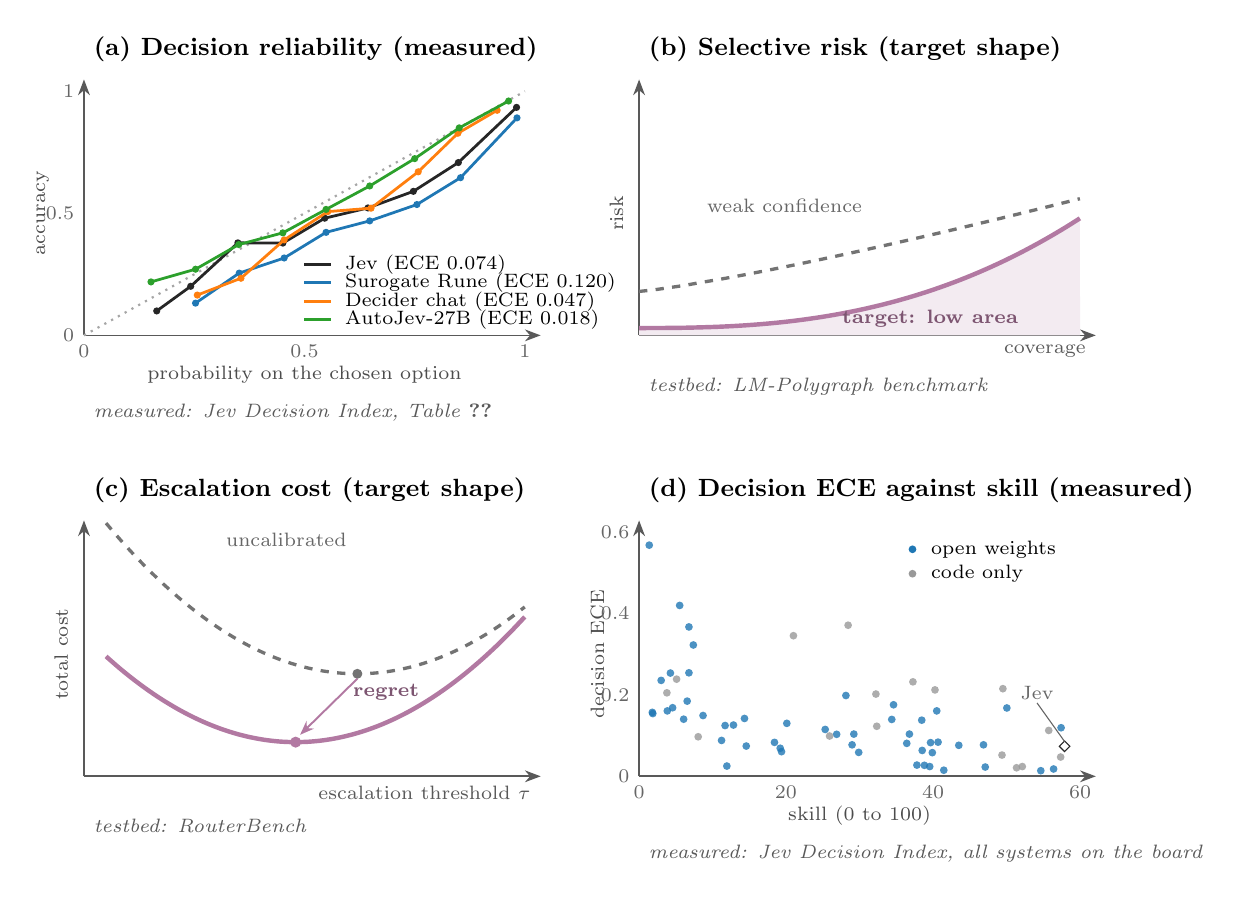
\begin{tikzpicture}[font=\small,
  axis/.style={-{Stealth[length=2mm]}, black!65, line width=0.6pt},
  bad/.style={black!55, line width=1.2pt, dashed},
  good/.style={stS4, line width=1.6pt},
  ttl/.style={font=\small\bfseries, anchor=south west},
  tb/.style={font=\scriptsize\itshape, text=black!65, anchor=north west}]
 \def\W{5.6}\def\H{3.1}\def\G{1.45}\def\V{2.5}
\definecolor{c2}{HTML}{2CA02C}
\definecolor{c1}{HTML}{FF7F0E}
\definecolor{c0}{HTML}{1F77B4}
 \begin{scope}[shift={(0,0)}]
  \node[ttl] at (0,\H+0.25) {(a) Decision reliability (measured)};
  \draw[axis] (0,0) -- (\W+0.2,0); \node[font=\scriptsize,text=black!70] at (0.5*\W,-0.5) {probability on the chosen option};
  \draw[axis] (0,0) -- (0,\H+0.15);
  \node[rotate=90, anchor=south, font=\scriptsize, text=black!70] at (-0.32,0.5*\H) {accuracy};
  \node[font=\scriptsize,text=black!60,below] at (0*\W,0) {0}; \node[font=\scriptsize,text=black!60,left] at (0,0*\H) {0};
  \node[font=\scriptsize,text=black!60,below] at (0.5*\W,0) {0.5}; \node[font=\scriptsize,text=black!60,left] at (0,0.5*\H) {0.5};
  \node[font=\scriptsize,text=black!60,below] at (1*\W,0) {1}; \node[font=\scriptsize,text=black!60,left] at (0,1*\H) {1};
  \draw[black!35, dotted, line width=0.8pt] (0,0) -- (\W,\H);
  \draw[black!85, line width=1.0pt] (0.165*\W,0.100*\H) -- (0.242*\W,0.201*\H) -- (0.349*\W,0.379*\H) -- (0.451*\W,0.378*\H) -- (0.546*\W,0.480*\H) -- (0.644*\W,0.522*\H) -- (0.747*\W,0.590*\H) -- (0.849*\W,0.708*\H) -- (0.981*\W,0.934*\H);
  \fill[black!85] (0.165*\W,0.100*\H) circle (1.3pt); \fill[black!85] (0.242*\W,0.201*\H) circle (1.3pt); \fill[black!85] (0.349*\W,0.379*\H) circle (1.3pt); \fill[black!85] (0.451*\W,0.378*\H) circle (1.3pt); \fill[black!85] (0.546*\W,0.480*\H) circle (1.3pt); \fill[black!85] (0.644*\W,0.522*\H) circle (1.3pt); \fill[black!85] (0.747*\W,0.590*\H) circle (1.3pt); \fill[black!85] (0.849*\W,0.708*\H) circle (1.3pt); \fill[black!85] (0.981*\W,0.934*\H) circle (1.3pt);
  \draw[c0, line width=1.0pt] (0.253*\W,0.132*\H) -- (0.352*\W,0.255*\H) -- (0.454*\W,0.317*\H) -- (0.549*\W,0.422*\H) -- (0.648*\W,0.469*\H) -- (0.755*\W,0.536*\H) -- (0.854*\W,0.646*\H) -- (0.982*\W,0.891*\H);
  \fill[c0] (0.253*\W,0.132*\H) circle (1.3pt); \fill[c0] (0.352*\W,0.255*\H) circle (1.3pt); \fill[c0] (0.454*\W,0.317*\H) circle (1.3pt); \fill[c0] (0.549*\W,0.422*\H) circle (1.3pt); \fill[c0] (0.648*\W,0.469*\H) circle (1.3pt); \fill[c0] (0.755*\W,0.536*\H) circle (1.3pt); \fill[c0] (0.854*\W,0.646*\H) circle (1.3pt); \fill[c0] (0.982*\W,0.891*\H) circle (1.3pt);
  \draw[c1, line width=1.0pt] (0.257*\W,0.165*\H) -- (0.356*\W,0.234*\H) -- (0.454*\W,0.391*\H) -- (0.553*\W,0.507*\H) -- (0.651*\W,0.521*\H) -- (0.758*\W,0.670*\H) -- (0.848*\W,0.828*\H) -- (0.937*\W,0.922*\H);
  \fill[c1] (0.257*\W,0.165*\H) circle (1.3pt); \fill[c1] (0.356*\W,0.234*\H) circle (1.3pt); \fill[c1] (0.454*\W,0.391*\H) circle (1.3pt); \fill[c1] (0.553*\W,0.507*\H) circle (1.3pt); \fill[c1] (0.651*\W,0.521*\H) circle (1.3pt); \fill[c1] (0.758*\W,0.670*\H) circle (1.3pt); \fill[c1] (0.848*\W,0.828*\H) circle (1.3pt); \fill[c1] (0.937*\W,0.922*\H) circle (1.3pt);
  \draw[c2, line width=1.0pt] (0.152*\W,0.219*\H) -- (0.253*\W,0.271*\H) -- (0.351*\W,0.372*\H) -- (0.451*\W,0.420*\H) -- (0.549*\W,0.516*\H) -- (0.648*\W,0.612*\H) -- (0.750*\W,0.724*\H) -- (0.851*\W,0.850*\H) -- (0.963*\W,0.960*\H);
  \fill[c2] (0.152*\W,0.219*\H) circle (1.3pt); \fill[c2] (0.253*\W,0.271*\H) circle (1.3pt); \fill[c2] (0.351*\W,0.372*\H) circle (1.3pt); \fill[c2] (0.451*\W,0.420*\H) circle (1.3pt); \fill[c2] (0.549*\W,0.516*\H) circle (1.3pt); \fill[c2] (0.648*\W,0.612*\H) circle (1.3pt); \fill[c2] (0.750*\W,0.724*\H) circle (1.3pt); \fill[c2] (0.851*\W,0.850*\H) circle (1.3pt); \fill[c2] (0.963*\W,0.960*\H) circle (1.3pt);
  \draw[black!85, line width=1.0pt] (0.5*\W,0.29*\H) -- (0.56*\W,0.29*\H); \node[anchor=west,font=\scriptsize] at (0.57*\W,0.29*\H) {Jev (ECE 0.074)};
  \draw[c0, line width=1.0pt] (0.5*\W,0.21499999999999997*\H) -- (0.56*\W,0.21499999999999997*\H); \node[anchor=west,font=\scriptsize] at (0.57*\W,0.21499999999999997*\H) {Surogate Rune (ECE 0.120)};
  \draw[c1, line width=1.0pt] (0.5*\W,0.13999999999999999*\H) -- (0.56*\W,0.13999999999999999*\H); \node[anchor=west,font=\scriptsize] at (0.57*\W,0.13999999999999999*\H) {Decider chat (ECE 0.047)};
  \draw[c2, line width=1.0pt] (0.5*\W,0.065*\H) -- (0.56*\W,0.065*\H); \node[anchor=west,font=\scriptsize] at (0.57*\W,0.065*\H) {AutoJev-27B (ECE 0.018)};
  \node[tb] at (0,-0.75) {measured: Jev Decision Index, Table~\ref{tab:jev_decision_index}};
 \end{scope}
 \begin{scope}[shift={(\W+\G,0)}]
  \node[ttl] at (0,\H+0.25) {(b) Selective risk (target shape)};
  \draw[axis] (0,0) -- (\W+0.2,0) node[below left, font=\scriptsize] {coverage};
  \draw[axis] (0,0) -- (0,\H+0.15);
  \node[rotate=90, anchor=south, font=\scriptsize, text=black!70] at (-0.08,0.5*\H) {risk};
  \fill[stS4!15] plot[smooth, domain=0:1, samples=30] ({\x*\W},{(0.03+0.45*\x^2.6)*\H}) -- (\W,0) -- (0,0) -- cycle;
  \draw[bad]  plot[smooth, domain=0:1, samples=30] ({\x*\W},{(0.18+0.38*\x^1.2)*\H});
  \draw[good] plot[smooth, domain=0:1, samples=30] ({\x*\W},{(0.03+0.45*\x^2.6)*\H});
  \node[font=\scriptsize, text=black!60] at (0.33*\W,0.53*\H) {weak confidence};
  \node[font=\scriptsize\bfseries, text=stS4txt] at (0.66*\W,0.07*\H) {target: low area};
  \node[tb] at (0,-0.42) {testbed: LM-Polygraph benchmark};
 \end{scope}
 \begin{scope}[shift={(0,-\H-\V)}]
  \node[ttl] at (0,\H+0.25) {(c) Escalation cost (target shape)};
  \draw[axis] (0,0) -- (\W+0.2,0) node[below left, font=\scriptsize] {escalation threshold $\tau$};
  \draw[axis] (0,0) -- (0,\H+0.15);
  \node[rotate=90, anchor=south, font=\scriptsize, text=black!70] at (-0.08,0.5*\H) {total cost};
  \draw[bad]  plot[smooth, domain=0.05:1, samples=30] ({\x*\W},{(0.42+1.9*(\x-0.62)^2)*\H});
  \draw[good] plot[smooth, domain=0.05:1, samples=30] ({\x*\W},{(0.14+1.9*(\x-0.48)^2)*\H});
  \fill[black!55] (0.62*\W,0.42*\H) circle (1.8pt);
  \fill[stS4] (0.48*\W,0.14*\H) circle (2pt);
  \draw[-{Stealth[length=1.8mm]}, stS4, line width=0.7pt] (0.62*\W,0.40*\H) -- (0.49*\W,0.17*\H)
     node[pos=0.25, right, font=\scriptsize\bfseries, text=stS4txt] {regret};
  \node[font=\scriptsize, text=black!60, anchor=west] at (0.30*\W,0.97*\H) {uncalibrated};
  \node[tb] at (0,-0.42) {testbed: RouterBench};
 \end{scope}
 \begin{scope}[shift={(\W+\G,-\H-\V)}]
  \node[ttl] at (0,\H+0.25) {(d) Decision ECE against skill (measured)};
  \draw[axis] (0,0) -- (\W+0.2,0); \node[font=\scriptsize,text=black!70] at (0.5*\W,-0.5) {skill (0 to 100)};
  \draw[axis] (0,0) -- (0,\H+0.15);
  \node[rotate=90, anchor=south, font=\scriptsize, text=black!70] at (-0.32,0.5*\H) {decision ECE};
  \node[font=\scriptsize,text=black!60,below] at (0.000*\W,0) {0};
  \node[font=\scriptsize,text=black!60,below] at (0.333*\W,0) {20};
  \node[font=\scriptsize,text=black!60,below] at (0.667*\W,0) {40};
  \node[font=\scriptsize,text=black!60,below] at (1.000*\W,0) {60};
  \node[font=\scriptsize,text=black!60,left] at (0,0.000*\H) {0};
  \node[font=\scriptsize,text=black!60,left] at (0,0.333*\H) {0.2};
  \node[font=\scriptsize,text=black!60,left] at (0,0.667*\H) {0.4};
  \node[font=\scriptsize,text=black!60,left] at (0,1.000*\H) {0.6};
  \fill[c0, opacity=0.8] (0.957*\W,0.199*\H) circle (1.4pt);
  \fill[black!40, opacity=0.8] (0.956*\W,0.079*\H) circle (1.4pt);
  \fill[c0, opacity=0.8] (0.940*\W,0.030*\H) circle (1.4pt);
  \fill[black!40, opacity=0.8] (0.929*\W,0.188*\H) circle (1.4pt);
  \fill[c0, opacity=0.8] (0.911*\W,0.023*\H) circle (1.4pt);
  \fill[black!40, opacity=0.8] (0.869*\W,0.040*\H) circle (1.4pt);
  \fill[black!40, opacity=0.8] (0.856*\W,0.035*\H) circle (1.4pt);
  \fill[c0, opacity=0.8] (0.834*\W,0.280*\H) circle (1.4pt);
  \fill[black!40, opacity=0.8] (0.825*\W,0.359*\H) circle (1.4pt);
  \fill[black!40, opacity=0.8] (0.823*\W,0.087*\H) circle (1.4pt);
  \fill[c0, opacity=0.8] (0.785*\W,0.038*\H) circle (1.4pt);
  \fill[c0, opacity=0.8] (0.781*\W,0.129*\H) circle (1.4pt);
  \fill[c0, opacity=0.8] (0.725*\W,0.127*\H) circle (1.4pt);
  \fill[c0, opacity=0.8] (0.691*\W,0.025*\H) circle (1.4pt);
  \fill[c0, opacity=0.8] (0.678*\W,0.140*\H) circle (1.4pt);
  \fill[c0, opacity=0.8] (0.675*\W,0.268*\H) circle (1.4pt);
  \fill[black!40, opacity=0.8] (0.671*\W,0.354*\H) circle (1.4pt);
  \fill[c0, opacity=0.8] (0.665*\W,0.097*\H) circle (1.4pt);
  \fill[c0, opacity=0.8] (0.661*\W,0.138*\H) circle (1.4pt);
  \fill[c0, opacity=0.8] (0.659*\W,0.040*\H) circle (1.4pt);
  \fill[c0, opacity=0.8] (0.647*\W,0.045*\H) circle (1.4pt);
  \fill[c0, opacity=0.8] (0.642*\W,0.106*\H) circle (1.4pt);
  \fill[c0, opacity=0.8] (0.641*\W,0.230*\H) circle (1.4pt);
  \fill[c0, opacity=0.8] (0.630*\W,0.046*\H) circle (1.4pt);
  \fill[black!40, opacity=0.8] (0.621*\W,0.387*\H) circle (1.4pt);
  \fill[c0, opacity=0.8] (0.613*\W,0.173*\H) circle (1.4pt);
  \fill[c0, opacity=0.8] (0.607*\W,0.135*\H) circle (1.4pt);
  \fill[c0, opacity=0.8] (0.577*\W,0.293*\H) circle (1.4pt);
  \fill[c0, opacity=0.8] (0.573*\W,0.233*\H) circle (1.4pt);
  \fill[black!40, opacity=0.8] (0.539*\W,0.205*\H) circle (1.4pt);
  \fill[black!40, opacity=0.8] (0.537*\W,0.337*\H) circle (1.4pt);
  \fill[c0, opacity=0.8] (0.498*\W,0.098*\H) circle (1.4pt);
  \fill[c0, opacity=0.8] (0.487*\W,0.173*\H) circle (1.4pt);
  \fill[c0, opacity=0.8] (0.483*\W,0.129*\H) circle (1.4pt);
  \fill[black!40, opacity=0.8] (0.474*\W,0.619*\H) circle (1.4pt);
  \fill[c0, opacity=0.8] (0.469*\W,0.331*\H) circle (1.4pt);
  \fill[c0, opacity=0.8] (0.448*\W,0.172*\H) circle (1.4pt);
  \fill[black!40, opacity=0.8] (0.432*\W,0.165*\H) circle (1.4pt);
  \fill[c0, opacity=0.8] (0.422*\W,0.192*\H) circle (1.4pt);
  \fill[black!40, opacity=0.8] (0.350*\W,0.576*\H) circle (1.4pt);
  \fill[c0, opacity=0.8] (0.335*\W,0.217*\H) circle (1.4pt);
  \fill[c0, opacity=0.8] (0.323*\W,0.101*\H) circle (1.4pt);
  \fill[c0, opacity=0.8] (0.320*\W,0.115*\H) circle (1.4pt);
  \fill[c0, opacity=0.8] (0.307*\W,0.139*\H) circle (1.4pt);
  \fill[c0, opacity=0.8] (0.243*\W,0.124*\H) circle (1.4pt);
  \fill[c0, opacity=0.8] (0.239*\W,0.237*\H) circle (1.4pt);
  \fill[c0, opacity=0.8] (0.214*\W,0.210*\H) circle (1.4pt);
  \fill[c0, opacity=0.8] (0.199*\W,0.042*\H) circle (1.4pt);
  \fill[c0, opacity=0.8] (0.195*\W,0.208*\H) circle (1.4pt);
  \fill[c0, opacity=0.8] (0.187*\W,0.147*\H) circle (1.4pt);
  \fill[c0, opacity=0.8] (0.145*\W,0.249*\H) circle (1.4pt);
  \fill[black!40, opacity=0.8] (0.134*\W,0.162*\H) circle (1.4pt);
  \fill[c0, opacity=0.8] (0.123*\W,0.538*\H) circle (1.4pt);
  \fill[c0, opacity=0.8] (0.113*\W,0.612*\H) circle (1.4pt);
  \fill[c0, opacity=0.8] (0.113*\W,0.424*\H) circle (1.4pt);
  \fill[c0, opacity=0.8] (0.109*\W,0.308*\H) circle (1.4pt);
  \fill[c0, opacity=0.8] (0.101*\W,0.234*\H) circle (1.4pt);
  \fill[c0, opacity=0.8] (0.092*\W,0.700*\H) circle (1.4pt);
  \fill[black!40, opacity=0.8] (0.085*\W,0.398*\H) circle (1.4pt);
  \fill[c0, opacity=0.8] (0.076*\W,0.281*\H) circle (1.4pt);
  \fill[c0, opacity=0.8] (0.071*\W,0.423*\H) circle (1.4pt);
  \fill[c0, opacity=0.8] (0.064*\W,0.268*\H) circle (1.4pt);
  \fill[black!40, opacity=0.8] (0.063*\W,0.342*\H) circle (1.4pt);
  \fill[c0, opacity=0.8] (0.050*\W,0.393*\H) circle (1.4pt);
  \fill[c0, opacity=0.8] (0.031*\W,0.257*\H) circle (1.4pt);
  \fill[c0, opacity=0.8] (0.030*\W,0.262*\H) circle (1.4pt);
  \fill[c0, opacity=0.8] (0.023*\W,0.947*\H) circle (1.4pt);
  \node[diamond, draw=black!85, fill=white, minimum size=4pt, inner sep=0pt] at (0.965*\W,0.123*\H) {};
  \draw[black!60] (0.965*\W,0.123*\H+0.06) -- (0.965*\W-0.35,0.123*\H+0.55) node[anchor=south,font=\scriptsize,inner sep=1pt] {Jev};
  \fill[c0] (0.62*\W,0.93*\H) circle (1.4pt); \node[anchor=west,font=\scriptsize] at (0.64*\W,0.93*\H) {open weights};
  \fill[black!40] (0.62*\W,0.83*\H) circle (1.4pt); \node[anchor=west,font=\scriptsize] at (0.64*\W,0.83*\H) {code only};
  \node[tb] at (0,-0.75) {measured: Jev Decision Index, all systems on the board};
 \end{scope}
\end{tikzpicture}
\caption{\textbf{A measurable agenda, partly measured.} Decision ECE is the expected calibration error of the probability
a model places on its chosen option (Table~\ref{tab:future_metrics}). Panels (a) and (d) come from one community leaderboard,
the Jev Decision Index~\citep{multimodalart2026jevdi} (release 0.2.1, a single snapshot of 2026-09-27; not peer reviewed): skill
is its chance-normalised score over 38 decision benchmarks (0 to 100), ECE is computed on a
1-in-6 sample of 32 of them, and all values
are point estimates without uncertainty intervals. (a)~Reliability measured on the Jev Decision Index
(Table~\ref{tab:jev_decision_index}) for Jev and the three open systems with the highest skill; each point is a confidence
bin, and bins holding under 1\% of answers are omitted. (b)~Selective risk and (c)~escalation regret are drawn as target
shapes, not measured results: purple marks the target, grey dashed a typical baseline, and the named testbeds are in
Table~\ref{tab:future_metrics}. (d)~Decision ECE against skill for Jev and the 67 open systems on the board;
lower right is better. The board records no cost per decision, so skill is used as the horizontal axis.}
\Description{Four plots in a two by two grid. Top left: measured reliability curves of Jev and three open decision models
against the diagonal. Top right and bottom left: schematic target shapes for selective risk and escalation cost. Bottom
right: a scatter of calibration error against skill for every system on the Jev Decision Index, with Jev marked by a hollow diamond.}
\label{fig:future_protocol}
\end{figure}


\paragraph{Acting on the confidence.} Selective risk and escalation regret measure what the confidence
buys once a rule acts on it: the error that remains after abstaining below a
threshold~\citep{geifman2017selective}, and the extra cost of escalating to a larger model when a
cheaper policy would reach the same accuracy~\citep{hu2024routerbench}. Panels (b) and (c) of
Figure~\ref{fig:future_protocol} draw their target shapes; they are not measured results.

\paragraph{Shift, contract and guarantee.} The shift calibration gap asks whether a map or a trained
confidence stays calibrated on subjects it was not fitted on~\citep{shen2024thermometer}. The contract
cost asks what a constrained or typed output costs in accuracy relative to free
generation~\citep{geng2025jsonschemabench,tam2024speak}. Guarantee tightness asks how large a prediction
set must be to reach a target coverage. The last quantity, a comparison of the five training families on
the same base model and data, is the controlled experiment that would say which training signal to prefer.

\FloatBarrier   % every main-body float appears before Limitations and the references
\section{Limitations}
\label{sec:limitations}

\paragraph{Search.} The query strings and the number of records screened were not recorded, so the
search cannot be replayed exactly; Figure~\ref{fig:prisma} marks those stages instead of estimating
them. The \nStreams searches were run on one day, \searchDate, and the last year of the corpus is
partial. Works placed only through the literature they cite, or not indexed by the searches, may be
missing.

\paragraph{Placement.} Stage, family and the per-work fields were assigned by reading each paper and were
then checked against the papers in several review rounds and corrected where they disagreed. Some
works sit on a boundary, for example a method that both trains a confidence and acts on it, and another
reader could place them differently. The one-value-per-work fields (contract, action, metric) record the
main contribution and the main text, not every variant a paper reports.

\paragraph{Evidence.} The families are compared as the papers report them, on different base models,
data and metrics; no claim here ranks one family above another. The leaderboard behind
Figure~\ref{fig:future_protocol} and Table~\ref{tab:jev_decision_index} is a single snapshot, is not peer
reviewed, and reports point estimates without uncertainty intervals. The gallery figures are limited to
papers whose licence permits reuse, so they show only part of each stage.

\section{Conclusion}
\label{sec:conclusion}

Calibration of language models, long estimated after the fact, is increasingly also trained into the
model. We organised \nWorks works by where calibration enters the decision pipeline, and the
\nCore training-stage works by what the training signal scores: supervised calibration objectives,
reward-model calibration, calibration rewards on the stated confidence, abstention and refusal training,
and process- and meaning-level confidence rewards. Crossing that typology with the output contract shows
where the field is thin: the typed decision, whose probability is the very interface a program acts
on, is calibrated after the fact in many works but trained in only \nCoreTyped of the \nCore training works;
most train a stated score or a free-text hedge or refusal. The seven quantities of
Table~\ref{tab:future_metrics} would let the families be compared on common ground, and the first of
them can already be measured.


\section*{Competing interests}
The authors have no financial or other relationship with TypeSafe AI, the maker of Jev, or with the
maintainer of the Jev Decision Index. Jev is profiled as one instance of a hosted typed-decision model.

\bibliographystyle{ACM-Reference-Format}
\bibliography{refs,corpus}

% Appendices follow the References (acmart convention); start on a fresh page.
\clearpage
\appendix
\section{Hosted and open decision models}
\label{app:jev}

Jev is a hosted model from TypeSafe AI, released on 15 September 2026~\citep{almeida2026introducing}, that returns a probability for each
declared option: a typed decision in the sense of Table~\ref{tab:definitions}. This appendix records two
public views of the models around it, both taken on \diDate. Neither is peer reviewed, and neither is
used to rank the training families of Section~\ref{sec:core}. Jev itself is not one of the \nWorks works in
our corpus, and its base model is not disclosed (Table~\ref{tab:jev_decision_index}); this appendix describes
only its interface and its measured calibration.

Table~\ref{tab:jev_hf_ecosystem} classifies the repositories returned by a public model search for its
name. Of the \nHF repositories, \nHFNameOnly only share the name, \nHFUnverified could not be verified, and \nHFClassified were classified
from their model cards and file lists; \nHFTrained contain newly trained weights, and general-purpose
models with their copies account for \nHFGeneralPct of downloads. A name search is a poor census of
decision models: of the \nDIOpenWeights open systems with released weights on the leaderboard of
Table~\ref{tab:jev_decision_index}, it returns \nDIFoundByName.

Table~\ref{tab:jev_decision_index} lists the top of that leaderboard, the Jev Decision
Index~\citep{multimodalart2026jevdi} (\diRelease), which scores
\nDISystems systems on skill over \nDIBench decision benchmarks and on the calibration of the chosen
option; Figure~\ref{fig:future_protocol} plots the same data.

\renewcommand{\thetable}{A\arabic{table}}\setcounter{table}{0}   % Appendix A tables: A1, A2
% AUTO-GENERATED by build/gen_jev_market.py from literature/notes/jev_hf_268.tsv -- do not hand-edit.
\begin{table}[tp]
\centering\footnotesize
\renewcommand{\arraystretch}{1.18}
\caption{\textbf{Repositories returned by the Hugging Face model search for ``jev'', by application} (snapshot of
2026-09-27). \href{https://typesafe.ai/blog/introducing-system-one-models-and-jev}{Jev} is a hosted model from TypeSafe AI, released on 2026-09-15~\citep{almeida2026introducing},
that returns a probability for each declared option (a typed decision, Table~\ref{tab:definitions}). Of the 268
repositories the search returns, 76 only share the name (75 predate Jev) and 4
could not be verified (empty, without a card, or gated with no public card metadata); the remaining 188 are classified here from their
model cards and file lists (for a gated repository, from its public card metadata), with an application category taking
precedence over a language one. Downloads are over the last
30 days. 137 repositories contain newly trained weights; the 38 copies, ports and packages add
none (the 6 mirrors contain their source's weight files byte for byte). General-purpose models and the
copies of them account for 87\% of the 41,653 downloads in the table. A name search misses most decision models: of the
51 open systems with released weights on the Jev Decision Index (Table~\ref{tab:jev_decision_index}), it returns 4.}
\Description{A table with one row per application category of the repositories returned by the Hugging Face search for jev,
giving the number of repositories, their downloads over thirty days and linked example repositories. General-purpose typed-decision models are
the largest group, followed by research checkpoints and copies.}
\label{tab:jev_hf_ecosystem}
\begin{tabular}{@{}>{\raggedright\arraybackslash}p{0.24\textwidth}rr>{\raggedright\arraybackslash}p{0.45\textwidth}@{}}
\toprule
\textbf{Category} & \textbf{Repositories} & \textbf{Downloads} & \textbf{Examples} \\
\midrule
General-purpose typed-decision model & 55 & 19,655 & \href{https://huggingface.co/alibiserikbay/JevK5}{JevK5}, \href{https://huggingface.co/ZefanCai/Open-Jev-9B}{Open-Jev-9B}, \href{https://huggingface.co/com-kotobalabs/open-jev-deberta-v3-large}{open-jev-deberta}, \href{https://huggingface.co/lostargon/Tiny-Jev}{Tiny-Jev}, \href{https://huggingface.co/chaoliangUNSW/Jev-Style-0.8B-Decision-v3}{Jev-Style v3} \\
Research and ablation checkpoints & 45 & 212 & \href{https://huggingface.co/Praveenrajus/jevify-qwen3.5-4b-readout-coh}{jevify} (31-checkpoint readout series), \href{https://huggingface.co/JonesLin/next-jev-stage1-cot}{next-jev} (latent-workspace study), \href{https://huggingface.co/ryandcunha/mmbu-jev-qwen3-0.6b-closed}{mmbu-jev} (closed-set vs free-text) \\
Copy, port or package (no new training) & 38 & 18,640 & \href{https://huggingface.co/mradermacher/JEV-9B-GGUF}{JEV-9B-GGUF} (GGUF), \href{https://huggingface.co/Ruiruiz30/Jev-Omni-MLX-4bit}{Jev-Omni-MLX-4bit} (MLX), \href{https://huggingface.co/onnx-community/open-jev-deberta-v3-large-ONNX}{open-jev-deberta-ONNX} (ONNX), \href{https://huggingface.co/liodon-ai/JevK5-FP8}{JevK5-FP8} (FP8), \href{https://huggingface.co/junetask/Open-Jev-9B}{junetask/Open-Jev-9B} (a mirror) \\
No newly trained model (recipe, runtime, code or data) & 11 & 0 & \href{https://huggingface.co/NicolaiMTLassen/bonzi-8b-v1-jev}{bonzi} (recipes), \href{https://huggingface.co/Meanblock/JEV-CPU}{JEV-CPU} (code), \href{https://huggingface.co/SargeDev/jev-distill-corpus}{jev-distill-corpus} (dataset) \\
Agents, tools and safety & 10 & 1,005 & \href{https://huggingface.co/samatv256/mini-Jev}{mini-Jev} (tool routing), \href{https://huggingface.co/nicolasembleton/mini-jev-minicpm5-2b-shell-safety-phase1b-merged}{Mini-Jev shell-safety}, \href{https://huggingface.co/SargeDev/jev-gate-student-b}{Jev-Gate} (memory gating), \href{https://huggingface.co/atmaneayoub/jev-ar}{jev-ar} (Gulf-Arabic intent routing) \\
Domain application & 10 & 152 & \href{https://huggingface.co/Nebulaw1/jev-qwen3.5-4b-legal-lora}{jev-legal} (Chinese legal), \href{https://huggingface.co/mogita/jev-decider-qwen3-4b}{jev-decider} (bank transactions), \href{https://huggingface.co/guzus/jev-nyotti}{jev-nyotti} (BTC trading), \href{https://huggingface.co/wendellperbar/serigy-jev}{Serigy-Jev} (PT-BR fake news), \href{https://huggingface.co/sdmlai/nano-jev}{Nano-Jev} (RAG) \\
Language-specific & 7 & 1,010 & \href{https://huggingface.co/argos1111/modernbert-ja-310m-jev}{modernbert-ja-jev} (Japanese), \href{https://huggingface.co/wwydmanski/bielik-minitron-jev-v0.3}{bielik-minitron-jev} (Polish), \href{https://huggingface.co/nouton/jev-ru-4b-lora-v2}{Jev-RU} (Russian, Ukrainian, Belarusian) \\
Multimodal or vision & 5 & 594 & \href{https://huggingface.co/akhilaaa3/Jev-Omni}{Jev-Omni} (text, image, audio, video), \href{https://huggingface.co/SeanLiu/Jev-Vision}{Jev-Vision}, \href{https://huggingface.co/Fr0zencr4nE/jev-spatial}{Jev-Spatial} \\
Games and control & 5 & 156 & \href{https://huggingface.co/SUPER321/jevflash-doom-basic-0.6b}{JevFlash} (Doom), \href{https://huggingface.co/bzantium/gemma-3-270m-jev}{gemma-3-270m-jev} (ViZDoom), \href{https://huggingface.co/zwh20081/hoi4-jevai}{JevAI} (Hearts of Iron IV mod) \\
Embeddings trained on typed-decision questions & 2 & 229 & \href{https://huggingface.co/HIT-TMG/JevEmbed-KaLM-Embedding-V2.5}{JevEmbed-KaLM}, \href{https://huggingface.co/HIT-TMG/JevEmbed-Qwen3-Embedding-0.6B}{JevEmbed-Qwen3} \\
\midrule
\textbf{Total} & \textbf{188} & \textbf{41,653} & \\
\bottomrule
\end{tabular}
\end{table}

% AUTO-GENERATED by build/gen_jev_market.py from literature/notes/jev_decision_index_2026-09-27.json -- do not hand-edit.
\begin{table}[tp]
\centering\footnotesize
\setlength{\tabcolsep}{3.5pt}
\caption{\textbf{Jev and open decision models on the Jev Decision Index}: ranks 1 to 15 of the 68
systems on the \href{https://huggingface.co/spaces/multimodalart/jev-decision-index}{Jev Decision Index}~\citep{multimodalart2026jevdi} (release 0.2.1,
data of 2026-09-27). Skill is chance-normalised (0 to 100) over the same 38-benchmark
panel for every system, and unanswered requests count as wrong. ECE is measured on a one-in-6
sample of 32 benchmarks with a per-field right answer. The board reports point estimates
without uncertainty intervals. Base model and method are as recorded by the board: full fine-tune, a low-rank adapter (LoRA), a trained head or adapter over a frozen model, inference only (prompting or decoding over unchanged weights) or a hosted API. Names link to the
model's Hugging Face repository, or to its code where no weights are released. Jev ranks 1 on skill;
across the whole board, 17 of the 67 open systems have a lower ECE than Jev.}
\Description{A table of the fifteen highest-ranked decision models on the Jev Decision Index, with base model, adaptation method,
skill score and expected calibration error.}
\label{tab:jev_decision_index}
\begin{tabular}{@{}rlllrr@{}}
\toprule
\textbf{Rank} & \textbf{System} & \textbf{Base model} & \textbf{Method} & \textbf{Skill} & \textbf{ECE} \\
\midrule
1 & \href{https://typesafe.ai/blog/introducing-system-one-models-and-jev}{Jev 1.13 (TypeSafe AI, hosted)} & not disclosed & hosted API & 57.91 & 0.074 \\
2 & \href{https://huggingface.co/surogate/rune-26b-a4b-GGUF}{Surogate Rune 26B-A4B v3 [bf16]} & gemma-4-26B-A4B-it & full fine-tune & 57.44 & 0.120 \\
3 & \href{https://github.com/Mapika/decider}{Decider chat · Gemma-4-31B} & gemma-4-31B & inference only & 57.33 & 0.047 \\
4 & \href{https://huggingface.co/denis-pplx/autojev-27b}{AutoJev-27B} & Qwen3.8-27B & full fine-tune & 56.40 & 0.018 \\
5 & \href{https://github.com/featherless-ai/simple-jev}{simple-jev · Qwen3.8-27B (featherless)} & Qwen3.8-27B & inference only & 55.74 & 0.113 \\
6 & \href{https://huggingface.co/frontier-infra/jebadiah-27b}{Jebadiah 27B} & Qwen3.8-27B & LoRA & 54.67 & 0.014 \\
7 & \href{https://github.com/kshetrajna12/reflex}{reflex 27B [FP8 · wide choice]} & Qwen3.8-27B & inference only & 52.16 & 0.024 \\
8 & \href{https://github.com/Mapika/decider}{Decider chat · Qwen3.6-27B} & Qwen3.6-27B & inference only & 51.35 & 0.021 \\
9 & \href{https://huggingface.co/EldanRing/Winnow-12B}{Winnow-12B [Q8\_0]} & gemma-4-12B & LoRA & 50.02 & 0.168 \\
10 & \href{https://github.com/JoshuaSP/open-jev}{JoshuaSP diffusiongemma (open-jev)} & diffusiongemma-26B-A4B-it & inference only & 49.47 & 0.216 \\
11 & \href{https://github.com/kikoncuo/jevfire}{Jevfire} & Qwen3.8-27B & inference only & 49.37 & 0.052 \\
12 & \href{https://huggingface.co/Mapika/decider-35b-a3b-nvfp4}{Decider 35B-A3B [NVFP4]} & Qwen3.5-35B-A3B-Base & full fine-tune & 47.11 & 0.023 \\
13 & \href{https://huggingface.co/kirp/jpt-9b}{JPT-9B} & Qwen3.5-9B-Base & LoRA & 46.89 & 0.077 \\
14 & \href{https://huggingface.co/llm-semantic-router/Decision-1.0-Lux-9B}{Decision 1.0 Lux} & Qwen3.5-9B-Base & head or adapter & 43.49 & 0.076 \\
15 & \href{https://huggingface.co/juspay/xor}{Xor} & Qwen3.6-35B-A3B & full fine-tune & 41.48 & 0.015 \\
\bottomrule
\end{tabular}
\end{table}



\section{Provenance of the gallery panels}
\renewcommand{\thetable}{B\arabic{table}}\setcounter{table}{0}   % Appendix B tables: B1
\label{app:provenance}

Table~\ref{tab:panel_provenance} gives, for every panel of Figures~\ref{fig:hero_collage},
\ref{fig:method_gallery} and~\ref{fig:results_gallery}, the source figure and page in the cited paper and
the licence under which it is reproduced, together with the rule by which panels were chosen.

% AUTO-GENERATED by build/gallery.py compile -- provenance of every gallery panel.
\begin{table}[htp]
\centering\footnotesize
\caption{\textbf{Provenance of the gallery panels} in Figures~\ref{fig:hero_collage}, \ref{fig:method_gallery}
and~\ref{fig:results_gallery}: the source figure and page in the cited arXiv paper, and the licence under which it is
reproduced. Panels are chosen by a fixed rule: only papers whose licence permits reuse (CC BY); per stage, one panel per method family (per training family at S4), taking the largest families first and, in each, the newest figure that legibly shows the method or a result, at most 3 per stage; families with no reusable figure that legibly shows the method or a result are skipped. Figure~\ref{fig:method_gallery}: No reusable figure passed the visual check for S0 read-off. At S4, T5 had a figure but was cut by the cap of 3. T2 has no reusable figure that passed the check. Figure~\ref{fig:results_gallery}: At S4, T2, T4, T5 have no reusable figure that passed the check.}
\label{tab:panel_provenance}
\begin{tabular}{@{}lllll@{}}
\toprule
\textbf{Work} & \textbf{Source} & \textbf{Panel} & \textbf{Licence} & \textbf{Used in Fig.} \\
\midrule\multicolumn{5}{@{}l}{\textbf{S0 read-off}} \\\nopagebreak
\citet{sanzguerrero2026large} & \href{https://arxiv.org/abs/2606.03437}{arXiv:2606.03437} & Fig. 4, p.~6 & CC BY 4.0 & 9 \\
\citet{stengeleskin2022calibrated} & \href{https://arxiv.org/abs/2211.07443}{arXiv:2211.07443} & Fig. 1, p.~6 & CC BY 4.0 & 1, 9 \\
\midrule\multicolumn{5}{@{}l}{\textbf{S1 post-hoc map}} \\\nopagebreak
\citet{gundem2025boosting} & \href{https://arxiv.org/abs/2505.23783}{arXiv:2505.23783} & Fig. 2, p.~5 & CC BY 4.0 & 8 \\
\citet{liu2023cognitive} & \href{https://arxiv.org/abs/2312.03729}{arXiv:2312.03729} & Fig. 2, p.~3 & CC BY 4.0 & 9 \\
\citet{lu2026diagnosing} & \href{https://arxiv.org/abs/2607.16799}{arXiv:2607.16799} & Fig. 1, p.~2 & CC BY 4.0 & 1, 8 \\
\citet{luo2025your} & \href{https://arxiv.org/abs/2505.16690}{arXiv:2505.16690} & Fig. 1, p.~3 & CC BY 4.0 & 9 \\
\citet{luo2026unlocking} & \href{https://arxiv.org/abs/2601.04277}{arXiv:2601.04277} & Fig. 1, p.~2 & CC BY 4.0 & 8 \\
\citet{luo2026unlocking} & \href{https://arxiv.org/abs/2601.04277}{arXiv:2601.04277} & Fig. 5, p.~15 & CC BY 4.0 & 9 \\
\midrule\multicolumn{5}{@{}l}{\textbf{S2 prompt elicitation}} \\\nopagebreak
\citet{ferrer2026when} & \href{https://arxiv.org/abs/2603.29559}{arXiv:2603.29559} & Fig. 1, p.~10 & CC BY 4.0 & 9 \\
\citet{kumar2024confidence} & \href{https://arxiv.org/abs/2405.16282}{arXiv:2405.16282} & Fig. 1, p.~1 & CC BY 4.0 & 8 \\
\citet{marashian2026speaking} & \href{https://arxiv.org/abs/2606.17234}{arXiv:2606.17234} & Fig. 1, p.~1 & CC BY 4.0 & 1, 8 \\
\citet{marashian2026speaking} & \href{https://arxiv.org/abs/2606.17234}{arXiv:2606.17234} & Fig. 2, p.~5 & CC BY 4.0 & 9 \\
\citet{yang2024confidence} & \href{https://arxiv.org/abs/2404.09127}{arXiv:2404.09127} & Fig. 3, p.~11 & CC BY 4.0 & 9 \\
\midrule\multicolumn{5}{@{}l}{\textbf{S3 extra inference}} \\\nopagebreak
\citet{chen2025conformal} & \href{https://arxiv.org/abs/2502.20285}{arXiv:2502.20285} & Fig. 3, p.~8 & CC BY 4.0 & 8 \\
\citet{cherian2024large} & \href{https://arxiv.org/abs/2406.09714}{arXiv:2406.09714} & Fig. 8, p.~18 & CC BY 4.0 & 9 \\
\citet{cohen2023lm} & \href{https://arxiv.org/abs/2305.13281}{arXiv:2305.13281} & Fig. 2, p.~3 & CC BY 4.0 & 8 \\
\citet{doula2025safepath} & \href{https://arxiv.org/abs/2505.09427}{arXiv:2505.09427} & Fig. 1, p.~3 & CC BY 4.0 & 1, 8 \\
\citet{ulmer2024nonexchangeable} & \href{https://arxiv.org/abs/2402.00707}{arXiv:2402.00707} & Fig. 2, p.~6 & CC BY 4.0 & 9 \\
\citet{wang2026conformal} & \href{https://arxiv.org/abs/2602.03814}{arXiv:2602.03814} & Fig. 4, p.~7 & CC BY 4.0 & 9 \\
\midrule\multicolumn{5}{@{}l}{\textbf{S4 training}} \\\nopagebreak
\citet{gao2026karl} & \href{https://arxiv.org/abs/2604.22779}{arXiv:2604.22779} & Fig. 4, p.~4 & CC BY 4.0 & 1, 8 \\
\citet{guo2026llms} & \href{https://arxiv.org/abs/2604.05306}{arXiv:2604.05306} & Fig. 1, p.~2 & CC BY 4.0 & 1, 8 \\
\citet{steyvers2025generalization} & \href{https://arxiv.org/abs/2510.05126}{arXiv:2510.05126} & Fig. 3, p.~7 & CC BY 4.0 & 9 \\
\citet{tan2026on} & \href{https://arxiv.org/abs/2607.04332}{arXiv:2607.04332} & Fig. 4, p.~8 & CC BY 4.0 & 9 \\
\citet{yang2026scaling} & \href{https://arxiv.org/abs/2607.01612}{arXiv:2607.01612} & Fig. 1, p.~3 & CC BY 4.0 & 1, 8 \\
\midrule\multicolumn{5}{@{}l}{\textbf{X consumers and contract}} \\\nopagebreak
\citet{aggarwal2023lets} & \href{https://arxiv.org/abs/2305.11860}{arXiv:2305.11860} & Fig. 1, p.~2 & CC BY 4.0 & 8 \\
\citet{fanconi2025cascaded} & \href{https://arxiv.org/abs/2506.11887}{arXiv:2506.11887} & Fig. 3, p.~8 & CC BY 4.0 & 9 \\
\citet{soiffer2025semantic} & \href{https://arxiv.org/abs/2509.21837}{arXiv:2509.21837} & Fig. 1, p.~1 & CC BY 4.0 & 8 \\
\citet{soiffer2025semantic} & \href{https://arxiv.org/abs/2509.21837}{arXiv:2509.21837} & Fig. 2, p.~5 & CC BY 4.0 & 9 \\
\citet{srinivasan2024selective} & \href{https://arxiv.org/abs/2402.15610}{arXiv:2402.15610} & Fig. 3, p.~5 & CC BY 4.0 & 9 \\
\citet{wang2025slot} & \href{https://arxiv.org/abs/2505.04016}{arXiv:2505.04016} & Fig. 1, p.~1 & CC BY 4.0 & 8 \\
\bottomrule
\end{tabular}
\end{table}


\section{The landscape}
\renewcommand{\thetable}{C\arabic{table}}\setcounter{table}{0}   % Appendix C tables: C1
\label{app:landscape}

Table~\ref{tab:landscape} lists the \nLandscape works outside the training core, grouped by the stage at
which calibration enters and then by method family. The \nCore core works and the \nTheory theory and
analysis works are in Table~\ref{tab:compare_s4}.

% AUTO-GENERATED by build/gen_corpus.py from literature/corpus.tsv -- do not hand-edit.
{\scriptsize\setlength{\tabcolsep}{2.4pt}\renewcommand{\arraystretch}{0.97}
\begin{longtable}{@{}>{\raggedright\arraybackslash\hangindent=1em\hangafter=1}p{0.25\textwidth}c>{\raggedright\arraybackslash}p{0.09\textwidth}ccccccc@{}}
\caption{\textbf{The landscape: the 323 works outside the training core},
grouped by the stage at which calibration enters (Table~\ref{tab:definitions}) and then by method family, oldest first; the
80 core works and the 5 theory and analysis
works are listed in Table~\ref{tab:compare_s4}. Yr: year of the first public version (a citation may show a later venue year); Contract: the form of the output the confidence is attached to: typed (a probability per declared option), set (a prediction set), constrained (one output under a grammar or schema), score (one confidence number per answer, stated, read off or estimated by a separate model) or free-text (free text or a label with no per-answer probability; any confidence is a verbal hedge, an abstention, or agreement across sampled answers); Access: white (needs logits or weights), black (text only) or either; Samples: the method needs repeated inference; Guar.: a stated distribution-free guarantee; Trained: yes when calibration is a training objective of the model itself, partial when a separate model (a probe, calibrator, router or reward model) is trained; Metric: the calibration or confidence metric reported in the main text (ECE, Brier, NLL, AUROC, selective = selective risk or accuracy at a coverage, coverage = achieved coverage of a prediction set or achieved risk under a controlled threshold, multiple = more than one of these (a reliability diagram counts with ECE; PRR with AUROC), other = a different metric, none = no confidence metric); Task: the task evaluated; Action: what an explicit rule or a trained behaviour does with the confidence when it is low (abstain; hand off = pass the case to another model or a human, which the papers call routing, cascading, deferral or escalation; retrieve = trigger retrieval; filter = remove, rewrite or revise low-confidence claims, or keep the most confident of several sampled answers; adapt compute = keep sampling, reasoning, querying or exploring, or spend a larger compute budget (the same rule stops early when the confidence is high); set = return a prediction set; none = no rule or trained behaviour acts on the confidence, including a selective-prediction curve reported only as an evaluation). \qq{} = not determinable from the paper.}\label{tab:landscape}\\
\toprule \textbf{Work} & \textbf{Yr} & \textbf{Contract} & \textbf{Access} & \textbf{Samples} & \textbf{Guar.} & \textbf{Trained} & \textbf{Metric} & \textbf{Task} & \textbf{Action} \\ \midrule \endfirsthead
\multicolumn{10}{@{}l}{\emph{Table~\thetable, continued}}\\ \toprule \textbf{Work} & \textbf{Yr} & \textbf{Contract} & \textbf{Access} & \textbf{Samples} & \textbf{Guar.} & \textbf{Trained} & \textbf{Metric} & \textbf{Task} & \textbf{Action} \\ \midrule \endhead
\bottomrule \endfoot
\midrule\multicolumn{10}{@{}l}{\textbf{S0 read-off} (25)} \\*
\multicolumn{10}{@{}l}{\quad\emph{Calibration after alignment}} \\*
\citet{openai2023gpt4} & 2023 & typed & white & no & no & no & ECE & QA & none \\
\citet{zhu2023calibration} & 2023 & score & white & no & no & no & ECE & QA & none \\
\citet{huang2026investigating} & 2026 & typed & white & no & no & no & ECE & QA & none \\
\citet{proskurina2026are} & 2026 & typed & white & no & no & no & ECE & QA & none \\
\citet{sanzguerrero2026large} & 2026 & typed & white & no & no & no & multiple & QA & none \\
\multicolumn{10}{@{}l}{\quad\emph{Empirical studies of read-off calibration}} \\*
\citet{desai2020calibration} & 2020 & typed & white & no & no & no & ECE & classification & none \\
\citet{wang2020inference} & 2020 & score & white & no & no & no & ECE & generation & none \\
\citet{dan2021effects} & 2021 & typed & white & no & no & no & ECE & classification & none \\
\citet{xiao2021hallucination} & 2021 & score & white & no & no & no & other & generation & none \\
\citet{ahuja2022calibration} & 2022 & typed & white & no & no & no & ECE & classification & none \\
\citet{chen2022close} & 2022 & typed & white & no & no & no & ECE & classification & none \\
\citet{si2022reexamining} & 2022 & score & white & no & no & no & ECE & QA & none \\
\citet{stengeleskin2022calibrated} & 2022 & constrained & white & no & no & no & ECE & code & none \\
\citet{xiao2022uncertainty} & 2022 & typed & white & no & no & no & multiple & classification & none \\
\citet{li2023large} & 2023 & typed & white & no & no & no & multiple & classification & none \\
\citet{zhang2023study} & 2023 & typed & white & no & no & no & ECE & classification & none \\
\citet{mahaut2024factual} & 2024 & typed & either & no & no & no & other & QA & none \\
\citet{stolfo2024confidence} & 2024 & score & white & no & no & no & other & generation & none \\
\citet{joshi2025calibration} & 2025 & typed & white & no & no & no & ECE & QA & none \\
\multicolumn{10}{@{}l}{\quad\emph{Likelihood and logit read-off}} \\*
\citet{ott2018analyzing} & 2018 & score & white & yes & no & no & other & generation & none \\
\citet{lovering2024language} & 2024 & typed & white & no & no & no & other & reasoning & none \\
\citet{plaut2024probabilities} & 2024 & typed & white & no & no & no & multiple & QA & abstain \\
\citet{spiess2024calibration} & 2024 & score & white & no & no & no & multiple & code & none \\
\citet{wang2024my} & 2024 & typed & white & no & no & no & none & QA & none \\
\multicolumn{10}{@{}l}{\quad\emph{Self-evaluation and read-off calibration}} \\*
\citet{kadavath2022language} & 2022 & score & white & no & no & partial & multiple & QA & none \\
\midrule\multicolumn{10}{@{}l}{\textbf{S1 post-hoc map} (52)} \\*
\multicolumn{10}{@{}l}{\quad\emph{Fixed maps over the read-off}} \\*
\citet{zhang2023enhancing} & 2023 & score & white & no & no & no & other & generation & none \\
\citet{bakman2024mars} & 2024 & score & white & no & no & partial & AUROC & QA & none \\
\citet{fadeeva2024factchecking} & 2024 & score & white & no & no & no & AUROC & generation & none \\
\citet{li2025language} & 2025 & score & white & no & no & no & multiple & reasoning & none \\
\citet{vazhentsev2025efficient} & 2025 & score & white & no & no & no & AUROC & generation & none \\
\citet{badhe2026silent} & 2026 & typed & white & no & no & no & multiple & classification & none \\
\multicolumn{10}{@{}l}{\quad\emph{Label-bias and option-prior debiasing}} \\*
\citet{zheng2023large} & 2023 & typed & white & no & no & no & none & QA & none \\
\citet{reif2024beyond} & 2024 & typed & white & no & no & no & none & classification & none \\
\multicolumn{10}{@{}l}{\quad\emph{Learned calibrators}} \\*
\citet{ye2021can} & 2021 & score & black & no & no & partial & multiple & QA & none \\
\citet{zhang2021knowing} & 2021 & score & white & no & no & partial & selective & QA & filter \\
\citet{dhuliawala2022calibration} & 2022 & score & white & no & no & partial & multiple & QA & none \\
\citet{han2022prototypical} & 2022 & typed & white & no & no & partial & none & classification & none \\
\citet{liu2024enhancing} & 2024 & score & white & no & no & partial & multiple & QA & none \\
\citet{liu2024uncertainty} & 2024 & score & either & no & no & partial & AUROC & QA & none \\
\citet{ulmer2024calibrating} & 2024 & score & black & no & no & partial & multiple & QA & none \\
\citet{radharapu2025calibrating} & 2025 & score & white & no & no & partial & ECE & judging & none \\
\citet{luo2026unlocking} & 2026 & typed & white & no & no & no & multiple & QA & none \\
\multicolumn{10}{@{}l}{\quad\emph{Multicalibration and task-specific recalibration}} \\*
\citet{detommaso2024multicalibration} & 2024 & score & either & no & no & no & multiple & QA & none \\
\citet{liu2024calibration} & 2024 & typed & white & no & no & no & ECE & classification & none \\
\multicolumn{10}{@{}l}{\quad\emph{Probes and learned confidence heads}} \\*
\citet{kumar2019calibration} & 2019 & score & white & no & no & partial & ECE & generation & none \\
\citet{mielke2020reducing} & 2020 & free-text & either & no & no & partial & multiple & QA & none \\
\citet{burns2022discovering} & 2022 & typed & white & no & no & partial & other & classification & none \\
\citet{azaria2023internal} & 2023 & typed & white & no & no & partial & AUROC & classification & none \\
\citet{chwang2023androids} & 2023 & score & white & no & no & partial & other & generation & none \\
\citet{liu2023cognitive} & 2023 & typed & white & no & no & partial & ECE & classification & none \\
\citet{liu2023litcab} & 2023 & score & white & no & no & partial & multiple & generation & none \\
\citet{slobodkin2023curious} & 2023 & free-text & white & no & no & partial & other & QA & none \\
\citet{beigi2024internalinspector} & 2024 & score & white & no & no & partial & ECE & QA & none \\
\citet{du2024haloscope} & 2024 & score & white & no & no & partial & AUROC & QA & none \\
\citet{gottesman2024estimating} & 2024 & score & white & no & no & partial & other & QA & none \\
\citet{ji2024llm} & 2024 & score & white & no & no & partial & other & generation & none \\
\citet{kossen2024semantic} & 2024 & score & white & no & no & partial & AUROC & QA & none \\
\citet{orgad2024llms} & 2024 & score & white & no & no & partial & AUROC & QA & none \\
\citet{su2024unsupervised} & 2024 & score & white & no & no & partial & AUROC & generation & none \\
\citet{khanmohammadi2025calibrating} & 2025 & score & white & no & no & partial & multiple & QA & none \\
\citet{lu2026diagnosing} & 2026 & score & white & no & no & partial & AUROC & reasoning & none \\
\multicolumn{10}{@{}l}{\quad\emph{Prompt and context calibration}} \\*
\citet{holtzman2021surface} & 2021 & typed & white & no & no & no & none & classification & none \\
\citet{zhao2021calibrate} & 2021 & typed & white & no & no & no & none & classification & none \\
\citet{fei2023mitigating} & 2023 & typed & white & no & no & no & none & classification & none \\
\citet{jiang2023generative} & 2023 & typed & white & yes & no & no & none & classification & none \\
\citet{liusie2023mitigating} & 2023 & typed & white & no & no & no & none & classification & none \\
\citet{zhou2023batch} & 2023 & typed & white & no & no & no & none & classification & none \\
\citet{abbas2024enhancing} & 2024 & typed & white & no & no & no & ECE & classification & none \\
\citet{cho2024token} & 2024 & typed & white & no & no & no & none & classification & none \\
\citet{gundem2025boosting} & 2025 & typed & white & no & no & no & none & classification & none \\
\multicolumn{10}{@{}l}{\quad\emph{Scaling and binning}} \\*
\citet{guo2017calibration} & 2017 & typed & white & no & no & no & multiple & classification & none \\
\citet{kull2019beyond} & 2019 & typed & white & no & no & no & multiple & classification & none \\
\citet{kumar2019verified} & 2019 & typed & either & no & yes & no & multiple & classification & none \\
\citet{gupta2021distribution} & 2021 & typed & either & no & yes & no & ECE & classification & none \\
\citet{shen2024thermometer} & 2024 & typed & white & no & no & partial & multiple & QA & none \\
\citet{xie2024calibrating} & 2024 & score & white & no & no & partial & multiple & QA & none \\
\citet{luo2025your} & 2025 & typed & white & no & no & no & multiple & QA & none \\
\midrule\multicolumn{10}{@{}l}{\textbf{S2 prompt elicitation} (54)} \\*
\multicolumn{10}{@{}l}{\quad\emph{Abstention prompting}} \\*
\citet{zong2026icalm} & 2026 & score & black & no & no & no & multiple & QA & abstain \\
\multicolumn{10}{@{}l}{\quad\emph{Introspection, deliberation and task-specific elicitation}} \\*
\citet{sun2024confidence} & 2024 & constrained & either & no & no & partial & multiple & other & none \\
\citet{yang2024confidence} & 2024 & score & black & yes & no & no & multiple & QA & none \\
\citet{mei2025reasoning} & 2025 & score & black & no & no & no & ECE & reasoning & none \\
\multicolumn{10}{@{}l}{\quad\emph{Linguistic hedges and epistemic markers}} \\*
\citet{sileo2022probing} & 2022 & free-text & white & no & no & no & none & reasoning & none \\
\citet{ren2023self} & 2023 & score & white & yes & no & no & multiple & QA & none \\
\citet{singh2023the} & 2023 & score & black & no & no & no & other & other & none \\
\citet{yin2023do} & 2023 & free-text & black & no & no & no & other & QA & none \\
\citet{ghafouri2024epistemic} & 2024 & free-text & either & no & no & partial & other & QA & none \\
\citet{huang2024calibrating} & 2024 & score & black & yes & no & no & multiple & generation & hand off \\
\citet{kumar2024confidence} & 2024 & score & white & no & no & no & other & QA & none \\
\citet{li2024confidence} & 2024 & free-text & black & no & no & no & other & reasoning & filter \\
\citet{li2024think} & 2024 & score & either & \qq & no & no & multiple & QA & none \\
\citet{pawitan2024confidence} & 2024 & score & black & no & no & no & ECE & reasoning & none \\
\citet{sicilia2024accounting} & 2024 & score & either & no & no & partial & Brier & QA & none \\
\citet{tang2024an} & 2024 & free-text & black & no & no & no & other & other & none \\
\citet{xue2024mlingconf} & 2024 & score & either & \qq & no & no & multiple & QA & none \\
\citet{zhao2024fact} & 2024 & score & black & no & no & no & ECE & QA & retrieve \\
\citet{liu2025revisiting} & 2025 & free-text & black & no & no & no & ECE & QA & none \\
\citet{sun2025large} & 2025 & score & black & no & no & no & ECE & reasoning & none \\
\citet{liu2026can} & 2026 & free-text & black & no & no & no & other & QA & none \\
\multicolumn{10}{@{}l}{\quad\emph{Self-evaluation prompts}} \\*
\citet{tian2025overconfidence} & 2025 & score & black & no & no & no & multiple & judging & none \\
\multicolumn{10}{@{}l}{\quad\emph{Stated confidence that triggers an action}} \\*
\citet{ni2024when} & 2024 & free-text & black & no & no & no & other & QA & retrieve \\
\citet{ferrer2026when} & 2026 & score & black & no & no & no & multiple & judging & hand off \\
\multicolumn{10}{@{}l}{\quad\emph{Verbalised numeric confidence}} \\*
\citet{tanneru2023quantifying} & 2023 & score & black & yes & no & no & other & QA & none \\
\citet{tian2023just} & 2023 & score & black & no & no & no & multiple & QA & none \\
\citet{xiong2023can} & 2023 & score & black & yes & no & no & multiple & reasoning & none \\
\citet{zhou2023navigating} & 2023 & free-text & black & no & no & no & ECE & QA & none \\
\citet{belem2024perceptions} & 2024 & free-text & black & no & no & no & other & other & none \\
\citet{groot2024overconfidence} & 2024 & score & black & no & no & no & ECE & other & none \\
\citet{lee2024are} & 2024 & free-text & black & no & no & no & none & judging & none \\
\citet{ni2024are} & 2024 & score & either & no & no & no & other & QA & none \\
\citet{rivera2024combining} & 2024 & score & black & yes & no & no & multiple & classification & none \\
\citet{wang2024calibrating} & 2024 & score & black & no & no & no & multiple & classification & none \\
\citet{wei2024measuring} & 2024 & score & black & yes & no & no & ECE & QA & none \\
\citet{yang2024on} & 2024 & score & black & no & no & no & ECE & QA & none \\
\citet{yona2024can} & 2024 & free-text & black & yes & no & no & other & QA & none \\
\citet{chhikara2025mind} & 2025 & score & black & no & no & no & ECE & QA & none \\
\citet{liu2025metafaith} & 2025 & free-text & black & yes & no & no & other & QA & none \\
\citet{naderi2025evaluating} & 2025 & score & black & no & no & no & multiple & QA & none \\
\citet{obadinma2025on} & 2025 & score & black & no & no & no & other & QA & none \\
\citet{tao2025can} & 2025 & free-text & black & no & no & partial & multiple & QA & none \\
\citet{tao2025revisiting} & 2025 & score & either & no & no & no & multiple & QA & none \\
\citet{wang2025calibrating} & 2025 & score & black & yes & no & no & multiple & QA & none \\
\citet{wang2025let} & 2025 & score & black & no & no & no & multiple & QA & none \\
\citet{yoon2025reasoning} & 2025 & score & black & no & no & no & multiple & reasoning & none \\
\citet{yu2025uncertainty} & 2025 & score & black & yes & no & no & multiple & agentic & none \\
\citet{zhou2025steerconf} & 2025 & score & black & yes & no & no & multiple & QA & none \\
\citet{cacioli2026verbal} & 2026 & score & black & no & no & no & AUROC & QA & none \\
\citet{ffrenchconstant2026confidencebench} & 2026 & score & black & no & no & no & Brier & QA & none \\
\citet{hsiao2026rethinking} & 2026 & score & black & no & no & no & ECE & judging & none \\
\citet{kumaran2026how} & 2026 & score & white & no & no & no & multiple & QA & none \\
\citet{marashian2026speaking} & 2026 & score & black & no & no & no & ECE & generation & none \\
\citet{yang2026the} & 2026 & score & black & no & no & no & multiple & QA & none \\
\midrule\multicolumn{10}{@{}l}{\textbf{S3 extra inference} (121)} \\*
\multicolumn{10}{@{}l}{\quad\emph{Benchmarks and empirical studies}} \\*
\citet{fadeeva2023lmpolygraph} & 2023 & free-text & either & \qq & no & no & AUROC & generation & none \\
\citet{huang2023look} & 2023 & free-text & either & yes & no & no & AUROC & other & none \\
\citet{huang2024uncertainty} & 2024 & free-text & either & yes & no & no & AUROC & QA & none \\
\citet{ling2024uncertainty} & 2024 & typed & white & yes & no & no & AUROC & classification & none \\
\citet{vashurin2024benchmarking} & 2024 & free-text & either & \qq & no & no & multiple & generation & none \\
\multicolumn{10}{@{}l}{\quad\emph{Conformal abstention, selection and cascades}} \\*
\citet{fisch2020efficient} & 2020 & set & white & no & yes & no & coverage & QA & set \\
\citet{lee2023selective} & 2023 & free-text & either & no & yes & partial & coverage & generation & abstain \\
\citet{abbasiyadkori2024mitigating} & 2024 & free-text & black & yes & yes & no & coverage & QA & abstain \\
\citet{gui2024conformal} & 2024 & free-text & either & yes & yes & partial & coverage & generation & abstain \\
\citet{jung2024trust} & 2024 & typed & either & yes & yes & no & multiple & judging & hand off \\
\citet{tayebati2025learning} & 2025 & set & white & no & no & partial & multiple & QA & abstain \\
\multicolumn{10}{@{}l}{\quad\emph{Conformal factuality and claim filtering}} \\*
\citet{cherian2024large} & 2024 & free-text & either & yes & yes & partial & coverage & generation & filter \\
\citet{mohri2024language} & 2024 & free-text & either & yes & yes & no & coverage & generation & filter \\
\citet{feng2025response} & 2025 & free-text & black & yes & yes & no & coverage & QA & filter \\
\citet{jiang2025conformal} & 2025 & free-text & black & yes & yes & partial & coverage & QA & filter \\
\citet{lee2025online} & 2025 & free-text & either & \qq & yes & no & coverage & QA & abstain \\
\citet{rubintoles2025conformal} & 2025 & free-text & black & yes & yes & no & coverage & reasoning & filter \\
\multicolumn{10}{@{}l}{\quad\emph{Conformal prediction sets}} \\*
\citet{dey2021conformal} & 2021 & set & white & no & yes & no & coverage & classification & set \\
\citet{fisch2021fewshot} & 2021 & set & white & no & yes & partial & coverage & classification & set \\
\citet{choubey2022conformal} & 2022 & set & white & no & yes & no & coverage & classification & set \\
\citet{deutschmann2023conformal} & 2023 & set & white & no & yes & no & coverage & generation & set \\
\citet{kumar2023conformal} & 2023 & set & white & no & yes & no & coverage & QA & set \\
\citet{li2023traq} & 2023 & set & either & yes & yes & no & coverage & QA & set \\
\citet{quach2023conformal} & 2023 & set & either & yes & yes & no & coverage & generation & set \\
\citet{ravfogel2023conformal} & 2023 & set & white & no & yes & no & coverage & generation & set \\
\citet{ren2023robots} & 2023 & set & white & no & yes & no & coverage & robotics & hand off \\
\citet{wang2023conformal} & 2023 & set & white & no & yes & no & coverage & robotics & hand off \\
\citet{zerva2023conformalizing} & 2023 & set & white & \qq & yes & no & coverage & judging & set \\
\citet{kaur2024addressing} & 2024 & set & black & yes & yes & no & multiple & QA & set \\
\citet{kostumov2024uncertaintyaware} & 2024 & set & white & no & yes & no & multiple & QA & set \\
\citet{liang2024introspective} & 2024 & set & white & no & yes & no & coverage & robotics & hand off \\
\citet{liu2024multigroup} & 2024 & free-text & black & yes & yes & partial & multiple & generation & filter \\
\citet{ren2024explore} & 2024 & set & white & no & yes & no & other & robotics & adapt compute \\
\citet{su2024api} & 2024 & set & black & yes & yes & no & coverage & QA & set \\
\citet{ulmer2024nonexchangeable} & 2024 & set & white & no & yes & no & coverage & generation & set \\
\citet{vishwakarma2024prune} & 2024 & set & white & no & yes & partial & coverage & QA & set \\
\citet{wang2024conu} & 2024 & set & black & yes & yes & no & multiple & QA & set \\
\citet{wang2024probabilistically} & 2024 & set & white & no & yes & no & coverage & robotics & hand off \\
\citet{ye2024benchmarking} & 2024 & set & white & no & yes & no & multiple & QA & set \\
\citet{zhang2024conformal} & 2024 & set & either & no & yes & no & coverage & QA & set \\
\citet{chan2025conformal} & 2025 & set & \qq & \qq & yes & no & coverage & QA & adapt compute \\
\citet{doula2025safepath} & 2025 & set & black & yes & yes & no & coverage & robotics & hand off \\
\citet{huang2025reliable} & 2025 & set & white & no & yes & no & multiple & QA & hand off \\
\citet{kaur2025empirical} & 2025 & set & black & yes & yes & no & none & reasoning & set \\
\citet{kuwahara2025document} & 2025 & free-text & either & no & yes & no & coverage & generation & filter \\
\citet{noorani2025conformal} & 2025 & set & black & yes & yes & no & coverage & generation & set \\
\citet{shahrokhi2025conformal} & 2025 & set & black & yes & yes & no & coverage & code & set \\
\citet{sheng2025analyzing} & 2025 & set & either & no & yes & no & coverage & judging & set \\
\citet{sundarsingh2025conformalnl2ltl} & 2025 & set & \qq & \qq & yes & no & coverage & robotics & hand off \\
\citet{wang2025sconu} & 2025 & set & black & yes & yes & no & coverage & QA & abstain \\
\citet{yang2025conformal} & 2025 & set & black & yes & yes & no & multiple & QA & set \\
\citet{emmenegger2026conformal} & 2026 & free-text & \qq & yes & yes & no & coverage & generation & abstain \\
\citet{zhang2026commcp} & 2026 & set & \qq & \qq & yes & no & none & robotics & adapt compute \\
\multicolumn{10}{@{}l}{\quad\emph{Ensembles and cross-model disagreement}} \\*
\citet{dong2018confidence} & 2018 & constrained & white & yes & no & partial & selective & code & none \\
\citet{hou2023decomposing} & 2023 & free-text & black & yes & no & no & AUROC & QA & hand off \\
\citet{tonolini2024bayesian} & 2024 & typed & black & yes & no & no & multiple & classification & none \\
\citet{kruse2025simple} & 2025 & typed & \qq & yes & no & no & multiple & classification & none \\
\citet{hamidieh2026complementing} & 2026 & free-text & black & yes & no & no & multiple & generation & none \\
\multicolumn{10}{@{}l}{\quad\emph{Internal-state signals}} \\*
\citet{fomicheva2020unsupervised} & 2020 & score & white & yes & no & no & other & generation & none \\
\citet{chen2024inside} & 2024 & free-text & white & yes & no & no & AUROC & QA & none \\
\citet{li2025semantic} & 2025 & free-text & black & yes & no & no & AUROC & QA & none \\
\multicolumn{10}{@{}l}{\quad\emph{Long-form and claim-level}} \\*
\citet{da2024llm} & 2024 & free-text & black & yes & no & no & multiple & QA & none \\
\citet{jiang2024graphbased} & 2024 & free-text & black & yes & no & no & AUROC & generation & filter \\
\citet{zhang2024atomic} & 2024 & free-text & either & yes & no & no & multiple & generation & filter \\
\citet{zhang2024luq} & 2024 & free-text & black & yes & no & no & selective & generation & filter \\
\citet{fan2026iuq} & 2026 & free-text & black & yes & no & no & AUROC & generation & none \\
\multicolumn{10}{@{}l}{\quad\emph{Risk control and early exit}} \\*
\citet{angelopoulos2021learn} & 2021 & set & either & no & yes & no & coverage & other & set \\
\citet{schuster2021consistent} & 2021 & typed & white & no & yes & partial & coverage & classification & adapt compute \\
\citet{angelopoulos2022conformal} & 2022 & set & either & no & yes & no & coverage & other & set \\
\citet{schuster2022confident} & 2022 & score & white & no & yes & partial & other & generation & adapt compute \\
\citet{zollo2023prompt} & 2023 & free-text & black & no & yes & no & coverage & generation & none \\
\citet{jazbec2024fast} & 2024 & typed & white & no & yes & no & multiple & other & adapt compute \\
\citet{kang2024crag} & 2024 & set & black & yes & yes & no & coverage & generation & set \\
\citet{kladny2024conformal} & 2024 & set & black & yes & yes & no & coverage & generation & set \\
\citet{wang2024sample} & 2024 & set & black & yes & yes & no & coverage & QA & set \\
\citet{chen2025conformal} & 2025 & free-text & black & yes & yes & no & coverage & generation & filter \\
\citet{ke2025correctness} & 2025 & set & black & yes & yes & no & multiple & QA & set \\
\citet{overman2025conformal} & 2025 & score & black & no & yes & no & coverage & QA & hand off \\
\citet{wang2025safer} & 2025 & set & black & yes & yes & no & coverage & QA & abstain \\
\citet{ye2025conformal} & 2025 & set & black & yes & yes & no & coverage & QA & set \\
\citet{feng2026cora} & 2026 & constrained & either & \qq & yes & no & other & agentic & hand off \\
\citet{wang2026conformal} & 2026 & score & white & no & yes & no & coverage & reasoning & abstain \\
\multicolumn{10}{@{}l}{\quad\emph{Sampling consistency}} \\*
\citet{wang2022selfconsistency} & 2022 & free-text & black & yes & no & no & other & reasoning & none \\
\citet{agrawal2023language} & 2023 & free-text & black & yes & no & no & multiple & other & none \\
\citet{chen2023quantifying} & 2023 & free-text & black & yes & no & no & AUROC & QA & filter \\
\citet{cohen2023lm} & 2023 & free-text & black & yes & no & no & other & QA & none \\
\citet{cole2023selectively} & 2023 & free-text & black & yes & no & no & multiple & QA & abstain \\
\citet{friel2023chainpoll} & 2023 & free-text & black & yes & no & no & AUROC & judging & none \\
\citet{liu2023geval} & 2023 & typed & either & yes & no & no & other & judging & none \\
\citet{manakul2023selfcheckgpt} & 2023 & free-text & black & yes & no & no & other & generation & none \\
\citet{mundler2023selfcontradictory} & 2023 & free-text & black & yes & no & no & other & generation & filter \\
\citet{portillowightman2023strength} & 2023 & typed & either & yes & no & no & ECE & QA & none \\
\citet{zhao2023knowing} & 2023 & free-text & black & yes & no & no & other & QA & none \\
\citet{becker2024cycles} & 2024 & typed & white & yes & no & no & multiple & QA & none \\
\citet{gao2024spuq} & 2024 & free-text & black & yes & no & no & ECE & QA & none \\
\citet{lyu2024calibrating} & 2024 & free-text & black & yes & no & no & multiple & reasoning & none \\
\citet{yadkori2024believe} & 2024 & free-text & black & yes & no & no & selective & QA & abstain \\
\citet{yang2024just} & 2024 & typed & black & yes & no & no & multiple & QA & none \\
\citet{zhang2024calibrating} & 2024 & typed & either & yes & no & no & ECE & QA & none \\
\citet{tan2025too} & 2025 & free-text & white & yes & no & partial & AUROC & QA & none \\
\multicolumn{10}{@{}l}{\quad\emph{Semantic entropy and meaning clustering}} \\*
\citet{kuhn2023semantic} & 2023 & free-text & white & yes & no & no & AUROC & QA & none \\
\citet{lin2023generating} & 2023 & free-text & black & yes & no & no & multiple & QA & none \\
\citet{zhang2023sac3} & 2023 & free-text & black & yes & no & no & AUROC & QA & none \\
\citet{aichberger2024improving} & 2024 & free-text & white & yes & no & no & AUROC & QA & none \\
\citet{ao2024css} & 2024 & free-text & black & yes & no & no & multiple & QA & none \\
\citet{farquhar2024semantic} & 2024 & free-text & either & yes & no & no & multiple & QA & none \\
\citet{grewal2024improving} & 2024 & free-text & either & yes & no & partial & AUROC & QA & none \\
\citet{nikitin2024kernel} & 2024 & free-text & either & yes & no & no & multiple & QA & none \\
\citet{qiu2024semantic} & 2024 & free-text & white & yes & no & no & AUROC & QA & none \\
\citet{zhang2024vluncertainty} & 2024 & free-text & black & yes & no & no & other & QA & none \\
\citet{ciosek2025hallucination} & 2025 & free-text & \qq & yes & no & no & AUROC & QA & adapt compute \\
\citet{ma2025semantic} & 2025 & free-text & white & yes & no & no & AUROC & QA & none \\
\citet{nguyen2025beyond} & 2025 & free-text & black & yes & no & no & AUROC & generation & none \\
\citet{sharma2025assessing} & 2025 & free-text & \qq & yes & no & no & other & code & abstain \\
\citet{zhao2025sese} & 2025 & free-text & black & yes & no & no & multiple & QA & none \\
\citet{bouchard2026functional} & 2026 & free-text & black & yes & no & no & AUROC & code & none \\
\citet{he2026using} & 2026 & free-text & black & yes & no & no & AUROC & code & abstain \\
\citet{sun2026efficient} & 2026 & free-text & \qq & yes & no & no & AUROC & QA & adapt compute \\
\multicolumn{10}{@{}l}{\quad\emph{Token-level aggregation}} \\*
\citet{malinin2020uncertainty} & 2020 & free-text & white & yes & no & no & AUROC & generation & none \\
\citet{duan2023shifting} & 2023 & free-text & white & yes & no & no & AUROC & QA & none \\
\citet{wang2024wordsequence} & 2024 & free-text & white & yes & no & no & AUROC & QA & filter \\
\midrule\multicolumn{10}{@{}l}{\textbf{S4 training} (80): listed in Table~\ref{tab:compare_s4}} \\
\midrule\multicolumn{10}{@{}l}{\textbf{Theory and analysis} (5): listed in Table~\ref{tab:compare_s4}} \\
\midrule\multicolumn{10}{@{}l}{\textbf{X consumers and contract} (71); output-contract works detailed in Table~\ref{tab:compare_contract}} \\*
\multicolumn{10}{@{}l}{\quad\emph{Abstention}} \\*
\citet{kamath2020selective} & 2020 & score & white & no & no & partial & selective & QA & abstain \\
\citet{feng2024dont} & 2024 & free-text & black & no & no & no & ECE & QA & abstain \\
\citet{srinivasan2024selective} & 2024 & score & white & no & no & no & multiple & QA & adapt compute \\
\multicolumn{10}{@{}l}{\quad\emph{Adaptive compute}} \\*
\citet{aggarwal2023lets} & 2023 & free-text & black & yes & no & no & none & reasoning & adapt compute \\
\citet{jiang2023active} & 2023 & score & white & no & no & no & none & QA & retrieve \\
\citet{damani2024learning} & 2024 & score & white & yes & no & partial & multiple & reasoning & hand off \\
\citet{li2024escape} & 2024 & free-text & black & yes & no & no & none & reasoning & adapt compute \\
\citet{fu2025deep} & 2025 & score & white & yes & no & no & other & reasoning & filter \\
\citet{yang2025dynamic} & 2025 & score & white & no & no & no & other & reasoning & adapt compute \\
\multicolumn{10}{@{}l}{\quad\emph{Confidence-weighted selection}} \\*
\citet{taubenfeld2025confidence} & 2025 & score & either & yes & no & no & multiple & reasoning & filter \\
\multicolumn{10}{@{}l}{\quad\emph{Constrained decoding}} \\*
\citet{scholak2021picard} & 2021 & constrained & white & no & no & no & none & code & none \\
\citet{beurerkellner2022prompting} & 2022 & constrained & white & no & no & no & none & generation & none \\
\citet{poesia2022synchromesh} & 2022 & constrained & white & no & no & partial & none & code & none \\
\citet{geng2023grammarconstrained} & 2023 & constrained & white & no & no & no & none & other & none \\
\citet{lew2023sequential} & 2023 & constrained & white & yes & no & no & none & generation & none \\
\citet{willard2023efficient} & 2023 & constrained & white & no & no & no & none & generation & none \\
\citet{beurerkellner2024guiding} & 2024 & constrained & white & no & no & no & none & generation & none \\
\citet{dong2024xgrammar} & 2024 & constrained & white & no & no & no & none & generation & none \\
\citet{geng2024sketchguided} & 2024 & constrained & black & no & no & no & none & other & none \\
\citet{koo2024automatabased} & 2024 & constrained & white & no & no & no & none & generation & none \\
\citet{park2024grammaraligned} & 2024 & constrained & white & yes & no & no & none & code & none \\
\citet{ugare2024syncode} & 2024 & constrained & white & no & no & no & none & code & none \\
\citet{banerjee2025crane} & 2025 & constrained & white & no & no & no & none & reasoning & none \\
\citet{li2025adaptrack} & 2025 & constrained & white & no & no & no & none & code & none \\
\citet{loula2025syntactic} & 2025 & constrained & white & yes & no & no & other & code & none \\
\citet{mundler2025typeconstrained} & 2025 & constrained & white & no & no & no & none & code & none \\
\citet{park2025flexible} & 2025 & constrained & white & no & no & no & none & generation & none \\
\citet{wang2025slot} & 2025 & free-text & either & no & no & partial & none & generation & none \\
\citet{reddy2026hidden} & 2026 & constrained & white & no & no & no & none & reasoning & none \\
\multicolumn{10}{@{}l}{\quad\emph{Deferral}} \\*
\citet{jitkrittum2023when} & 2023 & typed & white & no & no & partial & none & classification & hand off \\
\citet{fanconi2025cascaded} & 2025 & score & either & \qq & no & partial & none & QA & hand off \\
\citet{wu2025from} & 2025 & score & black & \qq & no & no & other & reasoning & hand off \\
\citet{kondadadi2026l2dclinical} & 2026 & typed & either & \qq & no & partial & none & classification & hand off \\
\multicolumn{10}{@{}l}{\quad\emph{Human reliance on model output and stated confidence}} \\*
\citet{si2023large} & 2023 & free-text & black & no & no & no & other & QA & none \\
\citet{kim2024im} & 2024 & free-text & black & no & no & no & other & QA & none \\
\citet{steyvers2024what} & 2024 & free-text & either & no & no & no & multiple & QA & none \\
\citet{zhou2024rel} & 2024 & free-text & black & no & no & no & other & QA & none \\
\citet{zhou2024relying} & 2024 & free-text & black & no & no & no & other & QA & none \\
\citet{rathi2025humans} & 2025 & free-text & black & no & no & no & other & QA & none \\
\citet{villavicencio2026not} & 2026 & score & either & \qq & no & no & other & QA & none \\
\multicolumn{10}{@{}l}{\quad\emph{Judge calibration}} \\*
\citet{liu2023calibrating} & 2023 & score & black & no & no & no & none & judging & none \\
\citet{wang2023large} & 2023 & free-text & black & yes & no & no & none & judging & hand off \\
\citet{lee2025how} & 2025 & free-text & black & no & no & no & coverage & judging & none \\
\citet{li2026jev} & 2026 & typed & black & no & no & no & multiple & judging & hand off \\
\multicolumn{10}{@{}l}{\quad\emph{Routing/cascade}} \\*
\citet{varshney2022model} & 2022 & typed & white & no & no & no & none & classification & hand off \\
\citet{aggarwal2023automix} & 2023 & score & black & yes & no & partial & none & QA & hand off \\
\citet{chen2023frugalgpt} & 2023 & score & black & no & no & partial & none & QA & hand off \\
\citet{yue2023large} & 2023 & free-text & black & yes & no & no & other & reasoning & hand off \\
\citet{ding2024hybrid} & 2024 & score & black & no & no & partial & none & generation & hand off \\
\citet{gupta2024language} & 2024 & score & white & no & no & partial & none & generation & hand off \\
\citet{hu2024routerbench} & 2024 & score & black & no & no & partial & none & QA & hand off \\
\citet{narasimhan2024faster} & 2024 & score & white & no & no & no & none & generation & hand off \\
\citet{ong2024routellm} & 2024 & score & black & no & no & partial & none & generation & hand off \\
\citet{ramirez2024optimising} & 2024 & typed & white & no & no & no & none & classification & hand off \\
\citet{soiffer2025semantic} & 2025 & free-text & black & yes & no & no & none & generation & hand off \\
\citet{zellinger2025rational} & 2025 & typed & white & no & no & no & ECE & QA & hand off \\
\citet{bouchard2026is} & 2026 & score & either & \qq & no & no & other & QA & hand off \\
\multicolumn{10}{@{}l}{\quad\emph{Structured-output benchmark}} \\*
\citet{tang2023strucbench} & 2023 & constrained & either & no & no & no & none & generation & none \\
\citet{shorten2024structuredrag} & 2024 & constrained & black & no & no & no & none & QA & none \\
\citet{tam2024speak} & 2024 & constrained & either & no & no & no & none & reasoning & none \\
\citet{xia2024fofo} & 2024 & constrained & black & no & no & no & none & generation & none \\
\citet{geng2025jsonschemabench} & 2025 & constrained & white & no & no & no & none & generation & none \\
\citet{yang2025structeval} & 2025 & constrained & black & no & no & no & none & generation & none \\
\citet{fan2026capacity} & 2026 & constrained & black & no & no & no & none & reasoning & none \\
\citet{galeone2026when} & 2026 & constrained & black & no & no & no & none & reasoning & none \\
\citet{lee2026format} & 2026 & constrained & either & no & no & no & none & reasoning & none \\
\citet{singh2026structured} & 2026 & constrained & black & no & no & no & none & QA & none \\
\multicolumn{10}{@{}l}{\quad\emph{Studies and benchmarks of abstention}} \\*
\citet{tomani2024uncertaintybased} & 2024 & free-text & either & yes & no & no & multiple & QA & none \\
\citet{kirichenko2025abstentionbench} & 2025 & free-text & black & no & no & no & other & reasoning & none \\
\citet{wang2026are} & 2026 & score & black & no & no & no & multiple & QA & abstain \\
\multicolumn{10}{@{}l}{\quad\emph{Typed classification}} \\*
\citet{wang2024look} & 2024 & typed & white & no & no & no & none & classification & none \\
\end{longtable}}



\end{document}
